\documentclass[a4paper]{article}
\usepackage{lmodern}
\usepackage{amssymb,amsmath}
\usepackage{ifxetex,ifluatex}
\usepackage{fixltx2e} % provides \textsubscript
\ifnum 0\ifxetex 1\fi\ifluatex 1\fi=0 % if pdftex
  \usepackage[T1]{fontenc}
  \usepackage[utf8]{inputenc}
\else % if luatex or xelatex
  \ifxetex
    \usepackage{mathspec}
  \else
    \usepackage{fontspec}
  \fi
  \defaultfontfeatures{Ligatures=TeX,Scale=MatchLowercase}
    \setmainfont[]{NanumGothic}
\fi
% use upquote if available, for straight quotes in verbatim environments
\IfFileExists{upquote.sty}{\usepackage{upquote}}{}
% use microtype if available
\IfFileExists{microtype.sty}{%
\usepackage{microtype}
\UseMicrotypeSet[protrusion]{basicmath} % disable protrusion for tt fonts
}{}
\usepackage[margin=1in]{geometry}
\usepackage{hyperref}
\hypersetup{unicode=true,
            pdftitle={ggplot - 50개의 예제},
            pdfauthor={Learning Spoons},
            pdfborder={0 0 0},
            breaklinks=true}
\urlstyle{same}  % don't use monospace font for urls
\usepackage{color}
\usepackage{fancyvrb}
\newcommand{\VerbBar}{|}
\newcommand{\VERB}{\Verb[commandchars=\\\{\}]}
\DefineVerbatimEnvironment{Highlighting}{Verbatim}{commandchars=\\\{\}}
% Add ',fontsize=\small' for more characters per line
\usepackage{framed}
\definecolor{shadecolor}{RGB}{248,248,248}
\newenvironment{Shaded}{\begin{snugshade}}{\end{snugshade}}
\newcommand{\KeywordTok}[1]{\textcolor[rgb]{0.13,0.29,0.53}{\textbf{#1}}}
\newcommand{\DataTypeTok}[1]{\textcolor[rgb]{0.13,0.29,0.53}{#1}}
\newcommand{\DecValTok}[1]{\textcolor[rgb]{0.00,0.00,0.81}{#1}}
\newcommand{\BaseNTok}[1]{\textcolor[rgb]{0.00,0.00,0.81}{#1}}
\newcommand{\FloatTok}[1]{\textcolor[rgb]{0.00,0.00,0.81}{#1}}
\newcommand{\ConstantTok}[1]{\textcolor[rgb]{0.00,0.00,0.00}{#1}}
\newcommand{\CharTok}[1]{\textcolor[rgb]{0.31,0.60,0.02}{#1}}
\newcommand{\SpecialCharTok}[1]{\textcolor[rgb]{0.00,0.00,0.00}{#1}}
\newcommand{\StringTok}[1]{\textcolor[rgb]{0.31,0.60,0.02}{#1}}
\newcommand{\VerbatimStringTok}[1]{\textcolor[rgb]{0.31,0.60,0.02}{#1}}
\newcommand{\SpecialStringTok}[1]{\textcolor[rgb]{0.31,0.60,0.02}{#1}}
\newcommand{\ImportTok}[1]{#1}
\newcommand{\CommentTok}[1]{\textcolor[rgb]{0.56,0.35,0.01}{\textit{#1}}}
\newcommand{\DocumentationTok}[1]{\textcolor[rgb]{0.56,0.35,0.01}{\textbf{\textit{#1}}}}
\newcommand{\AnnotationTok}[1]{\textcolor[rgb]{0.56,0.35,0.01}{\textbf{\textit{#1}}}}
\newcommand{\CommentVarTok}[1]{\textcolor[rgb]{0.56,0.35,0.01}{\textbf{\textit{#1}}}}
\newcommand{\OtherTok}[1]{\textcolor[rgb]{0.56,0.35,0.01}{#1}}
\newcommand{\FunctionTok}[1]{\textcolor[rgb]{0.00,0.00,0.00}{#1}}
\newcommand{\VariableTok}[1]{\textcolor[rgb]{0.00,0.00,0.00}{#1}}
\newcommand{\ControlFlowTok}[1]{\textcolor[rgb]{0.13,0.29,0.53}{\textbf{#1}}}
\newcommand{\OperatorTok}[1]{\textcolor[rgb]{0.81,0.36,0.00}{\textbf{#1}}}
\newcommand{\BuiltInTok}[1]{#1}
\newcommand{\ExtensionTok}[1]{#1}
\newcommand{\PreprocessorTok}[1]{\textcolor[rgb]{0.56,0.35,0.01}{\textit{#1}}}
\newcommand{\AttributeTok}[1]{\textcolor[rgb]{0.77,0.63,0.00}{#1}}
\newcommand{\RegionMarkerTok}[1]{#1}
\newcommand{\InformationTok}[1]{\textcolor[rgb]{0.56,0.35,0.01}{\textbf{\textit{#1}}}}
\newcommand{\WarningTok}[1]{\textcolor[rgb]{0.56,0.35,0.01}{\textbf{\textit{#1}}}}
\newcommand{\AlertTok}[1]{\textcolor[rgb]{0.94,0.16,0.16}{#1}}
\newcommand{\ErrorTok}[1]{\textcolor[rgb]{0.64,0.00,0.00}{\textbf{#1}}}
\newcommand{\NormalTok}[1]{#1}
\usepackage{graphicx,grffile}
\makeatletter
\def\maxwidth{\ifdim\Gin@nat@width>\linewidth\linewidth\else\Gin@nat@width\fi}
\def\maxheight{\ifdim\Gin@nat@height>\textheight\textheight\else\Gin@nat@height\fi}
\makeatother
% Scale images if necessary, so that they will not overflow the page
% margins by default, and it is still possible to overwrite the defaults
% using explicit options in \includegraphics[width, height, ...]{}
\setkeys{Gin}{width=\maxwidth,height=\maxheight,keepaspectratio}
\IfFileExists{parskip.sty}{%
\usepackage{parskip}
}{% else
\setlength{\parindent}{0pt}
\setlength{\parskip}{6pt plus 2pt minus 1pt}
}
\setlength{\emergencystretch}{3em}  % prevent overfull lines
\providecommand{\tightlist}{%
  \setlength{\itemsep}{0pt}\setlength{\parskip}{0pt}}
\setcounter{secnumdepth}{0}
% Redefines (sub)paragraphs to behave more like sections
\ifx\paragraph\undefined\else
\let\oldparagraph\paragraph
\renewcommand{\paragraph}[1]{\oldparagraph{#1}\mbox{}}
\fi
\ifx\subparagraph\undefined\else
\let\oldsubparagraph\subparagraph
\renewcommand{\subparagraph}[1]{\oldsubparagraph{#1}\mbox{}}
\fi

%%% Use protect on footnotes to avoid problems with footnotes in titles
\let\rmarkdownfootnote\footnote%
\def\footnote{\protect\rmarkdownfootnote}

%%% Change title format to be more compact
\usepackage{titling}

% Create subtitle command for use in maketitle
\newcommand{\subtitle}[1]{
  \posttitle{
    \begin{center}\large#1\end{center}
    }
}

\setlength{\droptitle}{-2em}
  \title{ggplot - 50개의 예제}
  \pretitle{\vspace{\droptitle}\centering\huge}
  \posttitle{\par}
  \author{Learning Spoons}
  \preauthor{\centering\large\emph}
  \postauthor{\par}
  \predate{\centering\large\emph}
  \postdate{\par}
  \date{2018-05-20}


\begin{document}
\maketitle

An effective chart is one that:

\begin{enumerate}
\def\labelenumi{\arabic{enumi}.}
\tightlist
\item
  Conveys the right information without distorting facts.
\item
  Is simple but elegant. It should not force you to think much in order
  to get it.
\item
  Aesthetics supports information rather that overshadow it.
\item
  Is not overloaded with information.
\end{enumerate}

The list below sorts the visualizations based on its primary purpose.
Primarily, there are 8 types of objectives you may construct plots. So,
before you actually make the plot, try and figure what findings and
relationships you would like to convey or examine through the
visualization. Chances are it will fall under one (or sometimes more) of
these 8 categories.

\begin{enumerate}
\def\labelenumi{\arabic{enumi}.}
\tightlist
\item
  Correlation
\end{enumerate}

\begin{itemize}
\tightlist
\item
  Scatterplot
\item
  Scatterplot With Encircling
\item
  Jitter Plot
\item
  Counts Chart
\item
  Bubble Plot
\item
  Animated Bubble Plot
\item
  Marginal Histogram / Boxplot
\item
  Correlogram
\end{itemize}

\begin{enumerate}
\def\labelenumi{\arabic{enumi}.}
\setcounter{enumi}{1}
\tightlist
\item
  Deviation
\end{enumerate}

\begin{itemize}
\tightlist
\item
  Diverging Bars
\item
  Diverging Lollipop Chart
\item
  Diverging Dot Plot
\item
  Area Chart
\end{itemize}

\begin{enumerate}
\def\labelenumi{\arabic{enumi}.}
\setcounter{enumi}{2}
\tightlist
\item
  Ranking
\end{enumerate}

\begin{itemize}
\tightlist
\item
  Ordered Bar Chart
\item
  Lollipop Chart
\item
  Dot Plot
\item
  Slope Chart
\item
  Dumbbell Plot
\end{itemize}

\begin{enumerate}
\def\labelenumi{\arabic{enumi}.}
\setcounter{enumi}{3}
\tightlist
\item
  Distribution
\end{enumerate}

\begin{itemize}
\tightlist
\item
  Histogram
\item
  Density Plot
\item
  Box Plot
\item
  Dot + Box Plot
\item
  Tufte Boxplot
\item
  Violin Plot
\item
  Population Pyramid
\end{itemize}

\begin{enumerate}
\def\labelenumi{\arabic{enumi}.}
\setcounter{enumi}{4}
\tightlist
\item
  Composition
\end{enumerate}

\begin{itemize}
\tightlist
\item
  Waffle Chart
\item
  Pie Chart
\item
  Treemap
\item
  Bar Chart
\end{itemize}

\begin{enumerate}
\def\labelenumi{\arabic{enumi}.}
\setcounter{enumi}{5}
\tightlist
\item
  Change
\end{enumerate}

\begin{itemize}
\tightlist
\item
  Time Series Plots

  \begin{itemize}
  \tightlist
  \item
    From a Data Frame
  \item
    Format to Monthly X Axis
  \item
    Format to Yearly X Axis
  \item
    From Long Data Format
  \item
    From Wide Data Format
  \end{itemize}
\item
  Stacked Area Chart
\item
  Calendar Heat Map
\item
  Slope Chart
\item
  Seasonal Plot
\end{itemize}

\begin{enumerate}
\def\labelenumi{\arabic{enumi}.}
\setcounter{enumi}{6}
\tightlist
\item
  Groups
\end{enumerate}

\begin{itemize}
\tightlist
\item
  Dendrogram
\item
  Clusters
\end{itemize}

\newpage

\subsection{1. Correlation}\label{correlation}

The following plots help to examine how well correlated two variables
are.

\textbf{Scatterplot} The most frequently used plot for data analysis is
undoubtedly the scatterplot. Whenever you want to understand the nature
of relationship between two variables, invariably the first choice is
the scatterplot.

It can be drawn using \texttt{geom\_point()}. Additionally,
\texttt{geom\_smooth} which draws a smoothing line (based on loess) by
default, can be tweaked to draw the line of best fit by setting
\texttt{method=\textquotesingle{}lm\textquotesingle{}}.

\begin{Shaded}
\begin{Highlighting}[]
\CommentTok{# install.packages("ggplot2")}
\CommentTok{# load package and data}
\KeywordTok{options}\NormalTok{(}\DataTypeTok{scipen=}\DecValTok{999}\NormalTok{)  }\CommentTok{# turn-off scientific notation like 1e+48}
\KeywordTok{library}\NormalTok{(ggplot2)}
\KeywordTok{theme_set}\NormalTok{(}\KeywordTok{theme_bw}\NormalTok{())  }\CommentTok{# pre-set the bw theme.}
\KeywordTok{data}\NormalTok{(}\StringTok{"midwest"}\NormalTok{, }\DataTypeTok{package =} \StringTok{"ggplot2"}\NormalTok{)}
\CommentTok{# midwest <- read.csv("http://goo.gl/G1K41K")  # bkup data source}

\CommentTok{# Scatterplot}
\NormalTok{gg <-}\StringTok{ }\KeywordTok{ggplot}\NormalTok{(midwest, }\KeywordTok{aes}\NormalTok{(}\DataTypeTok{x=}\NormalTok{area, }\DataTypeTok{y=}\NormalTok{poptotal)) }\OperatorTok{+}\StringTok{ }
\StringTok{  }\KeywordTok{geom_point}\NormalTok{(}\KeywordTok{aes}\NormalTok{(}\DataTypeTok{col=}\NormalTok{state, }\DataTypeTok{size=}\NormalTok{popdensity)) }\OperatorTok{+}\StringTok{ }
\StringTok{  }\KeywordTok{geom_smooth}\NormalTok{(}\DataTypeTok{method=}\StringTok{"loess"}\NormalTok{, }\DataTypeTok{se=}\NormalTok{F) }\OperatorTok{+}\StringTok{ }
\StringTok{  }\KeywordTok{xlim}\NormalTok{(}\KeywordTok{c}\NormalTok{(}\DecValTok{0}\NormalTok{, }\FloatTok{0.1}\NormalTok{)) }\OperatorTok{+}\StringTok{ }
\StringTok{  }\KeywordTok{ylim}\NormalTok{(}\KeywordTok{c}\NormalTok{(}\DecValTok{0}\NormalTok{, }\DecValTok{500000}\NormalTok{)) }\OperatorTok{+}\StringTok{ }
\StringTok{  }\KeywordTok{labs}\NormalTok{(}\DataTypeTok{subtitle=}\StringTok{"Area Vs Population"}\NormalTok{, }
       \DataTypeTok{y=}\StringTok{"Population"}\NormalTok{, }
       \DataTypeTok{x=}\StringTok{"Area"}\NormalTok{, }
       \DataTypeTok{title=}\StringTok{"Scatterplot"}\NormalTok{, }
       \DataTypeTok{caption =} \StringTok{"Source: midwest"}\NormalTok{)}

\KeywordTok{plot}\NormalTok{(gg)}
\end{Highlighting}
\end{Shaded}

\begin{verbatim}
## Warning: Removed 15 rows containing non-finite values (stat_smooth).
\end{verbatim}

\begin{verbatim}
## Warning: Removed 15 rows containing missing values (geom_point).
\end{verbatim}

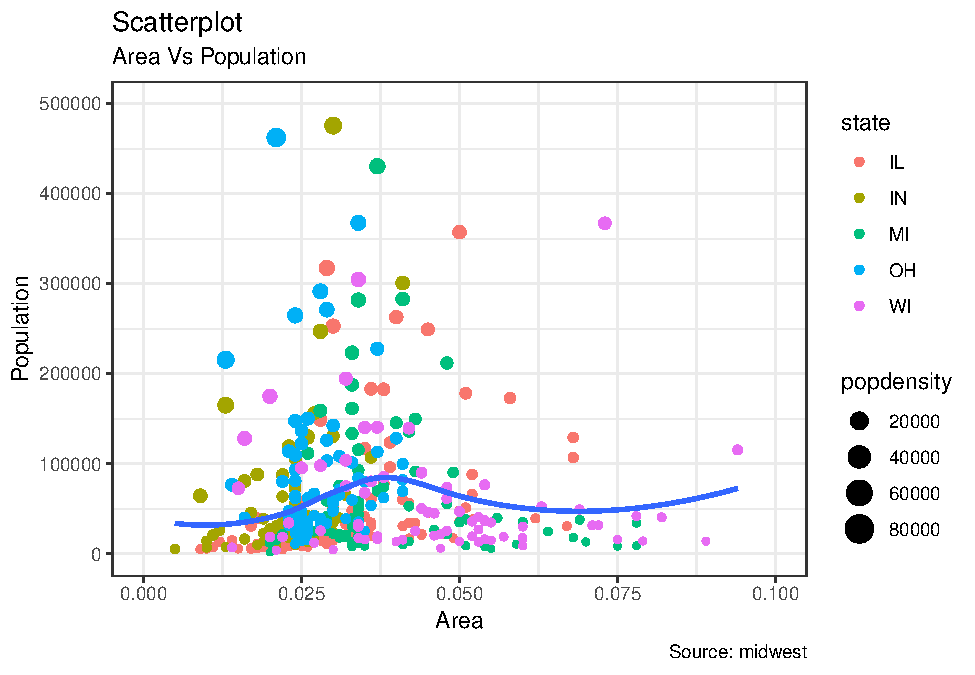
\includegraphics{ggplot2-50examples_files/figure-latex/unnamed-chunk-1-1.pdf}
\newpage

\textbf{Scatterplot With Encircling}

When presenting the results, sometimes I would encirlce certain special
group of points or region in the chart so as to draw the attention to
those peculiar cases. This can be conveniently done using the
\texttt{geom\_encircle()} in ggalt package.

Within \texttt{geom\_encircle()}, set the data to a new dataframe that
contains only the points (rows) or interest. Moreover, You can expand
the curve so as to pass just outside the points. The color and size
(thickness) of the curve can be modified as well. See below example.

\begin{Shaded}
\begin{Highlighting}[]
\CommentTok{# install 'ggalt' pkg}
\CommentTok{# devtools::install_github("hrbrmstr/ggalt")}
\KeywordTok{options}\NormalTok{(}\DataTypeTok{scipen =} \DecValTok{999}\NormalTok{)}
\KeywordTok{library}\NormalTok{(ggplot2)}
\KeywordTok{library}\NormalTok{(ggalt)}
\NormalTok{midwest_select <-}\StringTok{ }\NormalTok{midwest[midwest}\OperatorTok{$}\NormalTok{poptotal }\OperatorTok{>}\StringTok{ }\DecValTok{350000} \OperatorTok{&}\StringTok{ }
\StringTok{                            }\NormalTok{midwest}\OperatorTok{$}\NormalTok{poptotal }\OperatorTok{<=}\StringTok{ }\DecValTok{500000} \OperatorTok{&}\StringTok{ }
\StringTok{                            }\NormalTok{midwest}\OperatorTok{$}\NormalTok{area }\OperatorTok{>}\StringTok{ }\FloatTok{0.01} \OperatorTok{&}\StringTok{ }
\StringTok{                            }\NormalTok{midwest}\OperatorTok{$}\NormalTok{area }\OperatorTok{<}\StringTok{ }\FloatTok{0.1}\NormalTok{, ]}

\CommentTok{# Plot}
\KeywordTok{ggplot}\NormalTok{(midwest, }\KeywordTok{aes}\NormalTok{(}\DataTypeTok{x=}\NormalTok{area, }\DataTypeTok{y=}\NormalTok{poptotal)) }\OperatorTok{+}\StringTok{ }
\StringTok{  }\KeywordTok{geom_point}\NormalTok{(}\KeywordTok{aes}\NormalTok{(}\DataTypeTok{col=}\NormalTok{state, }\DataTypeTok{size=}\NormalTok{popdensity)) }\OperatorTok{+}\StringTok{   }\CommentTok{# draw points}
\StringTok{  }\KeywordTok{geom_smooth}\NormalTok{(}\DataTypeTok{method=}\StringTok{"loess"}\NormalTok{, }\DataTypeTok{se=}\NormalTok{F) }\OperatorTok{+}\StringTok{ }
\StringTok{  }\KeywordTok{xlim}\NormalTok{(}\KeywordTok{c}\NormalTok{(}\DecValTok{0}\NormalTok{, }\FloatTok{0.1}\NormalTok{)) }\OperatorTok{+}\StringTok{ }
\StringTok{  }\KeywordTok{ylim}\NormalTok{(}\KeywordTok{c}\NormalTok{(}\DecValTok{0}\NormalTok{, }\DecValTok{500000}\NormalTok{)) }\OperatorTok{+}\StringTok{   }\CommentTok{# draw smoothing line}
\StringTok{  }\KeywordTok{geom_encircle}\NormalTok{(}\KeywordTok{aes}\NormalTok{(}\DataTypeTok{x=}\NormalTok{area, }\DataTypeTok{y=}\NormalTok{poptotal), }
                \DataTypeTok{data=}\NormalTok{midwest_select, }
                \DataTypeTok{color=}\StringTok{"red"}\NormalTok{, }
                \DataTypeTok{size=}\DecValTok{2}\NormalTok{, }
                \DataTypeTok{expand=}\FloatTok{0.08}\NormalTok{) }\OperatorTok{+}\StringTok{   }\CommentTok{# encircle}
\StringTok{  }\KeywordTok{labs}\NormalTok{(}\DataTypeTok{subtitle=}\StringTok{"Area Vs Population"}\NormalTok{, }
       \DataTypeTok{y=}\StringTok{"Population"}\NormalTok{, }
       \DataTypeTok{x=}\StringTok{"Area"}\NormalTok{, }
       \DataTypeTok{title=}\StringTok{"Scatterplot + Encircle"}\NormalTok{, }
       \DataTypeTok{caption=}\StringTok{"Source: midwest"}\NormalTok{)}
\end{Highlighting}
\end{Shaded}

\begin{verbatim}
## Warning: Removed 15 rows containing non-finite values (stat_smooth).
\end{verbatim}

\begin{verbatim}
## Warning: Removed 15 rows containing missing values (geom_point).
\end{verbatim}

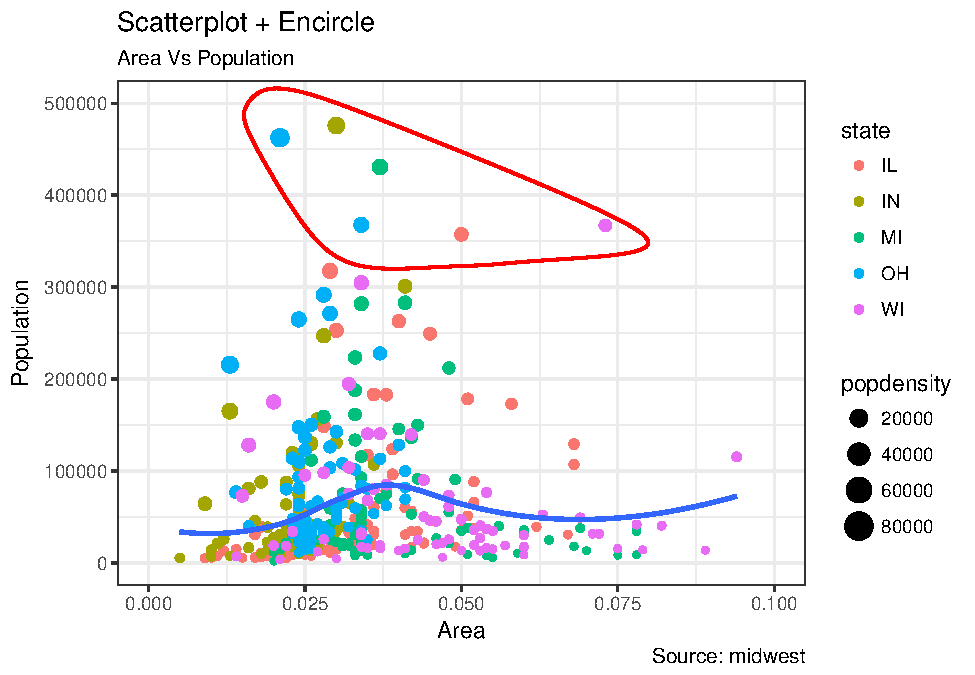
\includegraphics{ggplot2-50examples_files/figure-latex/unnamed-chunk-2-1.pdf}
\newpage

\textbf{Jitter Plot}

Let's look at a new data to draw the scatterplot. This time, I will use
the mpg dataset to plot city mileage (cty) vs highway mileage (hwy).

\begin{Shaded}
\begin{Highlighting}[]
\CommentTok{# load package and data}
\KeywordTok{library}\NormalTok{(ggplot2)}
\KeywordTok{data}\NormalTok{(mpg, }\DataTypeTok{package=}\StringTok{"ggplot2"}\NormalTok{) }\CommentTok{# alternate source: "http://goo.gl/uEeRGu")}
\KeywordTok{theme_set}\NormalTok{(}\KeywordTok{theme_bw}\NormalTok{())  }\CommentTok{# pre-set the bw theme.}

\NormalTok{g <-}\StringTok{ }\KeywordTok{ggplot}\NormalTok{(mpg, }\KeywordTok{aes}\NormalTok{(cty, hwy))}

\CommentTok{# Scatterplot}
\NormalTok{g }\OperatorTok{+}\StringTok{ }\KeywordTok{geom_point}\NormalTok{() }\OperatorTok{+}\StringTok{ }
\StringTok{  }\KeywordTok{geom_smooth}\NormalTok{(}\DataTypeTok{method=}\StringTok{"lm"}\NormalTok{, }\DataTypeTok{se=}\NormalTok{F) }\OperatorTok{+}
\StringTok{  }\KeywordTok{labs}\NormalTok{(}\DataTypeTok{subtitle=}\StringTok{"mpg: city vs highway mileage"}\NormalTok{, }
       \DataTypeTok{y=}\StringTok{"hwy"}\NormalTok{, }
       \DataTypeTok{x=}\StringTok{"cty"}\NormalTok{, }
       \DataTypeTok{title=}\StringTok{"Scatterplot with overlapping points"}\NormalTok{, }
       \DataTypeTok{caption=}\StringTok{"Source: midwest"}\NormalTok{)}
\end{Highlighting}
\end{Shaded}

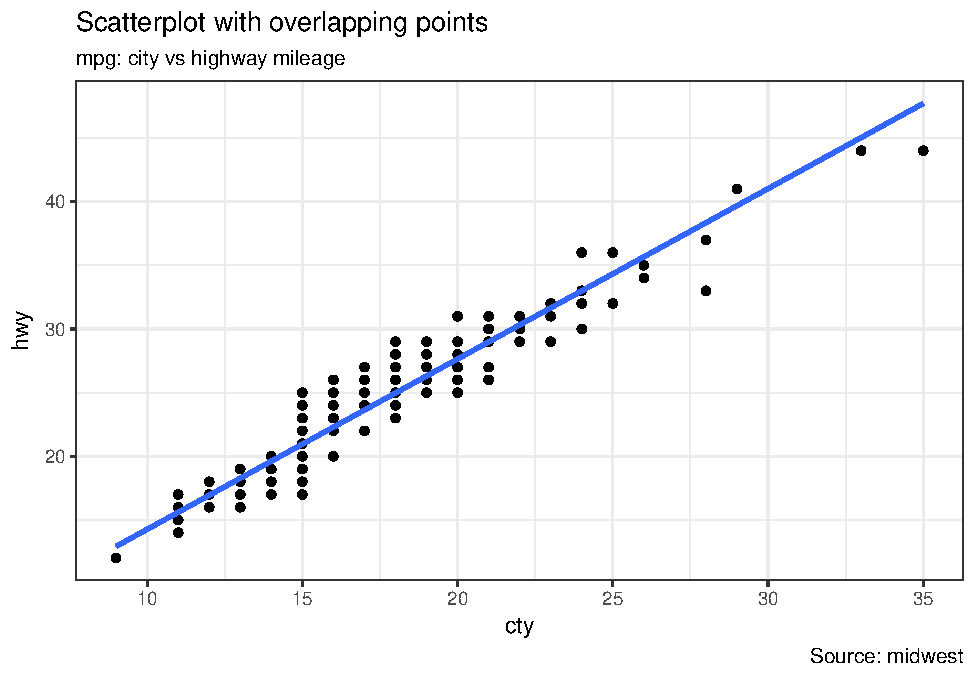
\includegraphics{ggplot2-50examples_files/figure-latex/unnamed-chunk-3-1.pdf}
\newpage

What we have here is a scatterplot of city and highway mileage in mpg
dataset. We have seen a similar scatterplot and this looks neat and
gives a clear idea of how the city mileage (cty) and highway mileage
(hwy) are well correlated.

But, this innocent looking plot is hiding something. Can you find out?

\begin{Shaded}
\begin{Highlighting}[]
\KeywordTok{dim}\NormalTok{(mpg)}
\end{Highlighting}
\end{Shaded}

\begin{verbatim}
## [1] 234  11
\end{verbatim}

The original data has 234 data points but the chart seems to display
fewer points. What has happened? This is because there are many
overlapping points appearing as a single dot. The fact that both cty and
hwy are integers in the source dataset made it all the more convenient
to hide this detail. So just be extra careful the next time you make
scatterplot with integers.

So how to handle this? There are few options. We can make a jitter plot
with \texttt{jitter\_geom()}. As the name suggests, the overlapping
points are randomly jittered around its original position based on a
threshold controlled by the \texttt{width} argument.

\begin{Shaded}
\begin{Highlighting}[]
\CommentTok{# load package and data}
\KeywordTok{library}\NormalTok{(ggplot2)}
\KeywordTok{data}\NormalTok{(mpg, }\DataTypeTok{package=}\StringTok{"ggplot2"}\NormalTok{)}
\CommentTok{# mpg <- read.csv("http://goo.gl/uEeRGu")}

\CommentTok{# Scatterplot}
\KeywordTok{theme_set}\NormalTok{(}\KeywordTok{theme_bw}\NormalTok{())  }\CommentTok{# pre-set the bw theme.}
\NormalTok{g <-}\StringTok{ }\KeywordTok{ggplot}\NormalTok{(mpg, }\KeywordTok{aes}\NormalTok{(cty, hwy))}
\NormalTok{g }\OperatorTok{+}\StringTok{ }\KeywordTok{geom_jitter}\NormalTok{(}\DataTypeTok{width =}\NormalTok{ .}\DecValTok{5}\NormalTok{, }\DataTypeTok{size=}\DecValTok{1}\NormalTok{) }\OperatorTok{+}
\StringTok{  }\KeywordTok{labs}\NormalTok{(}\DataTypeTok{subtitle=}\StringTok{"mpg: city vs highway mileage"}\NormalTok{, }
       \DataTypeTok{y=}\StringTok{"hwy"}\NormalTok{, }
       \DataTypeTok{x=}\StringTok{"cty"}\NormalTok{, }
       \DataTypeTok{title=}\StringTok{"Jittered Points"}\NormalTok{)}
\end{Highlighting}
\end{Shaded}

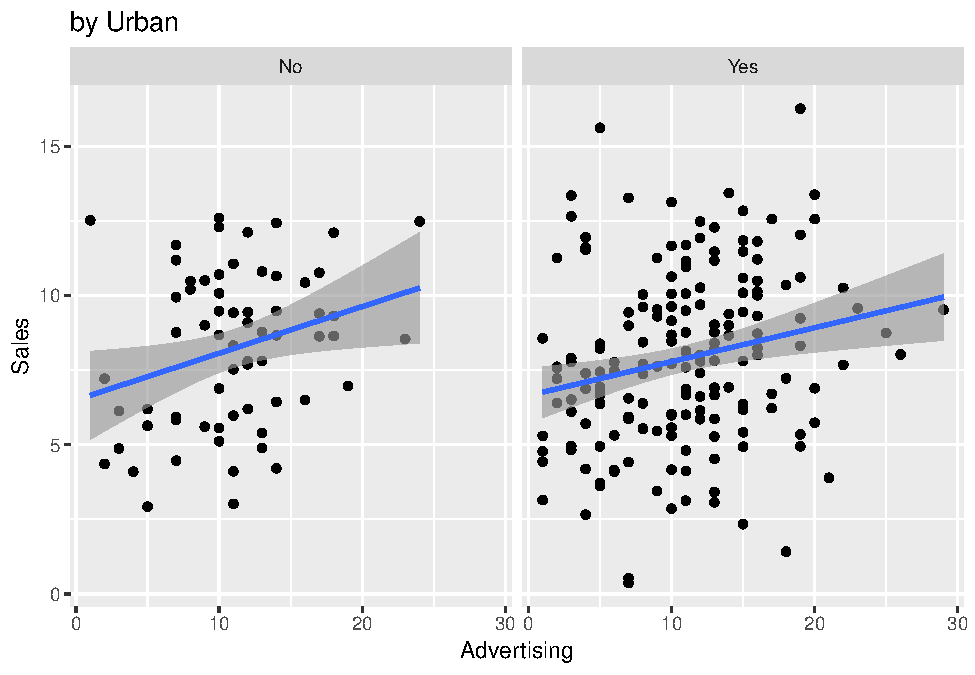
\includegraphics{ggplot2-50examples_files/figure-latex/unnamed-chunk-5-1.pdf}

More points are revealed now. More the width, more the points are moved
jittered from their original position.

\newpage

\textbf{Counts Chart}

The second option to overcome the problem of data points overlap is to
use what is called a counts chart. Whereever there is more points
overlap, the size of the circle gets bigger.

\begin{Shaded}
\begin{Highlighting}[]
\CommentTok{# load package and data}
\KeywordTok{library}\NormalTok{(ggplot2)}
\KeywordTok{data}\NormalTok{(mpg, }\DataTypeTok{package=}\StringTok{"ggplot2"}\NormalTok{)}
\CommentTok{# mpg <- read.csv("http://goo.gl/uEeRGu")}

\CommentTok{# Scatterplot}
\KeywordTok{theme_set}\NormalTok{(}\KeywordTok{theme_bw}\NormalTok{())  }\CommentTok{# pre-set the bw theme.}
\NormalTok{g <-}\StringTok{ }\KeywordTok{ggplot}\NormalTok{(mpg, }\KeywordTok{aes}\NormalTok{(cty, hwy))}
\NormalTok{g }\OperatorTok{+}\StringTok{ }\KeywordTok{geom_count}\NormalTok{(}\DataTypeTok{col=}\StringTok{"tomato3"}\NormalTok{, }\DataTypeTok{show.legend=}\NormalTok{F) }\OperatorTok{+}
\StringTok{  }\KeywordTok{labs}\NormalTok{(}\DataTypeTok{subtitle=}\StringTok{"mpg: city vs highway mileage"}\NormalTok{, }
       \DataTypeTok{y=}\StringTok{"hwy"}\NormalTok{, }
       \DataTypeTok{x=}\StringTok{"cty"}\NormalTok{, }
       \DataTypeTok{title=}\StringTok{"Counts Plot"}\NormalTok{)}
\end{Highlighting}
\end{Shaded}

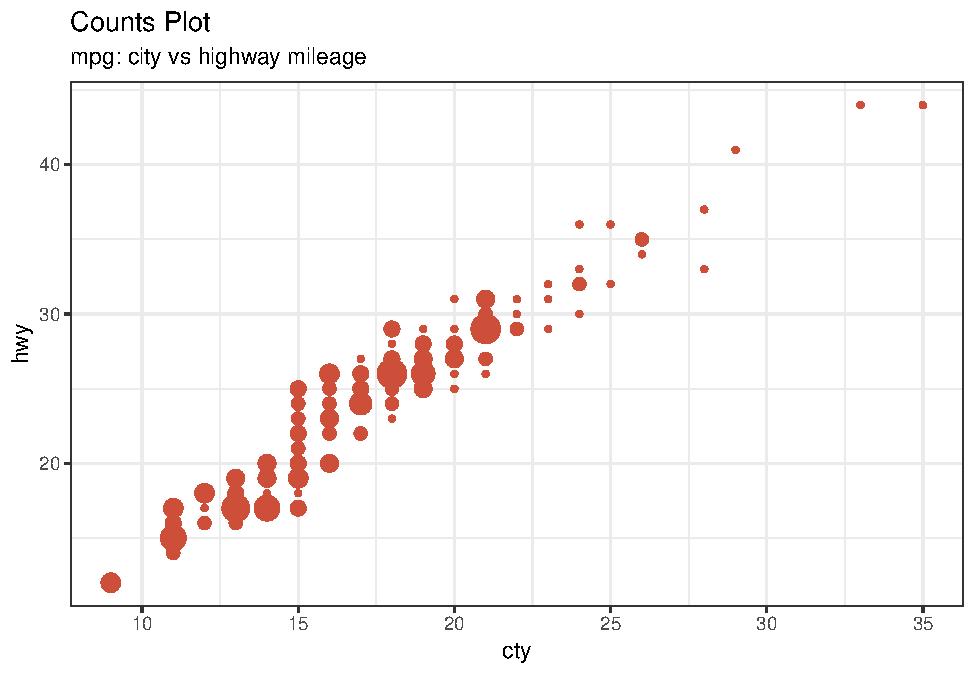
\includegraphics{ggplot2-50examples_files/figure-latex/unnamed-chunk-6-1.pdf}
\newpage

\textbf{Bubble plot}

While scatterplot lets you compare the relationship between 2 continuous
variables, bubble chart serves well if you want to understand
relationship within the underlying groups based on:

\begin{quote}
A Categorical variable (by changing the color) and Another continuous
variable (by changing the size of points).
\end{quote}

In simpler words, bubble charts are more suitable if you have
4-Dimensional data where two of them are numeric (X and Y) and one other
categorical (color) and another numeric variable (size).

The bubble chart clearly distinguishes the range of displ between the
manufacturers and how the slope of lines-of-best-fit varies, providing a
better visual comparison between the groups.

\begin{Shaded}
\begin{Highlighting}[]
\CommentTok{# load package and data}
\KeywordTok{library}\NormalTok{(ggplot2)}
\KeywordTok{data}\NormalTok{(mpg, }\DataTypeTok{package=}\StringTok{"ggplot2"}\NormalTok{)}
\CommentTok{# mpg <- read.csv("http://goo.gl/uEeRGu")}

\NormalTok{mpg_select <-}\StringTok{ }\NormalTok{mpg[mpg}\OperatorTok{$}\NormalTok{manufacturer }\OperatorTok\StringTok{ }\KeywordTok{c}\NormalTok{(}\StringTok{"audi"}\NormalTok{, }\StringTok{"ford"}\NormalTok{, }\StringTok{"honda"}\NormalTok{, }\StringTok{"hyundai"}\NormalTok{), ]}

\CommentTok{# Scatterplot}
\KeywordTok{theme_set}\NormalTok{(}\KeywordTok{theme_bw}\NormalTok{())  }\CommentTok{# pre-set the bw theme.}
\NormalTok{g <-}\StringTok{ }\KeywordTok{ggplot}\NormalTok{(mpg_select, }\KeywordTok{aes}\NormalTok{(displ, cty)) }\OperatorTok{+}\StringTok{ }
\StringTok{  }\KeywordTok{labs}\NormalTok{(}\DataTypeTok{subtitle=}\StringTok{"mpg: Displacement vs City Mileage"}\NormalTok{,}
       \DataTypeTok{title=}\StringTok{"Bubble chart"}\NormalTok{)}

\NormalTok{g }\OperatorTok{+}\StringTok{ }\KeywordTok{geom_jitter}\NormalTok{(}\KeywordTok{aes}\NormalTok{(}\DataTypeTok{col=}\NormalTok{manufacturer, }\DataTypeTok{size=}\NormalTok{hwy)) }\OperatorTok{+}\StringTok{ }
\StringTok{  }\KeywordTok{geom_smooth}\NormalTok{(}\KeywordTok{aes}\NormalTok{(}\DataTypeTok{col=}\NormalTok{manufacturer), }\DataTypeTok{method=}\StringTok{"lm"}\NormalTok{, }\DataTypeTok{se=}\NormalTok{F)}
\end{Highlighting}
\end{Shaded}

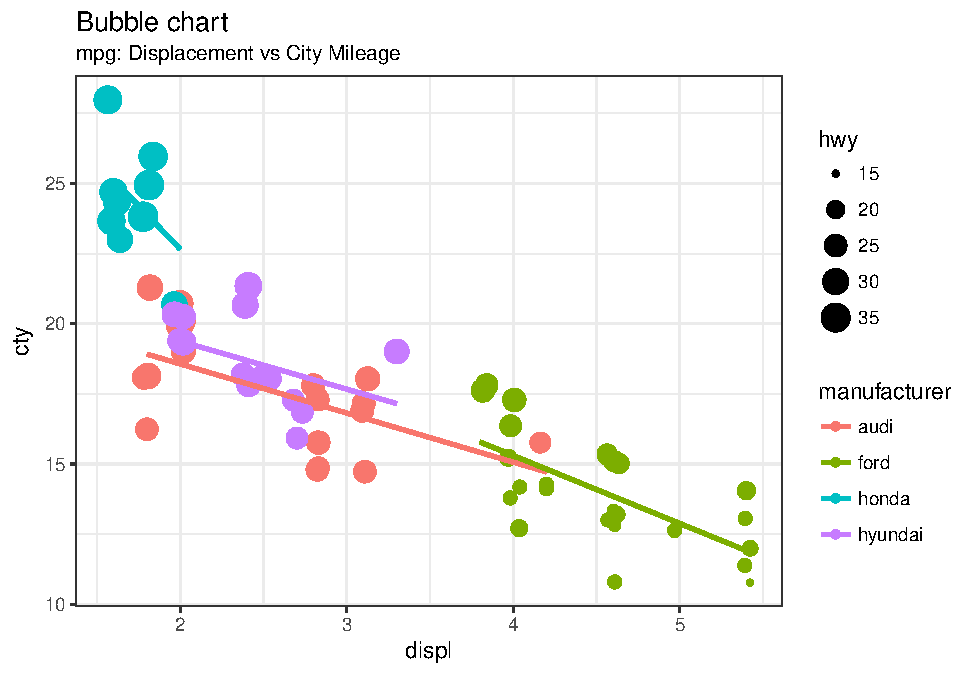
\includegraphics{ggplot2-50examples_files/figure-latex/unnamed-chunk-7-1.pdf}
\newpage

\newpage

\textbf{Marginal Histogram / Boxplot}

If you want to show the relationship as well as the distribution in the
same chart, use the marginal histogram. It has a histogram of the X and
Y variables at the margins of the scatterplot.

This can be implemented using the ggMarginal() function from the
`ggExtra' package. Apart from a histogram, you could choose to draw a
marginal boxplot or density plot by setting the respective type option.

\begin{Shaded}
\begin{Highlighting}[]
\CommentTok{# load package and data}
\KeywordTok{library}\NormalTok{(ggplot2)}
\KeywordTok{library}\NormalTok{(ggExtra)}
\KeywordTok{data}\NormalTok{(mpg, }\DataTypeTok{package=}\StringTok{"ggplot2"}\NormalTok{)}
\CommentTok{# mpg <- read.csv("http://goo.gl/uEeRGu")}

\CommentTok{# Scatterplot}
\KeywordTok{theme_set}\NormalTok{(}\KeywordTok{theme_bw}\NormalTok{())  }\CommentTok{# pre-set the bw theme.}
\NormalTok{mpg_select <-}\StringTok{ }\NormalTok{mpg[mpg}\OperatorTok{$}\NormalTok{hwy }\OperatorTok{>=}\StringTok{ }\DecValTok{35} \OperatorTok{&}\StringTok{ }\NormalTok{mpg}\OperatorTok{$}\NormalTok{cty }\OperatorTok{>}\StringTok{ }\DecValTok{27}\NormalTok{, ]}
\NormalTok{g <-}\StringTok{ }\KeywordTok{ggplot}\NormalTok{(mpg, }\KeywordTok{aes}\NormalTok{(cty, hwy)) }\OperatorTok{+}\StringTok{ }
\StringTok{  }\KeywordTok{geom_count}\NormalTok{() }\OperatorTok{+}\StringTok{ }
\StringTok{  }\KeywordTok{geom_smooth}\NormalTok{(}\DataTypeTok{method=}\StringTok{"lm"}\NormalTok{, }\DataTypeTok{se=}\NormalTok{F)}

\KeywordTok{ggMarginal}\NormalTok{(g, }\DataTypeTok{type =} \StringTok{"histogram"}\NormalTok{, }\DataTypeTok{fill=}\StringTok{"transparent"}\NormalTok{)}
\KeywordTok{ggMarginal}\NormalTok{(g, }\DataTypeTok{type =} \StringTok{"boxplot"}\NormalTok{, }\DataTypeTok{fill=}\StringTok{"transparent"}\NormalTok{)}
\end{Highlighting}
\end{Shaded}

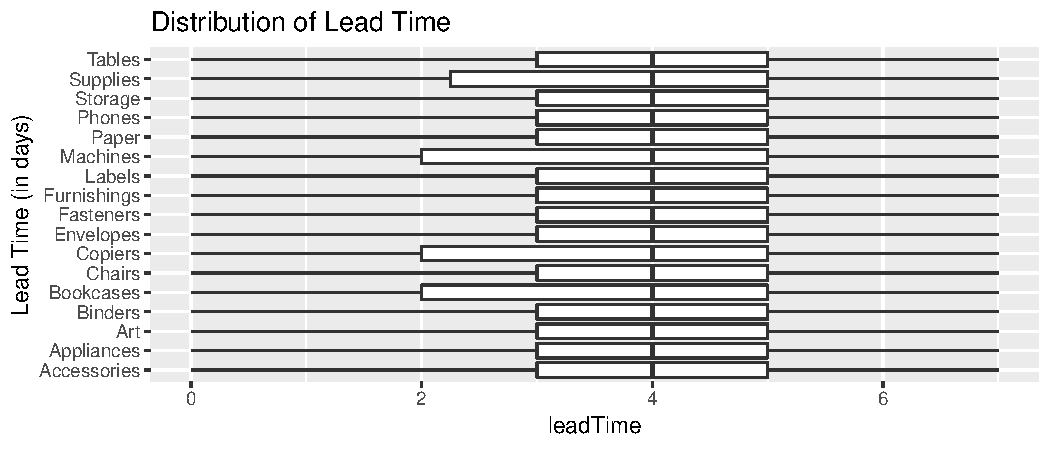
\includegraphics{ggplot2-50examples_files/figure-latex/unnamed-chunk-10-1.pdf}

\begin{Shaded}
\begin{Highlighting}[]
\CommentTok{# ggMarginal(g, type = "density", fill="transparent")}
\end{Highlighting}
\end{Shaded}

\newpage

\textbf{Correlogram}

Correlogram let's you examine the corellation of multiple continuous
variables present in the same dataframe. This is conveniently
implemented using the ggcorrplot package.

\begin{Shaded}
\begin{Highlighting}[]
\CommentTok{# devtools::install_github("kassambara/ggcorrplot")}
\KeywordTok{library}\NormalTok{(ggplot2)}
\KeywordTok{library}\NormalTok{(ggcorrplot)}

\CommentTok{# Correlation matrix}
\KeywordTok{data}\NormalTok{(mtcars)}
\NormalTok{corr <-}\StringTok{ }\KeywordTok{round}\NormalTok{(}\KeywordTok{cor}\NormalTok{(mtcars), }\DecValTok{1}\NormalTok{)}

\CommentTok{# Plot}
\KeywordTok{ggcorrplot}\NormalTok{(corr, }\DataTypeTok{hc.order =} \OtherTok{TRUE}\NormalTok{, }
           \DataTypeTok{type =} \StringTok{"lower"}\NormalTok{, }
           \DataTypeTok{lab =} \OtherTok{TRUE}\NormalTok{, }
           \DataTypeTok{lab_size =} \DecValTok{3}\NormalTok{, }
           \DataTypeTok{method=}\StringTok{"circle"}\NormalTok{, }
           \DataTypeTok{colors =} \KeywordTok{c}\NormalTok{(}\StringTok{"tomato2"}\NormalTok{, }\StringTok{"white"}\NormalTok{, }\StringTok{"springgreen3"}\NormalTok{), }
           \DataTypeTok{title=}\StringTok{"Correlogram of mtcars"}\NormalTok{, }
           \DataTypeTok{ggtheme=}\NormalTok{theme_bw)}
\end{Highlighting}
\end{Shaded}

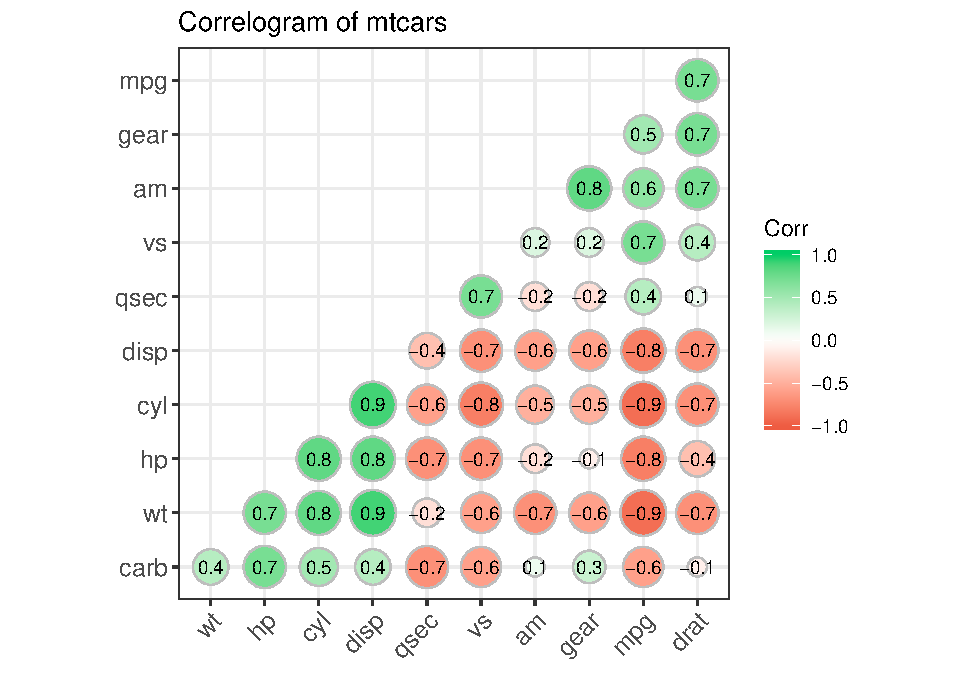
\includegraphics{ggplot2-50examples_files/figure-latex/unnamed-chunk-11-1.pdf}
\newpage

\subsection{2. Deviation}\label{deviation}

Compare variation in values between small number of items (or
categories) with respect to a fixed reference.

\textbf{Diverging bars}

Diverging Bars is a bar chart that can handle both negative and positive
values. This can be implemented by a smart tweak with
\texttt{geom\_bar()}. But the usage of \texttt{geom\_bar()} can be quite
confusing. Thats because, it can be used to make a bar chart as well as
a histogram. Let me explain.

By default, \texttt{geom\_bar()} has the stat set to count. That means,
when you provide just a continuous X variable (and no Y variable), it
tries to make a histogram out of the data.

In order to make a bar chart create bars instead of histogram, you need
to do two things.

\begin{quote}
Set \texttt{stat=identity} Provide both \texttt{x} and \texttt{y} inside
\texttt{aes()} where, \texttt{x} is either character or factor and
\texttt{y} is numeric. In order to make sure you get diverging bars
instead of just bars, make sure, your categorical variable has 2
categories that changes values at a certain threshold of the continuous
variable. In below example, the mpg from mtcars dataset is normalised by
computing the z score. Those vehicles with mpg above zero are marked
green and those below are marked red.
\end{quote}

\begin{Shaded}
\begin{Highlighting}[]
\KeywordTok{library}\NormalTok{(ggplot2)}
\KeywordTok{theme_set}\NormalTok{(}\KeywordTok{theme_bw}\NormalTok{())  }

\CommentTok{# Data Prep}
\KeywordTok{data}\NormalTok{(}\StringTok{"mtcars"}\NormalTok{)  }\CommentTok{# load data}
\NormalTok{mtcars}\OperatorTok{$}\StringTok{`}\DataTypeTok{car name}\StringTok{`}\NormalTok{ <-}\StringTok{ }\KeywordTok{rownames}\NormalTok{(mtcars)  }\CommentTok{# create new column for car names}
\NormalTok{mtcars}\OperatorTok{$}\NormalTok{mpg_z <-}\StringTok{ }\KeywordTok{round}\NormalTok{((mtcars}\OperatorTok{$}\NormalTok{mpg }\OperatorTok{-}\StringTok{ }\KeywordTok{mean}\NormalTok{(mtcars}\OperatorTok{$}\NormalTok{mpg))}\OperatorTok{/}\KeywordTok{sd}\NormalTok{(mtcars}\OperatorTok{$}\NormalTok{mpg), }\DecValTok{2}\NormalTok{)  }
\CommentTok{# compute normalized mpg}
\NormalTok{mtcars}\OperatorTok{$}\NormalTok{mpg_type <-}\StringTok{ }\KeywordTok{ifelse}\NormalTok{(mtcars}\OperatorTok{$}\NormalTok{mpg_z }\OperatorTok{<}\StringTok{ }\DecValTok{0}\NormalTok{, }\StringTok{"below"}\NormalTok{, }\StringTok{"above"}\NormalTok{)  }\CommentTok{# above / below avg flag}
\NormalTok{mtcars <-}\StringTok{ }\NormalTok{mtcars[}\KeywordTok{order}\NormalTok{(mtcars}\OperatorTok{$}\NormalTok{mpg_z), ]  }\CommentTok{# sort}
\NormalTok{mtcars}\OperatorTok{$}\StringTok{`}\DataTypeTok{car name}\StringTok{`}\NormalTok{ <-}\StringTok{ }\KeywordTok{factor}\NormalTok{(mtcars}\OperatorTok{$}\StringTok{`}\DataTypeTok{car name}\StringTok{`}\NormalTok{, }\DataTypeTok{levels =}\NormalTok{ mtcars}\OperatorTok{$}\StringTok{`}\DataTypeTok{car name}\StringTok{`}\NormalTok{)  }
\CommentTok{# convert to factor to retain sorted order in plot.}

\CommentTok{# Diverging Barcharts}
\KeywordTok{ggplot}\NormalTok{(mtcars, }\KeywordTok{aes}\NormalTok{(}\DataTypeTok{x=}\StringTok{`}\DataTypeTok{car name}\StringTok{`}\NormalTok{, }\DataTypeTok{y=}\NormalTok{mpg_z, }\DataTypeTok{label=}\NormalTok{mpg_z)) }\OperatorTok{+}\StringTok{ }
\StringTok{  }\KeywordTok{geom_bar}\NormalTok{(}\DataTypeTok{stat=}\StringTok{'identity'}\NormalTok{, }\KeywordTok{aes}\NormalTok{(}\DataTypeTok{fill=}\NormalTok{mpg_type), }\DataTypeTok{width=}\NormalTok{.}\DecValTok{5}\NormalTok{)  }\OperatorTok{+}
\StringTok{  }\KeywordTok{scale_fill_manual}\NormalTok{(}\DataTypeTok{name=}\StringTok{"Mileage"}\NormalTok{, }
                    \DataTypeTok{labels =} \KeywordTok{c}\NormalTok{(}\StringTok{"Above Average"}\NormalTok{, }\StringTok{"Below Average"}\NormalTok{), }
                    \DataTypeTok{values =} \KeywordTok{c}\NormalTok{(}\StringTok{"above"}\NormalTok{=}\StringTok{"#00ba38"}\NormalTok{, }\StringTok{"below"}\NormalTok{=}\StringTok{"#f8766d"}\NormalTok{)) }\OperatorTok{+}\StringTok{ }
\StringTok{  }\KeywordTok{labs}\NormalTok{(}\DataTypeTok{subtitle=}\StringTok{"Normalised mileage from 'mtcars'"}\NormalTok{, }
       \DataTypeTok{title=} \StringTok{"Diverging Bars"}\NormalTok{) }\OperatorTok{+}\StringTok{ }
\StringTok{  }\KeywordTok{coord_flip}\NormalTok{()}
\end{Highlighting}
\end{Shaded}

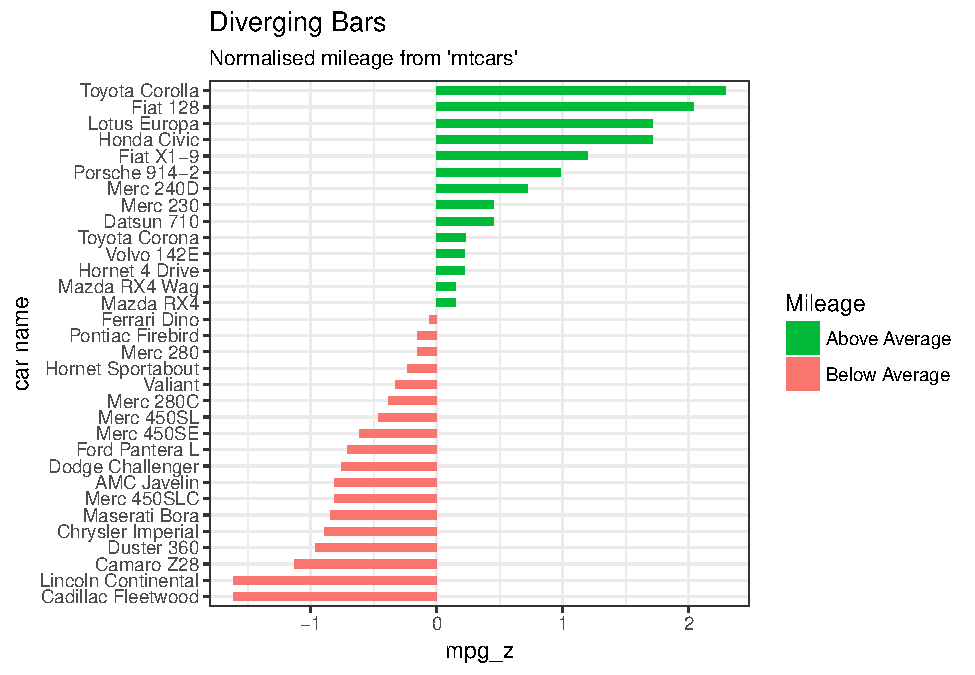
\includegraphics{ggplot2-50examples_files/figure-latex/unnamed-chunk-12-1.pdf}
\newpage

\textbf{Diverging Lollipop Chart}

Lollipop chart conveys the same information as bar chart and diverging
bar. Except that it looks more modern. Instead of geom\_bar, I use
geom\_point and geom\_segment to get the lollipops right. Let's draw a
lollipop using the same data I prepared in the previous example of
diverging bars.

\begin{Shaded}
\begin{Highlighting}[]
\KeywordTok{library}\NormalTok{(ggplot2)}
\KeywordTok{theme_set}\NormalTok{(}\KeywordTok{theme_bw}\NormalTok{())}

\KeywordTok{ggplot}\NormalTok{(mtcars, }\KeywordTok{aes}\NormalTok{(}\DataTypeTok{x=}\StringTok{`}\DataTypeTok{car name}\StringTok{`}\NormalTok{, }\DataTypeTok{y=}\NormalTok{mpg_z, }\DataTypeTok{label=}\NormalTok{mpg_z)) }\OperatorTok{+}\StringTok{ }
\StringTok{  }\KeywordTok{geom_point}\NormalTok{(}\DataTypeTok{stat=}\StringTok{'identity'}\NormalTok{, }\DataTypeTok{fill=}\StringTok{"black"}\NormalTok{, }\DataTypeTok{size=}\DecValTok{6}\NormalTok{)  }\OperatorTok{+}
\StringTok{  }\KeywordTok{geom_segment}\NormalTok{(}\KeywordTok{aes}\NormalTok{(}\DataTypeTok{y =} \DecValTok{0}\NormalTok{, }
                   \DataTypeTok{x =} \StringTok{`}\DataTypeTok{car name}\StringTok{`}\NormalTok{, }
                   \DataTypeTok{yend =}\NormalTok{ mpg_z, }
                   \DataTypeTok{xend =} \StringTok{`}\DataTypeTok{car name}\StringTok{`}\NormalTok{), }
               \DataTypeTok{color =} \StringTok{"black"}\NormalTok{) }\OperatorTok{+}
\StringTok{  }\KeywordTok{geom_text}\NormalTok{(}\DataTypeTok{color=}\StringTok{"white"}\NormalTok{, }\DataTypeTok{size=}\DecValTok{2}\NormalTok{) }\OperatorTok{+}
\StringTok{  }\KeywordTok{labs}\NormalTok{(}\DataTypeTok{title=}\StringTok{"Diverging Lollipop Chart"}\NormalTok{, }
       \DataTypeTok{subtitle=}\StringTok{"Normalized mileage from 'mtcars': Lollipop"}\NormalTok{) }\OperatorTok{+}\StringTok{ }
\StringTok{  }\KeywordTok{ylim}\NormalTok{(}\OperatorTok{-}\FloatTok{2.5}\NormalTok{, }\FloatTok{2.5}\NormalTok{) }\OperatorTok{+}
\StringTok{  }\KeywordTok{coord_flip}\NormalTok{()}
\end{Highlighting}
\end{Shaded}

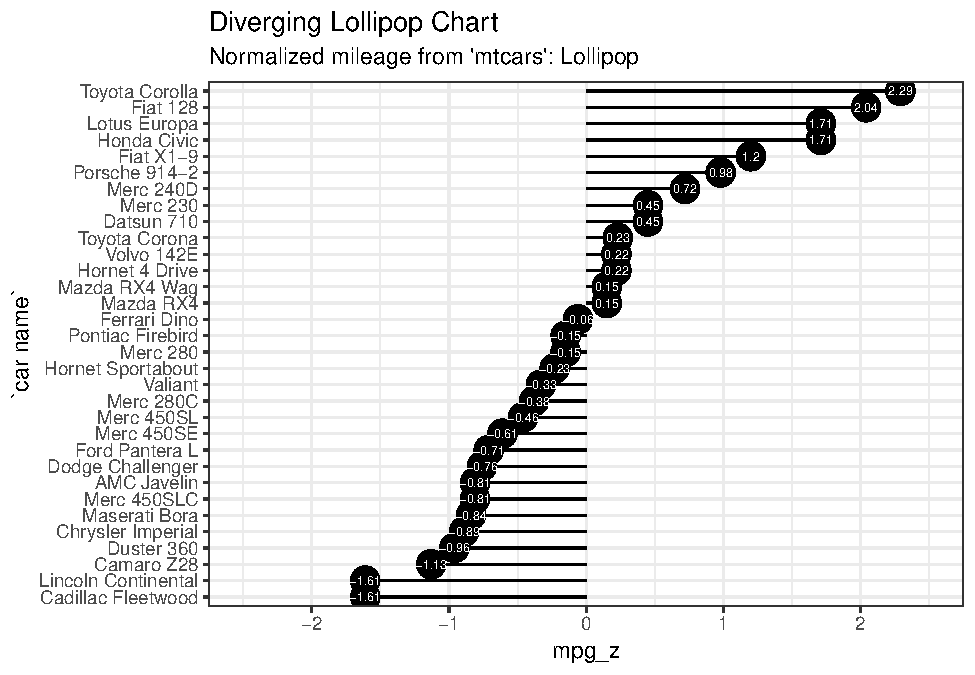
\includegraphics{ggplot2-50examples_files/figure-latex/unnamed-chunk-13-1.pdf}
\newpage

\textbf{Diverging Dot Plot}

Dot plot conveys similar information. The principles are same as what we
saw in Diverging bars, except that only point are used. Below example
uses the same data prepared in the diverging bars example.

\begin{Shaded}
\begin{Highlighting}[]
\KeywordTok{library}\NormalTok{(ggplot2)}
\KeywordTok{theme_set}\NormalTok{(}\KeywordTok{theme_bw}\NormalTok{())}

\CommentTok{# Plot}
\KeywordTok{ggplot}\NormalTok{(mtcars, }\KeywordTok{aes}\NormalTok{(}\DataTypeTok{x=}\StringTok{`}\DataTypeTok{car name}\StringTok{`}\NormalTok{, }\DataTypeTok{y=}\NormalTok{mpg_z, }\DataTypeTok{label=}\NormalTok{mpg_z)) }\OperatorTok{+}\StringTok{ }
\StringTok{  }\KeywordTok{geom_point}\NormalTok{(}\DataTypeTok{stat=}\StringTok{'identity'}\NormalTok{, }\KeywordTok{aes}\NormalTok{(}\DataTypeTok{col=}\NormalTok{mpg_type), }\DataTypeTok{size=}\DecValTok{6}\NormalTok{)  }\OperatorTok{+}
\StringTok{  }\KeywordTok{scale_color_manual}\NormalTok{(}\DataTypeTok{name=}\StringTok{"Mileage"}\NormalTok{, }
                     \DataTypeTok{labels =} \KeywordTok{c}\NormalTok{(}\StringTok{"Above Average"}\NormalTok{, }\StringTok{"Below Average"}\NormalTok{), }
                     \DataTypeTok{values =} \KeywordTok{c}\NormalTok{(}\StringTok{"above"}\NormalTok{=}\StringTok{"#00ba38"}\NormalTok{, }\StringTok{"below"}\NormalTok{=}\StringTok{"#f8766d"}\NormalTok{)) }\OperatorTok{+}\StringTok{ }
\StringTok{  }\KeywordTok{geom_text}\NormalTok{(}\DataTypeTok{color=}\StringTok{"white"}\NormalTok{, }\DataTypeTok{size=}\DecValTok{2}\NormalTok{) }\OperatorTok{+}
\StringTok{  }\KeywordTok{labs}\NormalTok{(}\DataTypeTok{title=}\StringTok{"Diverging Dot Plot"}\NormalTok{, }
       \DataTypeTok{subtitle=}\StringTok{"Normalized mileage from 'mtcars': Dotplot"}\NormalTok{) }\OperatorTok{+}\StringTok{ }
\StringTok{  }\KeywordTok{ylim}\NormalTok{(}\OperatorTok{-}\FloatTok{2.5}\NormalTok{, }\FloatTok{2.5}\NormalTok{) }\OperatorTok{+}
\StringTok{  }\KeywordTok{coord_flip}\NormalTok{()}
\end{Highlighting}
\end{Shaded}

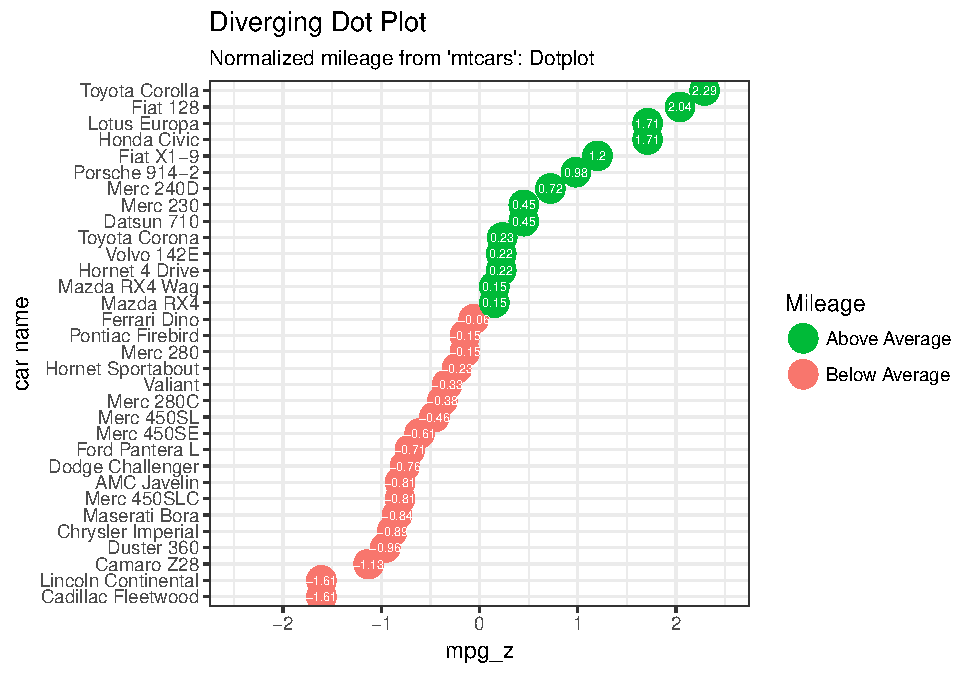
\includegraphics{ggplot2-50examples_files/figure-latex/unnamed-chunk-14-1.pdf}
\newpage

\textbf{Area Chart}

Area charts are typically used to visualize how a particular metric
(such as \% returns from a stock) performed compared to a certain
baseline. Other types of \%returns or \%change data are also commonly
used. The \texttt{geom\_area()} implements this.

\begin{Shaded}
\begin{Highlighting}[]
\KeywordTok{library}\NormalTok{(ggplot2)}
\KeywordTok{library}\NormalTok{(quantmod)}
\end{Highlighting}
\end{Shaded}

\begin{verbatim}
## Loading required package: xts
\end{verbatim}

\begin{verbatim}
## Loading required package: zoo
\end{verbatim}

\begin{verbatim}
## 
## Attaching package: 'zoo'
\end{verbatim}

\begin{verbatim}
## The following objects are masked from 'package:base':
## 
##     as.Date, as.Date.numeric
\end{verbatim}

\begin{verbatim}
## Loading required package: TTR
\end{verbatim}

\begin{verbatim}
## Version 0.4-0 included new data defaults. See ?getSymbols.
\end{verbatim}

\begin{Shaded}
\begin{Highlighting}[]
\KeywordTok{data}\NormalTok{(}\StringTok{"economics"}\NormalTok{, }\DataTypeTok{package =} \StringTok{"ggplot2"}\NormalTok{)}

\CommentTok{# Compute % Returns}
\NormalTok{economics}\OperatorTok{$}\NormalTok{returns_perc <-}\StringTok{ }
\StringTok{  }\KeywordTok{c}\NormalTok{(}\DecValTok{0}\NormalTok{, }\KeywordTok{diff}\NormalTok{(economics}\OperatorTok{$}\NormalTok{psavert)}\OperatorTok{/}\NormalTok{economics}\OperatorTok{$}\NormalTok{psavert[}\OperatorTok{-}\KeywordTok{length}\NormalTok{(economics}\OperatorTok{$}\NormalTok{psavert)])}

\CommentTok{# Create break points and labels for axis ticks}
\NormalTok{brks <-}\StringTok{ }\NormalTok{economics}\OperatorTok{$}\NormalTok{date[}\KeywordTok{seq}\NormalTok{(}\DecValTok{1}\NormalTok{, }\KeywordTok{length}\NormalTok{(economics}\OperatorTok{$}\NormalTok{date), }\DecValTok{12}\NormalTok{)]}
\NormalTok{lbls <-}\StringTok{ }\NormalTok{lubridate}\OperatorTok{::}\KeywordTok{year}\NormalTok{(economics}\OperatorTok{$}\NormalTok{date[}\KeywordTok{seq}\NormalTok{(}\DecValTok{1}\NormalTok{, }\KeywordTok{length}\NormalTok{(economics}\OperatorTok{$}\NormalTok{date), }\DecValTok{12}\NormalTok{)])}

\CommentTok{# Plot}
\KeywordTok{ggplot}\NormalTok{(economics[}\DecValTok{1}\OperatorTok{:}\DecValTok{100}\NormalTok{, ], }\KeywordTok{aes}\NormalTok{(date, returns_perc)) }\OperatorTok{+}\StringTok{ }
\StringTok{  }\KeywordTok{geom_area}\NormalTok{() }\OperatorTok{+}\StringTok{ }
\StringTok{  }\KeywordTok{scale_x_date}\NormalTok{(}\DataTypeTok{breaks=}\NormalTok{brks, }\DataTypeTok{labels=}\NormalTok{lbls) }\OperatorTok{+}\StringTok{ }
\StringTok{  }\KeywordTok{theme}\NormalTok{(}\DataTypeTok{axis.text.x =} \KeywordTok{element_text}\NormalTok{(}\DataTypeTok{angle=}\DecValTok{90}\NormalTok{)) }\OperatorTok{+}\StringTok{ }
\StringTok{  }\KeywordTok{labs}\NormalTok{(}\DataTypeTok{title=}\StringTok{"Area Chart"}\NormalTok{, }
       \DataTypeTok{subtitle =} \StringTok{"Perc Returns for Personal Savings"}\NormalTok{, }
       \DataTypeTok{y=}\StringTok{"% Returns for Personal savings"}\NormalTok{, }
       \DataTypeTok{caption=}\StringTok{"Source: economics"}\NormalTok{)}
\end{Highlighting}
\end{Shaded}

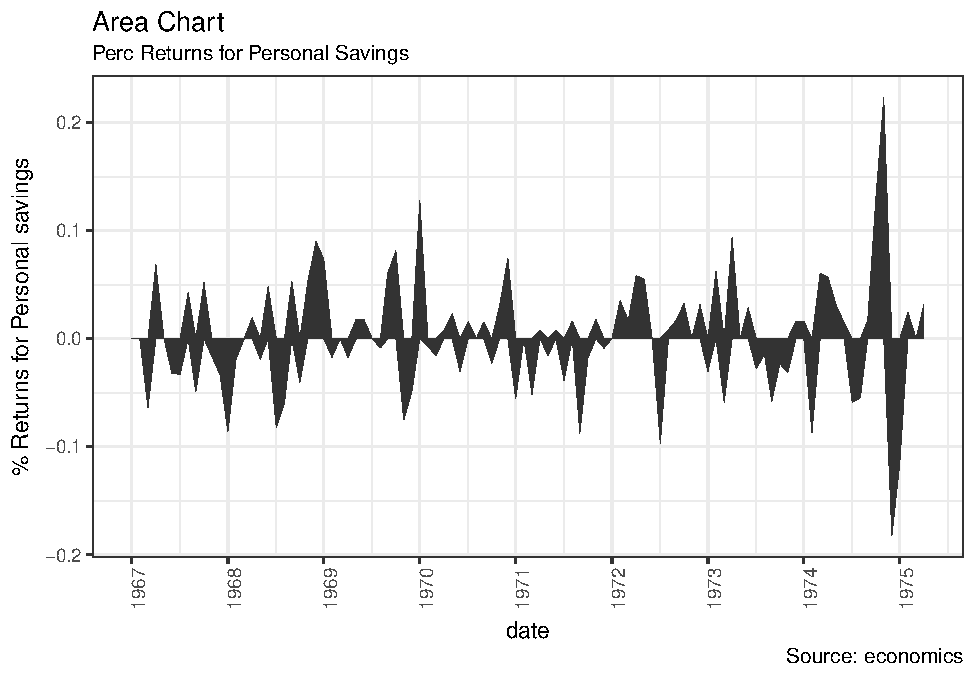
\includegraphics{ggplot2-50examples_files/figure-latex/unnamed-chunk-15-1.pdf}

\newpage

\subsection{3. Ranking}\label{ranking}

Used to compare the position or performance of multiple items with
respect to each other. Actual values matters somewhat less than the
ranking.

\textbf{Ordered Bar Chart}

Ordered Bar Chart is a Bar Chart that is ordered by the Y axis variable.
Just sorting the dataframe by the variable of interest isn't enough to
order the bar chart. In order for the bar chart to retain the order of
the rows, the X axis variable (i.e.~the categories) has to be converted
into a factor.

Let's plot the mean city mileage for each manufacturer from mpg dataset.
First, aggregate the data and sort it before you draw the plot. Finally,
the X variable is converted to a factor.

Let's see how that is done.

\begin{Shaded}
\begin{Highlighting}[]
\CommentTok{# Prepare data - group mean city mileage by manufacturer.  }
\NormalTok{cty_mpg <-}\StringTok{ }\KeywordTok{aggregate}\NormalTok{(mpg}\OperatorTok{$}\NormalTok{cty, }\DataTypeTok{by=}\KeywordTok{list}\NormalTok{(mpg}\OperatorTok{$}\NormalTok{manufacturer), }\DataTypeTok{FUN=}\NormalTok{mean)  }\CommentTok{# aggregate}
\KeywordTok{colnames}\NormalTok{(cty_mpg) <-}\StringTok{ }\KeywordTok{c}\NormalTok{(}\StringTok{"make"}\NormalTok{, }\StringTok{"mileage"}\NormalTok{)  }\CommentTok{# change column names}
\NormalTok{cty_mpg <-}\StringTok{ }\NormalTok{cty_mpg[}\KeywordTok{order}\NormalTok{(cty_mpg}\OperatorTok{$}\NormalTok{mileage), ]  }\CommentTok{# sort}
\NormalTok{cty_mpg}\OperatorTok{$}\NormalTok{make <-}\StringTok{ }\KeywordTok{factor}\NormalTok{(cty_mpg}\OperatorTok{$}\NormalTok{make, }\DataTypeTok{levels =}\NormalTok{ cty_mpg}\OperatorTok{$}\NormalTok{make)  }
\CommentTok{# to retain the order in plot.}
\KeywordTok{head}\NormalTok{(cty_mpg, }\DecValTok{4}\NormalTok{)}
\end{Highlighting}
\end{Shaded}

\begin{verbatim}
##          make  mileage
## 9     lincoln 11.33333
## 8  land rover 11.50000
## 3       dodge 13.13514
## 10    mercury 13.25000
\end{verbatim}

The X variable is now a factor, let's plot.

\begin{Shaded}
\begin{Highlighting}[]
\KeywordTok{library}\NormalTok{(ggplot2)}
\KeywordTok{theme_set}\NormalTok{(}\KeywordTok{theme_bw}\NormalTok{())}

\CommentTok{# Draw plot}
\KeywordTok{ggplot}\NormalTok{(cty_mpg, }\KeywordTok{aes}\NormalTok{(}\DataTypeTok{x=}\NormalTok{make, }\DataTypeTok{y=}\NormalTok{mileage)) }\OperatorTok{+}\StringTok{ }
\StringTok{  }\KeywordTok{geom_bar}\NormalTok{(}\DataTypeTok{stat=}\StringTok{"identity"}\NormalTok{, }\DataTypeTok{width=}\NormalTok{.}\DecValTok{5}\NormalTok{, }\DataTypeTok{fill=}\StringTok{"tomato3"}\NormalTok{) }\OperatorTok{+}\StringTok{ }
\StringTok{  }\KeywordTok{labs}\NormalTok{(}\DataTypeTok{title=}\StringTok{"Ordered Bar Chart"}\NormalTok{, }
       \DataTypeTok{subtitle=}\StringTok{"Make Vs Avg. Mileage"}\NormalTok{, }
       \DataTypeTok{caption=}\StringTok{"source: mpg"}\NormalTok{) }\OperatorTok{+}\StringTok{ }
\StringTok{  }\KeywordTok{theme}\NormalTok{(}\DataTypeTok{axis.text.x =} \KeywordTok{element_text}\NormalTok{(}\DataTypeTok{angle=}\DecValTok{65}\NormalTok{, }\DataTypeTok{vjust=}\FloatTok{0.6}\NormalTok{))}
\end{Highlighting}
\end{Shaded}

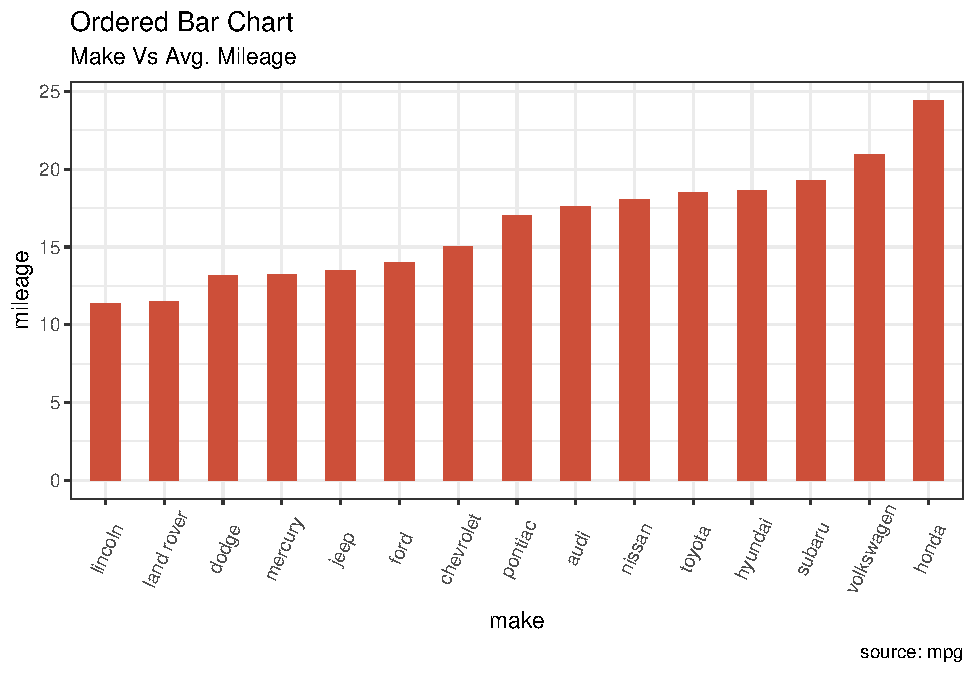
\includegraphics{ggplot2-50examples_files/figure-latex/unnamed-chunk-17-1.pdf}

\newpage

\textbf{Lollipop Chart}

Lollipop charts conveys the same information as in bar charts. By
reducing the thick bars into thin lines, it reduces the clutter and lays
more emphasis on the value. It looks nice and modern.

\begin{Shaded}
\begin{Highlighting}[]
\KeywordTok{library}\NormalTok{(ggplot2)}
\KeywordTok{theme_set}\NormalTok{(}\KeywordTok{theme_bw}\NormalTok{())}

\CommentTok{# Plot}
\KeywordTok{ggplot}\NormalTok{(cty_mpg, }\KeywordTok{aes}\NormalTok{(}\DataTypeTok{x=}\NormalTok{make, }\DataTypeTok{y=}\NormalTok{mileage)) }\OperatorTok{+}\StringTok{ }
\StringTok{  }\KeywordTok{geom_point}\NormalTok{(}\DataTypeTok{size=}\DecValTok{3}\NormalTok{) }\OperatorTok{+}\StringTok{ }
\StringTok{  }\KeywordTok{geom_segment}\NormalTok{(}\KeywordTok{aes}\NormalTok{(}\DataTypeTok{x=}\NormalTok{make, }
                   \DataTypeTok{xend=}\NormalTok{make, }
                   \DataTypeTok{y=}\DecValTok{0}\NormalTok{, }
                   \DataTypeTok{yend=}\NormalTok{mileage)) }\OperatorTok{+}\StringTok{ }
\StringTok{  }\KeywordTok{labs}\NormalTok{(}\DataTypeTok{title=}\StringTok{"Lollipop Chart"}\NormalTok{, }
       \DataTypeTok{subtitle=}\StringTok{"Make Vs Avg. Mileage"}\NormalTok{, }
       \DataTypeTok{caption=}\StringTok{"source: mpg"}\NormalTok{) }\OperatorTok{+}\StringTok{ }
\StringTok{  }\KeywordTok{theme}\NormalTok{(}\DataTypeTok{axis.text.x =} \KeywordTok{element_text}\NormalTok{(}\DataTypeTok{angle=}\DecValTok{65}\NormalTok{, }\DataTypeTok{vjust=}\FloatTok{0.6}\NormalTok{))}
\end{Highlighting}
\end{Shaded}

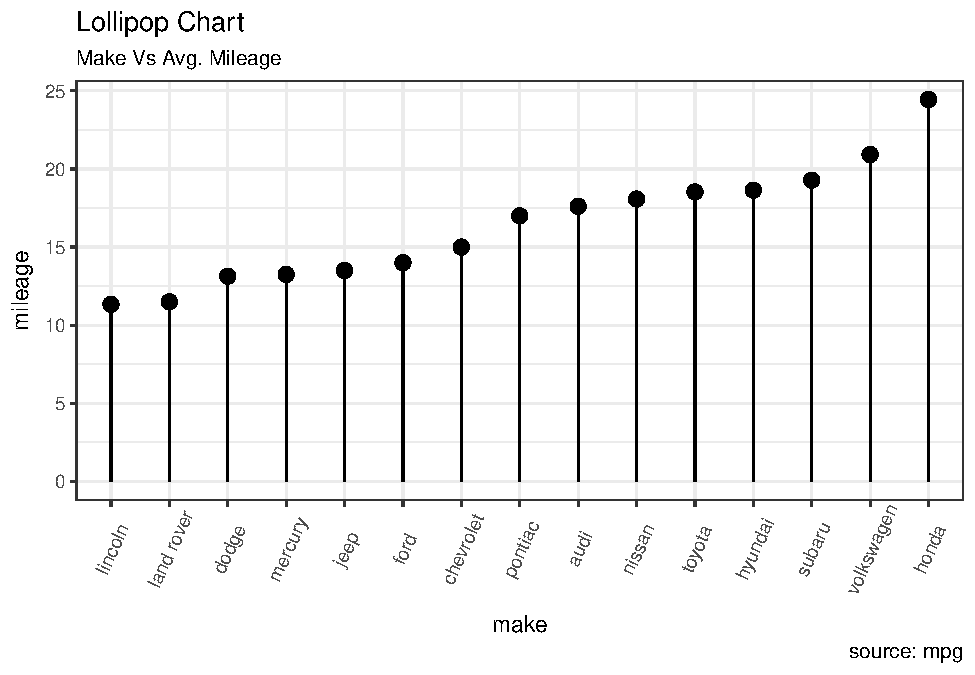
\includegraphics{ggplot2-50examples_files/figure-latex/unnamed-chunk-18-1.pdf}

\newpage

\textbf{Dot Plot}

Dot plots are very similar to lollipops, but without the line and is
flipped to horizontal position. It emphasizes more on the rank ordering
of items with respect to actual values and how far apart are the
entities with respect to each other.

\begin{Shaded}
\begin{Highlighting}[]
\KeywordTok{library}\NormalTok{(ggplot2)}
\KeywordTok{library}\NormalTok{(scales)}
\KeywordTok{theme_set}\NormalTok{(}\KeywordTok{theme_classic}\NormalTok{())}

\CommentTok{# Plot}
\KeywordTok{ggplot}\NormalTok{(cty_mpg, }\KeywordTok{aes}\NormalTok{(}\DataTypeTok{x=}\NormalTok{make, }\DataTypeTok{y=}\NormalTok{mileage)) }\OperatorTok{+}\StringTok{ }
\StringTok{  }\KeywordTok{geom_point}\NormalTok{(}\DataTypeTok{col=}\StringTok{"tomato2"}\NormalTok{, }\DataTypeTok{size=}\DecValTok{3}\NormalTok{) }\OperatorTok{+}\StringTok{   }\CommentTok{# Draw points}
\StringTok{  }\KeywordTok{geom_segment}\NormalTok{(}\KeywordTok{aes}\NormalTok{(}\DataTypeTok{x=}\NormalTok{make, }
                   \DataTypeTok{xend=}\NormalTok{make, }
                   \DataTypeTok{y=}\KeywordTok{min}\NormalTok{(mileage), }
                   \DataTypeTok{yend=}\KeywordTok{max}\NormalTok{(mileage)), }
               \DataTypeTok{linetype=}\StringTok{"dashed"}\NormalTok{, }
               \DataTypeTok{size=}\FloatTok{0.1}\NormalTok{) }\OperatorTok{+}\StringTok{   }\CommentTok{# Draw dashed lines}
\StringTok{  }\KeywordTok{labs}\NormalTok{(}\DataTypeTok{title=}\StringTok{"Dot Plot"}\NormalTok{, }
       \DataTypeTok{subtitle=}\StringTok{"Make Vs Avg. Mileage"}\NormalTok{, }
       \DataTypeTok{caption=}\StringTok{"source: mpg"}\NormalTok{) }\OperatorTok{+}\StringTok{  }
\StringTok{  }\KeywordTok{coord_flip}\NormalTok{()}
\end{Highlighting}
\end{Shaded}

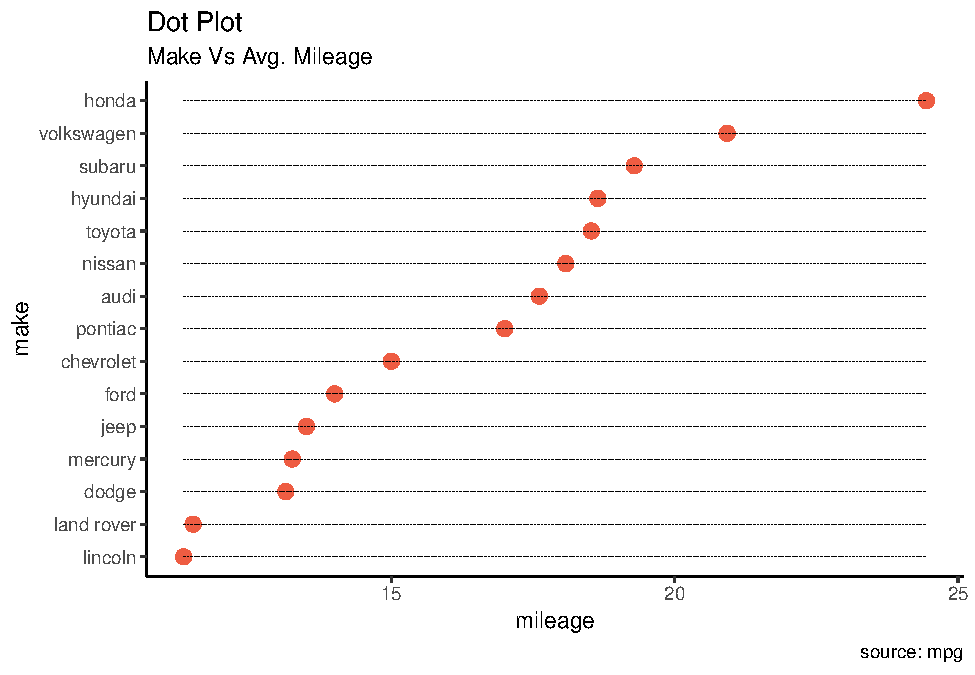
\includegraphics{ggplot2-50examples_files/figure-latex/unnamed-chunk-19-1.pdf}
\newpage

\textbf{Slope Chart}

Slope charts are an excellent way of comparing the positional placements
between 2 points on time. At the moment, there is no builtin function to
construct this. Following code serves as a pointer about how you may
approach this.

\begin{Shaded}
\begin{Highlighting}[]
\KeywordTok{library}\NormalTok{(ggplot2)}
\KeywordTok{library}\NormalTok{(scales)}
\KeywordTok{theme_set}\NormalTok{(}\KeywordTok{theme_classic}\NormalTok{())}

\CommentTok{# prep data}
\NormalTok{df <-}\StringTok{ }\KeywordTok{read.csv}\NormalTok{(}\StringTok{"https://raw.githubusercontent.com/selva86/datasets/master/gdppercap.csv"}\NormalTok{)}
\KeywordTok{colnames}\NormalTok{(df) <-}\StringTok{ }\KeywordTok{c}\NormalTok{(}\StringTok{"continent"}\NormalTok{, }\StringTok{"1952"}\NormalTok{, }\StringTok{"1957"}\NormalTok{)}
\NormalTok{left_label <-}\StringTok{ }\KeywordTok{paste}\NormalTok{(df}\OperatorTok{$}\NormalTok{continent, }\KeywordTok{round}\NormalTok{(df}\OperatorTok{$}\StringTok{`}\DataTypeTok{1952}\StringTok{`}\NormalTok{),}\DataTypeTok{sep=}\StringTok{", "}\NormalTok{)}
\NormalTok{right_label <-}\StringTok{ }\KeywordTok{paste}\NormalTok{(df}\OperatorTok{$}\NormalTok{continent, }\KeywordTok{round}\NormalTok{(df}\OperatorTok{$}\StringTok{`}\DataTypeTok{1957}\StringTok{`}\NormalTok{),}\DataTypeTok{sep=}\StringTok{", "}\NormalTok{)}
\NormalTok{df}\OperatorTok{$}\NormalTok{class <-}\StringTok{ }\KeywordTok{ifelse}\NormalTok{((df}\OperatorTok{$}\StringTok{`}\DataTypeTok{1957}\StringTok{`} \OperatorTok{-}\StringTok{ }\NormalTok{df}\OperatorTok{$}\StringTok{`}\DataTypeTok{1952}\StringTok{`}\NormalTok{) }\OperatorTok{<}\StringTok{ }\DecValTok{0}\NormalTok{, }\StringTok{"red"}\NormalTok{, }\StringTok{"green"}\NormalTok{)}

\CommentTok{# Plot}
\NormalTok{p <-}\StringTok{ }\KeywordTok{ggplot}\NormalTok{(df) }\OperatorTok{+}\StringTok{ }
\StringTok{  }\KeywordTok{geom_segment}\NormalTok{(}\KeywordTok{aes}\NormalTok{(}\DataTypeTok{x=}\DecValTok{1}\NormalTok{, }\DataTypeTok{xend=}\DecValTok{2}\NormalTok{, }\DataTypeTok{y=}\StringTok{`}\DataTypeTok{1952}\StringTok{`}\NormalTok{, }\DataTypeTok{yend=}\StringTok{`}\DataTypeTok{1957}\StringTok{`}\NormalTok{, }\DataTypeTok{col=}\NormalTok{class), }\DataTypeTok{size=}\NormalTok{.}\DecValTok{75}\NormalTok{, }\DataTypeTok{show.legend=}\NormalTok{F) }\OperatorTok{+}\StringTok{ }
\StringTok{  }\KeywordTok{geom_vline}\NormalTok{(}\DataTypeTok{xintercept=}\DecValTok{1}\NormalTok{, }\DataTypeTok{linetype=}\StringTok{"dashed"}\NormalTok{, }\DataTypeTok{size=}\NormalTok{.}\DecValTok{1}\NormalTok{) }\OperatorTok{+}\StringTok{ }
\StringTok{  }\KeywordTok{geom_vline}\NormalTok{(}\DataTypeTok{xintercept=}\DecValTok{2}\NormalTok{, }\DataTypeTok{linetype=}\StringTok{"dashed"}\NormalTok{, }\DataTypeTok{size=}\NormalTok{.}\DecValTok{1}\NormalTok{) }\OperatorTok{+}
\StringTok{  }\KeywordTok{scale_color_manual}\NormalTok{(}\DataTypeTok{labels =} \KeywordTok{c}\NormalTok{(}\StringTok{"Up"}\NormalTok{, }\StringTok{"Down"}\NormalTok{), }
                     \DataTypeTok{values =} \KeywordTok{c}\NormalTok{(}\StringTok{"green"}\NormalTok{=}\StringTok{"#00ba38"}\NormalTok{, }\StringTok{"red"}\NormalTok{=}\StringTok{"#f8766d"}\NormalTok{)) }\OperatorTok{+}\StringTok{  }\CommentTok{# color of lines}
\StringTok{  }\KeywordTok{labs}\NormalTok{(}\DataTypeTok{x=}\StringTok{""}\NormalTok{, }\DataTypeTok{y=}\StringTok{"Mean GdpPerCap"}\NormalTok{) }\OperatorTok{+}\StringTok{  }\CommentTok{# Axis labels}
\StringTok{  }\KeywordTok{xlim}\NormalTok{(.}\DecValTok{5}\NormalTok{, }\FloatTok{2.5}\NormalTok{) }\OperatorTok{+}\StringTok{ }\KeywordTok{ylim}\NormalTok{(}\DecValTok{0}\NormalTok{,(}\FloatTok{1.1}\OperatorTok{*}\NormalTok{(}\KeywordTok{max}\NormalTok{(df}\OperatorTok{$}\StringTok{`}\DataTypeTok{1952}\StringTok{`}\NormalTok{, df}\OperatorTok{$}\StringTok{`}\DataTypeTok{1957}\StringTok{`}\NormalTok{))))  }
\CommentTok{# X and Y axis limits}

\CommentTok{# Add texts}
\NormalTok{p <-}\StringTok{ }\NormalTok{p }\OperatorTok{+}\StringTok{ }
\StringTok{  }\KeywordTok{geom_text}\NormalTok{(}\DataTypeTok{label=}\NormalTok{left_label, }\DataTypeTok{y=}\NormalTok{df}\OperatorTok{$}\StringTok{`}\DataTypeTok{1952}\StringTok{`}\NormalTok{, }\DataTypeTok{x=}\KeywordTok{rep}\NormalTok{(}\DecValTok{1}\NormalTok{, }\KeywordTok{NROW}\NormalTok{(df)), }\DataTypeTok{hjust=}\FloatTok{1.1}\NormalTok{, }\DataTypeTok{size=}\FloatTok{3.5}\NormalTok{)}
\NormalTok{p <-}\StringTok{ }\NormalTok{p }\OperatorTok{+}\StringTok{ }
\StringTok{  }\KeywordTok{geom_text}\NormalTok{(}\DataTypeTok{label=}\NormalTok{right_label, }\DataTypeTok{y=}\NormalTok{df}\OperatorTok{$}\StringTok{`}\DataTypeTok{1957}\StringTok{`}\NormalTok{, }\DataTypeTok{x=}\KeywordTok{rep}\NormalTok{(}\DecValTok{2}\NormalTok{, }\KeywordTok{NROW}\NormalTok{(df)), }\DataTypeTok{hjust=}\OperatorTok{-}\FloatTok{0.1}\NormalTok{, }\DataTypeTok{size=}\FloatTok{3.5}\NormalTok{)}
\NormalTok{p <-}\StringTok{ }\NormalTok{p }\OperatorTok{+}\StringTok{ }
\StringTok{  }\KeywordTok{geom_text}\NormalTok{(}\DataTypeTok{label=}\StringTok{"Time 1"}\NormalTok{, }\DataTypeTok{x=}\DecValTok{1}\NormalTok{, }\DataTypeTok{y=}\FloatTok{1.1}\OperatorTok{*}\NormalTok{(}\KeywordTok{max}\NormalTok{(df}\OperatorTok{$}\StringTok{`}\DataTypeTok{1952}\StringTok{`}\NormalTok{, df}\OperatorTok{$}\StringTok{`}\DataTypeTok{1957}\StringTok{`}\NormalTok{)), }\DataTypeTok{hjust=}\FloatTok{1.2}\NormalTok{, }\DataTypeTok{size=}\DecValTok{5}\NormalTok{)  }\CommentTok{# title}
\NormalTok{p <-}\StringTok{ }\NormalTok{p }\OperatorTok{+}\StringTok{ }
\StringTok{  }\KeywordTok{geom_text}\NormalTok{(}\DataTypeTok{label=}\StringTok{"Time 2"}\NormalTok{, }\DataTypeTok{x=}\DecValTok{2}\NormalTok{, }\DataTypeTok{y=}\FloatTok{1.1}\OperatorTok{*}\NormalTok{(}\KeywordTok{max}\NormalTok{(df}\OperatorTok{$}\StringTok{`}\DataTypeTok{1952}\StringTok{`}\NormalTok{, df}\OperatorTok{$}\StringTok{`}\DataTypeTok{1957}\StringTok{`}\NormalTok{)), }\DataTypeTok{hjust=}\OperatorTok{-}\FloatTok{0.1}\NormalTok{, }\DataTypeTok{size=}\DecValTok{5}\NormalTok{)  }\CommentTok{# title}

\CommentTok{# Minify theme}
\NormalTok{p }\OperatorTok{+}\StringTok{ }\KeywordTok{theme}\NormalTok{(}\DataTypeTok{panel.background =} \KeywordTok{element_blank}\NormalTok{(), }
           \DataTypeTok{panel.grid =} \KeywordTok{element_blank}\NormalTok{(),}
           \DataTypeTok{axis.ticks =} \KeywordTok{element_blank}\NormalTok{(),}
           \DataTypeTok{axis.text.x =} \KeywordTok{element_blank}\NormalTok{(),}
           \DataTypeTok{panel.border =} \KeywordTok{element_blank}\NormalTok{(),}
           \DataTypeTok{plot.margin =} \KeywordTok{unit}\NormalTok{(}\KeywordTok{c}\NormalTok{(}\DecValTok{1}\NormalTok{,}\DecValTok{2}\NormalTok{,}\DecValTok{1}\NormalTok{,}\DecValTok{2}\NormalTok{), }\StringTok{"cm"}\NormalTok{))}
\end{Highlighting}
\end{Shaded}

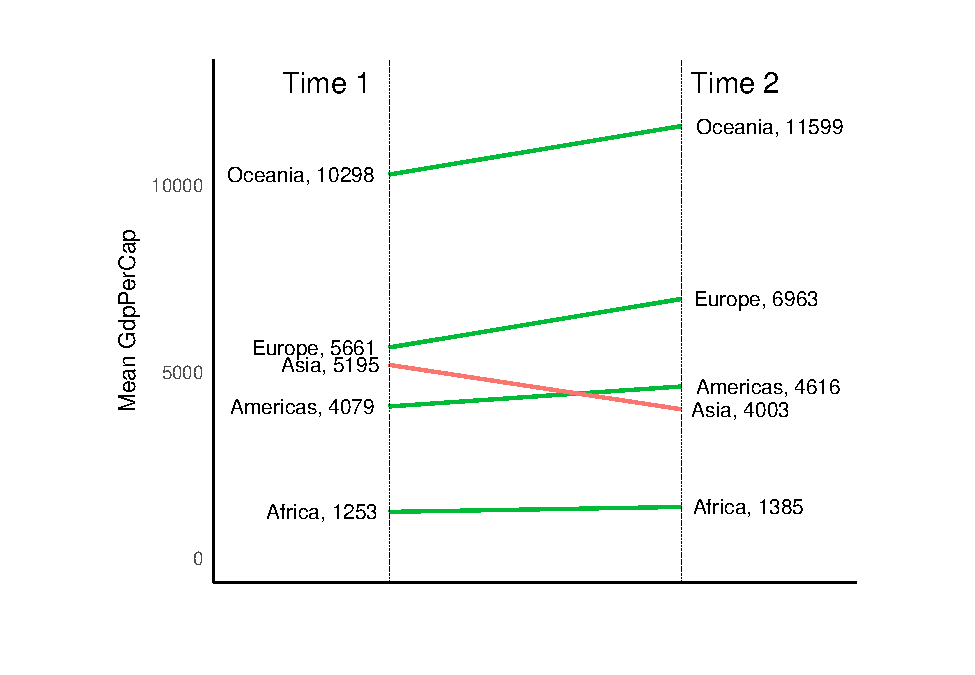
\includegraphics{ggplot2-50examples_files/figure-latex/unnamed-chunk-20-1.pdf}

\newpage

\textbf{Dumbbell Plot}

Dumbbell charts are a great tool if you wish to: 1. Visualize relative
positions (like growth and decline) between two points in time. 2.
Compare distance between two categories.

In order to get the correct ordering of the dumbbells, the Y variable
should be a factor and the levels of the factor variable should be in
the same order as it should appear in the plot.

\begin{Shaded}
\begin{Highlighting}[]
\CommentTok{# devtools::install_github("hrbrmstr/ggalt")}
\KeywordTok{library}\NormalTok{(ggplot2)}
\KeywordTok{library}\NormalTok{(ggalt)}
\KeywordTok{theme_set}\NormalTok{(}\KeywordTok{theme_classic}\NormalTok{())}

\NormalTok{health <-}\StringTok{ }\KeywordTok{read.csv}\NormalTok{(}\StringTok{"https://raw.githubusercontent.com/selva86/datasets/master/health.csv"}\NormalTok{)}
\NormalTok{health}\OperatorTok{$}\NormalTok{Area <-}\StringTok{ }\KeywordTok{factor}\NormalTok{(health}\OperatorTok{$}\NormalTok{Area, }\DataTypeTok{levels=}\KeywordTok{as.character}\NormalTok{(health}\OperatorTok{$}\NormalTok{Area))  }
\CommentTok{# for right ordering of the dumbells}

\CommentTok{# health$Area <- factor(health$Area)}
\NormalTok{gg <-}\StringTok{ }\KeywordTok{ggplot}\NormalTok{(health, }\KeywordTok{aes}\NormalTok{(}\DataTypeTok{x=}\NormalTok{pct_}\DecValTok{2013}\NormalTok{, }\DataTypeTok{xend=}\NormalTok{pct_}\DecValTok{2014}\NormalTok{, }\DataTypeTok{y=}\NormalTok{Area, }\DataTypeTok{group=}\NormalTok{Area)) }\OperatorTok{+}\StringTok{ }
\StringTok{        }\KeywordTok{geom_dumbbell}\NormalTok{(}\DataTypeTok{color=}\StringTok{"#a3c4dc"}\NormalTok{, }
                      \DataTypeTok{size=}\FloatTok{0.75}\NormalTok{, }
                      \DataTypeTok{point.colour.l=}\StringTok{"#0e668b"}\NormalTok{) }\OperatorTok{+}\StringTok{ }
\StringTok{        }\KeywordTok{scale_x_continuous}\NormalTok{(}\DataTypeTok{label=}\NormalTok{percent) }\OperatorTok{+}\StringTok{ }
\StringTok{        }\KeywordTok{labs}\NormalTok{(}\DataTypeTok{x=}\OtherTok{NULL}\NormalTok{, }
             \DataTypeTok{y=}\OtherTok{NULL}\NormalTok{, }
             \DataTypeTok{title=}\StringTok{"Dumbbell Chart"}\NormalTok{, }
             \DataTypeTok{subtitle=}\StringTok{"Pct Change: 2013 vs 2014"}\NormalTok{, }
             \DataTypeTok{caption=}\StringTok{"Source: https://github.com/hrbrmstr/ggalt"}\NormalTok{) }\OperatorTok{+}
\StringTok{        }\KeywordTok{theme}\NormalTok{(}\DataTypeTok{plot.title =} \KeywordTok{element_text}\NormalTok{(}\DataTypeTok{hjust=}\FloatTok{0.5}\NormalTok{, }\DataTypeTok{face=}\StringTok{"bold"}\NormalTok{),}
              \DataTypeTok{plot.background=}\KeywordTok{element_rect}\NormalTok{(}\DataTypeTok{fill=}\StringTok{"#f7f7f7"}\NormalTok{),}
              \DataTypeTok{panel.background=}\KeywordTok{element_rect}\NormalTok{(}\DataTypeTok{fill=}\StringTok{"#f7f7f7"}\NormalTok{),}
              \DataTypeTok{panel.grid.minor=}\KeywordTok{element_blank}\NormalTok{(),}
              \DataTypeTok{panel.grid.major.y=}\KeywordTok{element_blank}\NormalTok{(),}
              \DataTypeTok{panel.grid.major.x=}\KeywordTok{element_line}\NormalTok{(),}
              \DataTypeTok{axis.ticks=}\KeywordTok{element_blank}\NormalTok{(),}
              \DataTypeTok{legend.position=}\StringTok{"top"}\NormalTok{,}
              \DataTypeTok{panel.border=}\KeywordTok{element_blank}\NormalTok{())}
\end{Highlighting}
\end{Shaded}

\begin{verbatim}
## Warning: Ignoring unknown parameters: point.colour.l
\end{verbatim}

\begin{Shaded}
\begin{Highlighting}[]
\KeywordTok{plot}\NormalTok{(gg)}
\end{Highlighting}
\end{Shaded}

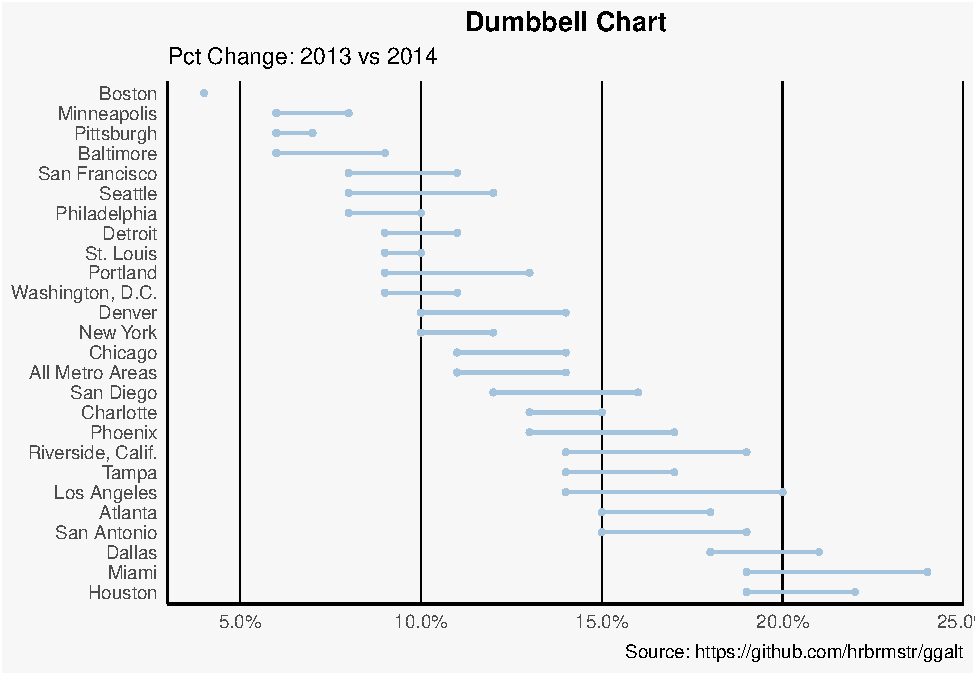
\includegraphics{ggplot2-50examples_files/figure-latex/unnamed-chunk-21-1.pdf}

\newpage

\subsection{4. Distribution}\label{distribution}

When you have lots and lots of data points and want to study where and
how the data points are distributed.

\textbf{Histogram}

By default, if only one variable is supplied, the \texttt{geom\_bar()}
tries to calculate the count. In order for it to behave like a bar
chart, the stat=identity option has to be set and x and y values must be
provided.

\textbf{Histogram on a continuous variable}

Histogram on a continuous variable can be accomplished using either
\texttt{geom\_bar()} or \texttt{geom\_histogram()}. When using
\texttt{geom\_histogram()}, you can control the number of bars using the
bins option. Else, you can set the range covered by each bin using
binwidth. The value of binwidth is on the same scale as the continuous
variable on which histogram is built. Since, geom\_histogram gives
facility to control both number of bins as well as binwidth, it is the
preferred option to create histogram on continuous variables.

\begin{Shaded}
\begin{Highlighting}[]
\KeywordTok{library}\NormalTok{(ggplot2)}
\KeywordTok{theme_set}\NormalTok{(}\KeywordTok{theme_classic}\NormalTok{())}

\CommentTok{# Histogram on a Continuous (Numeric) Variable}
\NormalTok{g <-}\StringTok{ }\KeywordTok{ggplot}\NormalTok{(mpg, }\KeywordTok{aes}\NormalTok{(displ)) }\OperatorTok{+}\StringTok{ }\KeywordTok{scale_fill_brewer}\NormalTok{(}\DataTypeTok{palette =} \StringTok{"Spectral"}\NormalTok{)}

\NormalTok{g }\OperatorTok{+}\StringTok{ }\KeywordTok{geom_histogram}\NormalTok{(}\KeywordTok{aes}\NormalTok{(}\DataTypeTok{fill=}\NormalTok{class), }
                   \DataTypeTok{binwidth =}\NormalTok{ .}\DecValTok{1}\NormalTok{, }
                   \DataTypeTok{col=}\StringTok{"black"}\NormalTok{, }
                   \DataTypeTok{size=}\NormalTok{.}\DecValTok{1}\NormalTok{) }\OperatorTok{+}\StringTok{  }\CommentTok{# change binwidth}
\StringTok{  }\KeywordTok{labs}\NormalTok{(}\DataTypeTok{title=}\StringTok{"Histogram with Auto Binning"}\NormalTok{, }
       \DataTypeTok{subtitle=}\StringTok{"Engine Displacement across Vehicle Classes"}\NormalTok{)  }
\end{Highlighting}
\end{Shaded}

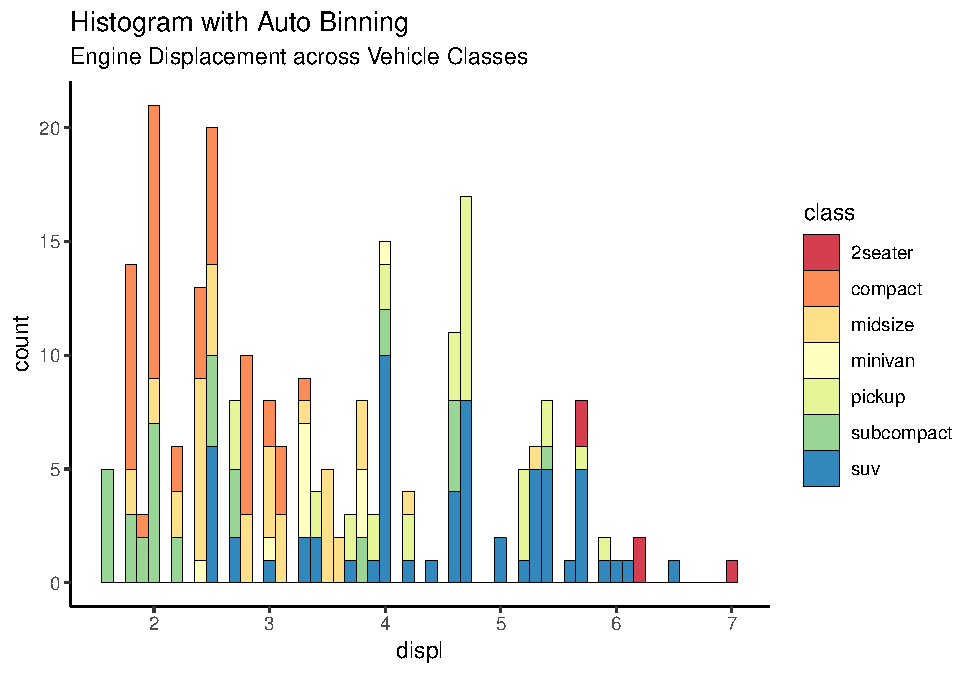
\includegraphics{ggplot2-50examples_files/figure-latex/unnamed-chunk-22-1.pdf}

\begin{Shaded}
\begin{Highlighting}[]
\NormalTok{g }\OperatorTok{+}\StringTok{ }\KeywordTok{geom_histogram}\NormalTok{(}\KeywordTok{aes}\NormalTok{(}\DataTypeTok{fill=}\NormalTok{class), }
                   \DataTypeTok{bins=}\DecValTok{5}\NormalTok{, }
                   \DataTypeTok{col=}\StringTok{"black"}\NormalTok{, }
                   \DataTypeTok{size=}\NormalTok{.}\DecValTok{1}\NormalTok{) }\OperatorTok{+}\StringTok{   }\CommentTok{# change number of bins}
\StringTok{  }\KeywordTok{labs}\NormalTok{(}\DataTypeTok{title=}\StringTok{"Histogram with Fixed Bins"}\NormalTok{, }
       \DataTypeTok{subtitle=}\StringTok{"Engine Displacement across Vehicle Classes"}\NormalTok{) }
\end{Highlighting}
\end{Shaded}

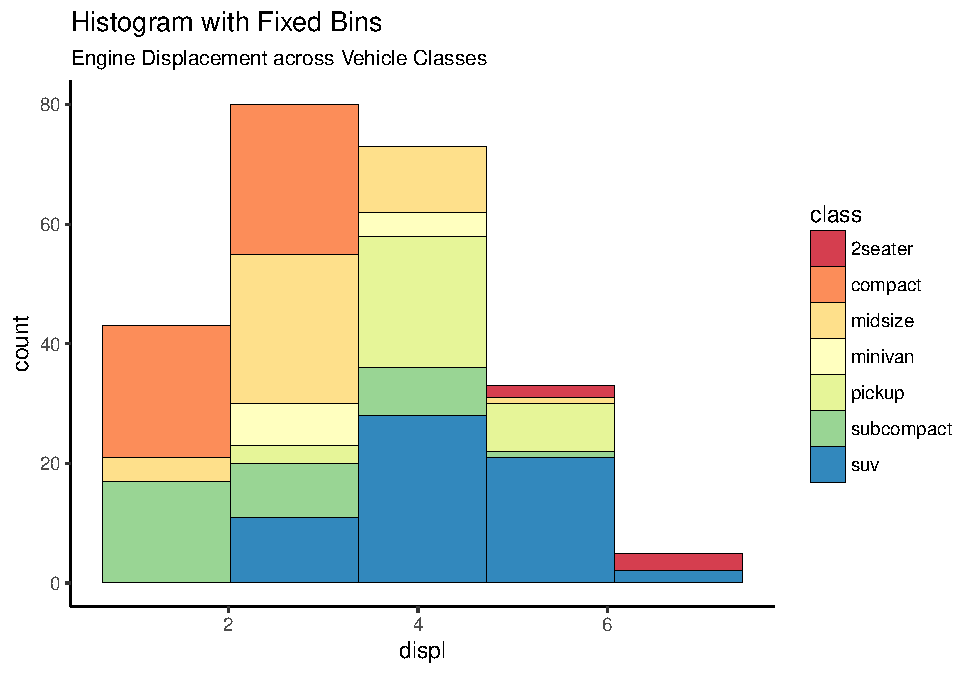
\includegraphics{ggplot2-50examples_files/figure-latex/unnamed-chunk-22-2.pdf}

\newpage

\textbf{Histogram on a categorical variable}

Histogram on a categorical variable would result in a frequency chart
showing bars for each category. By adjusting width, you can adjust the
thickness of the bars.

\begin{Shaded}
\begin{Highlighting}[]
\KeywordTok{library}\NormalTok{(ggplot2)}
\KeywordTok{theme_set}\NormalTok{(}\KeywordTok{theme_classic}\NormalTok{())}

\CommentTok{# Histogram on a Categorical variable}
\NormalTok{g <-}\StringTok{ }\KeywordTok{ggplot}\NormalTok{(mpg, }\KeywordTok{aes}\NormalTok{(manufacturer))}
\NormalTok{g }\OperatorTok{+}\StringTok{ }\KeywordTok{geom_bar}\NormalTok{(}\KeywordTok{aes}\NormalTok{(}\DataTypeTok{fill=}\NormalTok{class), }\DataTypeTok{width =} \FloatTok{0.5}\NormalTok{) }\OperatorTok{+}\StringTok{ }
\StringTok{  }\KeywordTok{theme}\NormalTok{(}\DataTypeTok{axis.text.x =} \KeywordTok{element_text}\NormalTok{(}\DataTypeTok{angle=}\DecValTok{65}\NormalTok{, }\DataTypeTok{vjust=}\FloatTok{0.6}\NormalTok{)) }\OperatorTok{+}\StringTok{ }
\StringTok{  }\KeywordTok{labs}\NormalTok{(}\DataTypeTok{title=}\StringTok{"Histogram on Categorical Variable"}\NormalTok{, }
       \DataTypeTok{subtitle=}\StringTok{"Manufacturer across Vehicle Classes"}\NormalTok{) }
\end{Highlighting}
\end{Shaded}

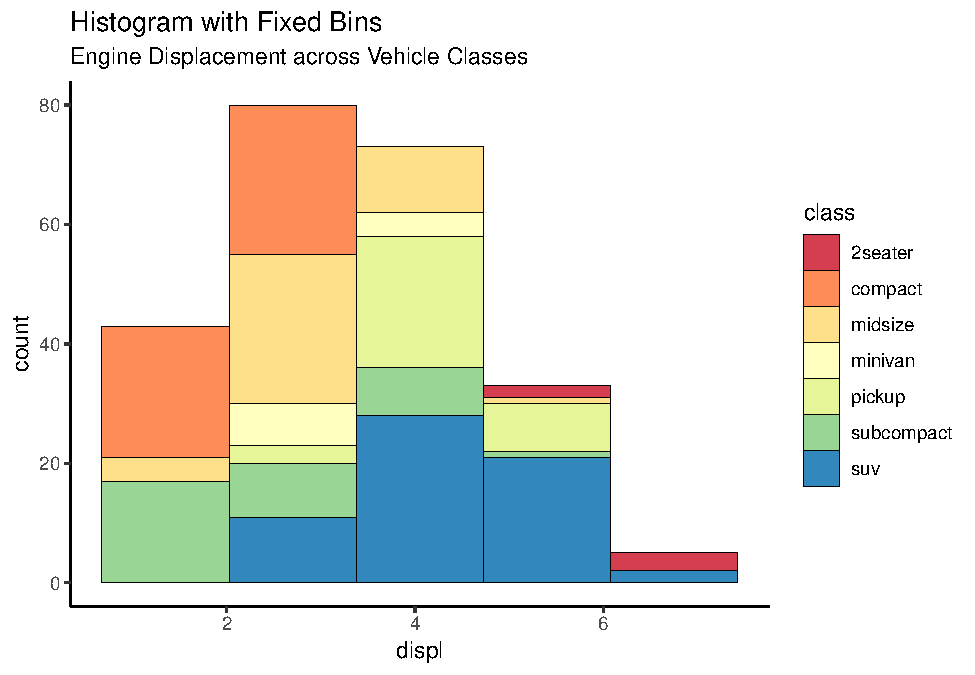
\includegraphics{ggplot2-50examples_files/figure-latex/unnamed-chunk-23-1.pdf}

\newpage

\textbf{Density plot}

\begin{Shaded}
\begin{Highlighting}[]
\KeywordTok{library}\NormalTok{(ggplot2)}
\KeywordTok{theme_set}\NormalTok{(}\KeywordTok{theme_classic}\NormalTok{())}

\CommentTok{# Plot}
\NormalTok{g <-}\StringTok{ }\KeywordTok{ggplot}\NormalTok{(mpg, }\KeywordTok{aes}\NormalTok{(cty))}
\NormalTok{g }\OperatorTok{+}\StringTok{ }\KeywordTok{geom_density}\NormalTok{(}\KeywordTok{aes}\NormalTok{(}\DataTypeTok{fill=}\KeywordTok{factor}\NormalTok{(cyl)), }\DataTypeTok{alpha=}\FloatTok{0.8}\NormalTok{) }\OperatorTok{+}\StringTok{ }
\StringTok{    }\KeywordTok{labs}\NormalTok{(}\DataTypeTok{title=}\StringTok{"Density plot"}\NormalTok{, }
         \DataTypeTok{subtitle=}\StringTok{"City Mileage Grouped by Number of cylinders"}\NormalTok{,}
         \DataTypeTok{caption=}\StringTok{"Source: mpg"}\NormalTok{,}
         \DataTypeTok{x=}\StringTok{"City Mileage"}\NormalTok{,}
         \DataTypeTok{fill=}\StringTok{"# Cylinders"}\NormalTok{)}
\end{Highlighting}
\end{Shaded}

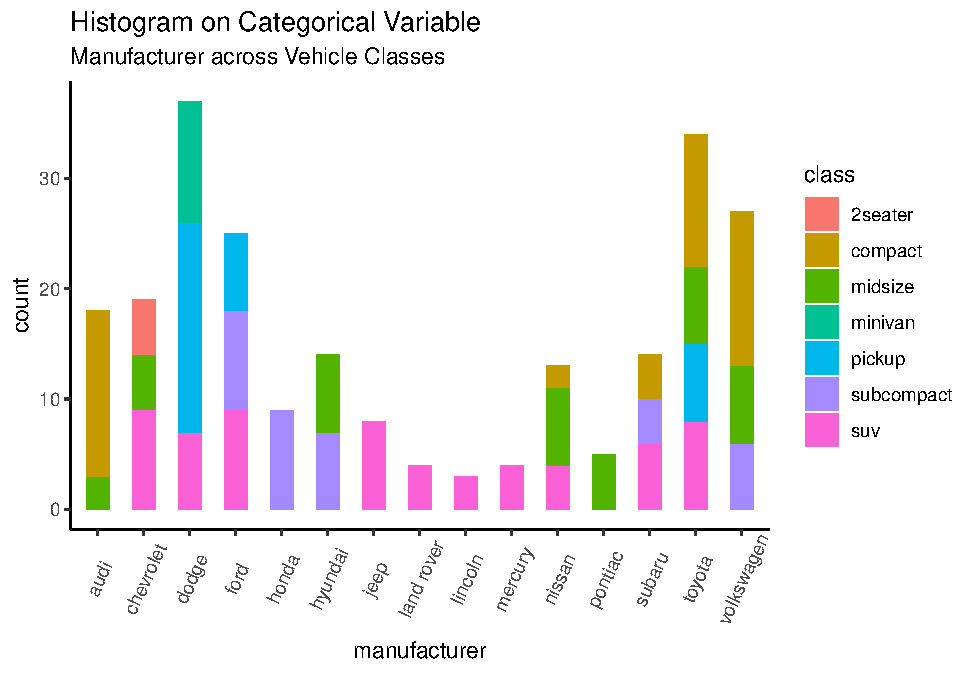
\includegraphics{ggplot2-50examples_files/figure-latex/unnamed-chunk-24-1.pdf}
\newpage

\textbf{Box Plot}

Box plot is an excellent tool to study the distribution. It can also
show the distributions within multiple groups, along with the median,
range and outliers if any.

The dark line inside the box represents the median. The top of box is
75\%ile and bottom of box is 25\%ile. The end points of the lines (aka
whiskers) is at a distance of 1.5*IQR, where IQR or Inter Quartile Range
is the distance between 25th and 75th percentiles. The points outside
the whiskers are marked as dots and are normally considered as extreme
points.

Setting \texttt{varwidth=T} adjusts the width of the boxes to be
proportional to the number of observation it contains.

\begin{Shaded}
\begin{Highlighting}[]
\KeywordTok{library}\NormalTok{(ggplot2)}
\KeywordTok{theme_set}\NormalTok{(}\KeywordTok{theme_classic}\NormalTok{())}

\CommentTok{# Plot}
\NormalTok{g <-}\StringTok{ }\KeywordTok{ggplot}\NormalTok{(mpg, }\KeywordTok{aes}\NormalTok{(class, cty))}
\NormalTok{g }\OperatorTok{+}\StringTok{ }\KeywordTok{geom_boxplot}\NormalTok{(}\DataTypeTok{varwidth=}\NormalTok{T, }\DataTypeTok{fill=}\StringTok{"plum"}\NormalTok{) }\OperatorTok{+}\StringTok{ }
\StringTok{    }\KeywordTok{labs}\NormalTok{(}\DataTypeTok{title=}\StringTok{"Box plot"}\NormalTok{, }
         \DataTypeTok{subtitle=}\StringTok{"City Mileage grouped by Class of vehicle"}\NormalTok{,}
         \DataTypeTok{caption=}\StringTok{"Source: mpg"}\NormalTok{,}
         \DataTypeTok{x=}\StringTok{"Class of Vehicle"}\NormalTok{,}
         \DataTypeTok{y=}\StringTok{"City Mileage"}\NormalTok{)}
\end{Highlighting}
\end{Shaded}

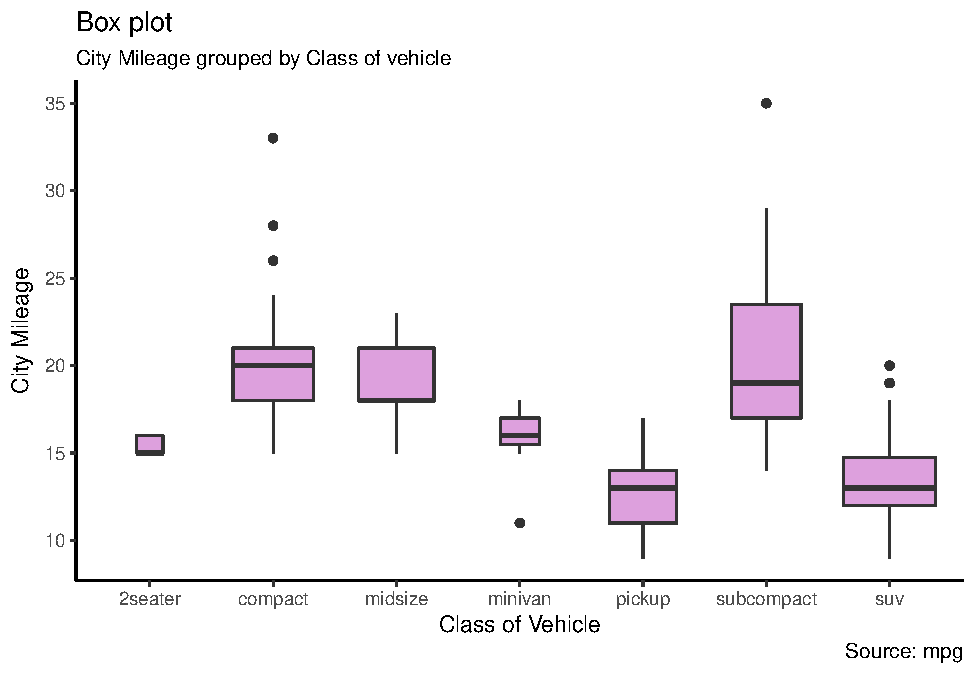
\includegraphics{ggplot2-50examples_files/figure-latex/unnamed-chunk-25-1.pdf}

\begin{Shaded}
\begin{Highlighting}[]
\KeywordTok{library}\NormalTok{(ggthemes)}
\NormalTok{g <-}\StringTok{ }\KeywordTok{ggplot}\NormalTok{(mpg, }\KeywordTok{aes}\NormalTok{(class, cty))}
\NormalTok{g }\OperatorTok{+}\StringTok{ }\KeywordTok{geom_boxplot}\NormalTok{(}\KeywordTok{aes}\NormalTok{(}\DataTypeTok{fill=}\KeywordTok{factor}\NormalTok{(cyl))) }\OperatorTok{+}\StringTok{ }
\StringTok{  }\KeywordTok{theme}\NormalTok{(}\DataTypeTok{axis.text.x =} \KeywordTok{element_text}\NormalTok{(}\DataTypeTok{angle=}\DecValTok{65}\NormalTok{, }\DataTypeTok{vjust=}\FloatTok{0.6}\NormalTok{)) }\OperatorTok{+}\StringTok{ }
\StringTok{  }\KeywordTok{labs}\NormalTok{(}\DataTypeTok{title=}\StringTok{"Box plot"}\NormalTok{, }
       \DataTypeTok{subtitle=}\StringTok{"City Mileage grouped by Class of vehicle"}\NormalTok{,}
       \DataTypeTok{caption=}\StringTok{"Source: mpg"}\NormalTok{,}
       \DataTypeTok{x=}\StringTok{"Class of Vehicle"}\NormalTok{,}
       \DataTypeTok{y=}\StringTok{"City Mileage"}\NormalTok{)}
\end{Highlighting}
\end{Shaded}

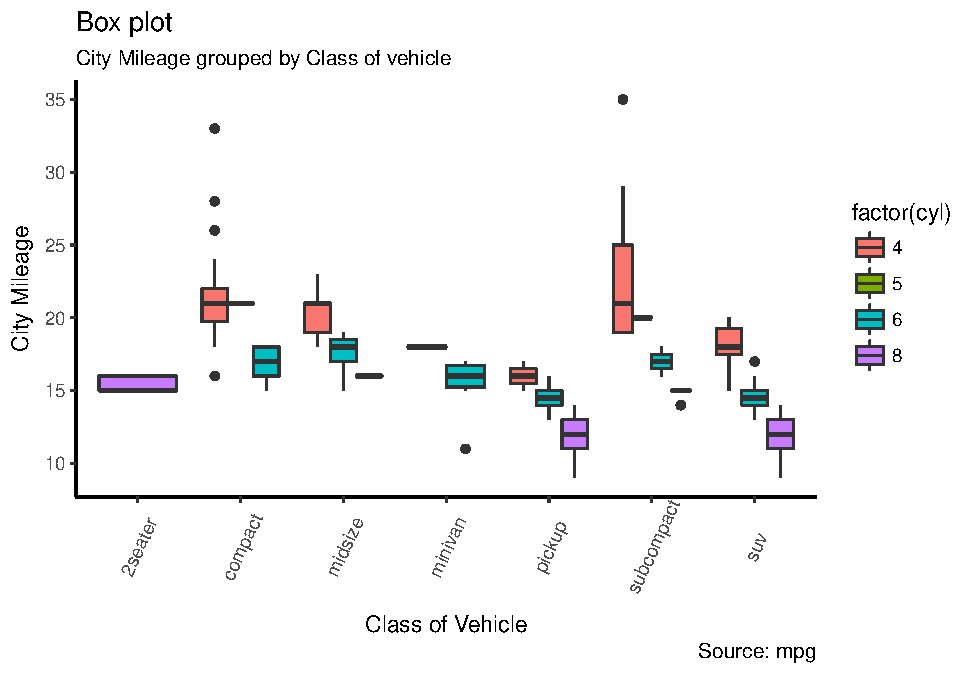
\includegraphics{ggplot2-50examples_files/figure-latex/unnamed-chunk-25-2.pdf}
\newpage

\textbf{Dot + Box Plot}

On top of the information provided by a box plot, the dot plot can
provide more clear information in the form of summary statistics by each
group. The dots are staggered such that each dot represents one
observation. So, in below chart, the number of dots for a given
manufacturer will match the number of rows of that manufacturer in
source data.

\begin{Shaded}
\begin{Highlighting}[]
\KeywordTok{library}\NormalTok{(ggplot2)}
\KeywordTok{theme_set}\NormalTok{(}\KeywordTok{theme_bw}\NormalTok{())}

\CommentTok{# plot}
\NormalTok{g <-}\StringTok{ }\KeywordTok{ggplot}\NormalTok{(mpg, }\KeywordTok{aes}\NormalTok{(manufacturer, cty))}
\NormalTok{g }\OperatorTok{+}\StringTok{ }\KeywordTok{geom_boxplot}\NormalTok{() }\OperatorTok{+}\StringTok{ }
\StringTok{  }\KeywordTok{geom_dotplot}\NormalTok{(}\DataTypeTok{binaxis=}\StringTok{'y'}\NormalTok{, }
               \DataTypeTok{stackdir=}\StringTok{'center'}\NormalTok{, }
               \DataTypeTok{dotsize =}\NormalTok{ .}\DecValTok{5}\NormalTok{, }
               \DataTypeTok{fill=}\StringTok{"red"}\NormalTok{) }\OperatorTok{+}
\StringTok{  }\KeywordTok{theme}\NormalTok{(}\DataTypeTok{axis.text.x =} \KeywordTok{element_text}\NormalTok{(}\DataTypeTok{angle=}\DecValTok{65}\NormalTok{, }\DataTypeTok{vjust=}\FloatTok{0.6}\NormalTok{)) }\OperatorTok{+}\StringTok{ }
\StringTok{  }\KeywordTok{labs}\NormalTok{(}\DataTypeTok{title=}\StringTok{"Box plot + Dot plot"}\NormalTok{, }
       \DataTypeTok{subtitle=}\StringTok{"City Mileage vs Class: Each dot represents 1 row in source data"}\NormalTok{,}
       \DataTypeTok{caption=}\StringTok{"Source: mpg"}\NormalTok{,}
       \DataTypeTok{x=}\StringTok{"Class of Vehicle"}\NormalTok{,}
       \DataTypeTok{y=}\StringTok{"City Mileage"}\NormalTok{)}
\end{Highlighting}
\end{Shaded}

\begin{verbatim}
## `stat_bindot()` using `bins = 30`. Pick better value with `binwidth`.
\end{verbatim}

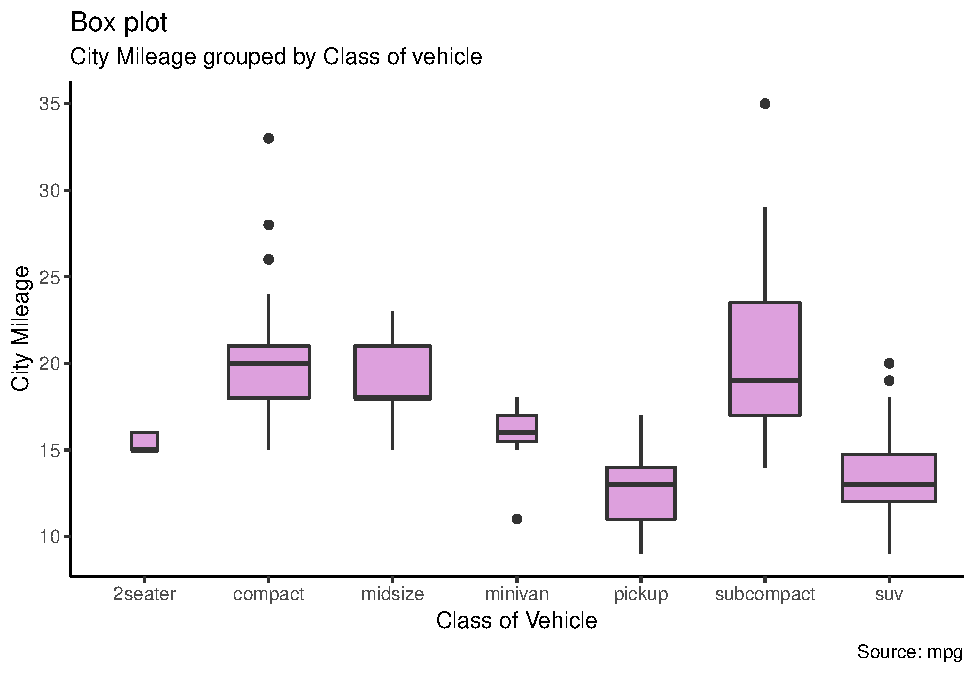
\includegraphics{ggplot2-50examples_files/figure-latex/unnamed-chunk-26-1.pdf}

\newpage

\textbf{Tufte Boxplot}

Tufte box plot, provided by ggthemes package is inspired by the works of
Edward Tufte. Tufte's Box plot is just a box plot made minimal and
visually appealing.

\begin{Shaded}
\begin{Highlighting}[]
\KeywordTok{library}\NormalTok{(ggthemes)}
\KeywordTok{library}\NormalTok{(ggplot2)}
\KeywordTok{theme_set}\NormalTok{(}\KeywordTok{theme_tufte}\NormalTok{())  }\CommentTok{# from ggthemes}

\CommentTok{# plot}
\NormalTok{g <-}\StringTok{ }\KeywordTok{ggplot}\NormalTok{(mpg, }\KeywordTok{aes}\NormalTok{(manufacturer, cty))}
\NormalTok{g }\OperatorTok{+}\StringTok{ }\KeywordTok{geom_tufteboxplot}\NormalTok{() }\OperatorTok{+}\StringTok{ }
\StringTok{      }\KeywordTok{theme}\NormalTok{(}\DataTypeTok{axis.text.x =} \KeywordTok{element_text}\NormalTok{(}\DataTypeTok{angle=}\DecValTok{65}\NormalTok{, }\DataTypeTok{vjust=}\FloatTok{0.6}\NormalTok{)) }\OperatorTok{+}\StringTok{ }
\StringTok{      }\KeywordTok{labs}\NormalTok{(}\DataTypeTok{title=}\StringTok{"Tufte Styled Boxplot"}\NormalTok{, }
           \DataTypeTok{subtitle=}\StringTok{"City Mileage grouped by Class of vehicle"}\NormalTok{,}
           \DataTypeTok{caption=}\StringTok{"Source: mpg"}\NormalTok{,}
           \DataTypeTok{x=}\StringTok{"Class of Vehicle"}\NormalTok{,}
           \DataTypeTok{y=}\StringTok{"City Mileage"}\NormalTok{)}
\end{Highlighting}
\end{Shaded}

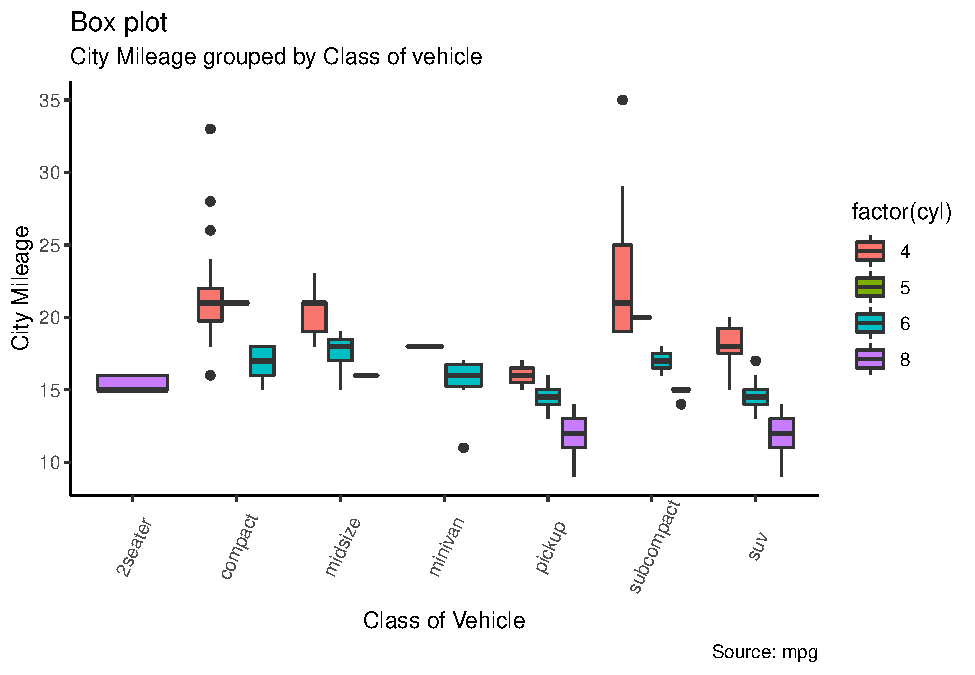
\includegraphics{ggplot2-50examples_files/figure-latex/unnamed-chunk-27-1.pdf}

\newpage

\textbf{Violin Plot}

A violin plot is similar to box plot but shows the density within
groups. Not much info provided as in boxplots. It can be drawn using
geom\_violin().

\begin{Shaded}
\begin{Highlighting}[]
\KeywordTok{library}\NormalTok{(ggplot2)}
\KeywordTok{theme_set}\NormalTok{(}\KeywordTok{theme_bw}\NormalTok{())}

\CommentTok{# plot}
\NormalTok{g <-}\StringTok{ }\KeywordTok{ggplot}\NormalTok{(mpg, }\KeywordTok{aes}\NormalTok{(class, cty))}
\NormalTok{g }\OperatorTok{+}\StringTok{ }\KeywordTok{geom_violin}\NormalTok{() }\OperatorTok{+}\StringTok{ }
\StringTok{  }\KeywordTok{labs}\NormalTok{(}\DataTypeTok{title=}\StringTok{"Violin plot"}\NormalTok{, }
       \DataTypeTok{subtitle=}\StringTok{"City Mileage vs Class of vehicle"}\NormalTok{,}
       \DataTypeTok{caption=}\StringTok{"Source: mpg"}\NormalTok{,}
       \DataTypeTok{x=}\StringTok{"Class of Vehicle"}\NormalTok{,}
       \DataTypeTok{y=}\StringTok{"City Mileage"}\NormalTok{)}
\end{Highlighting}
\end{Shaded}

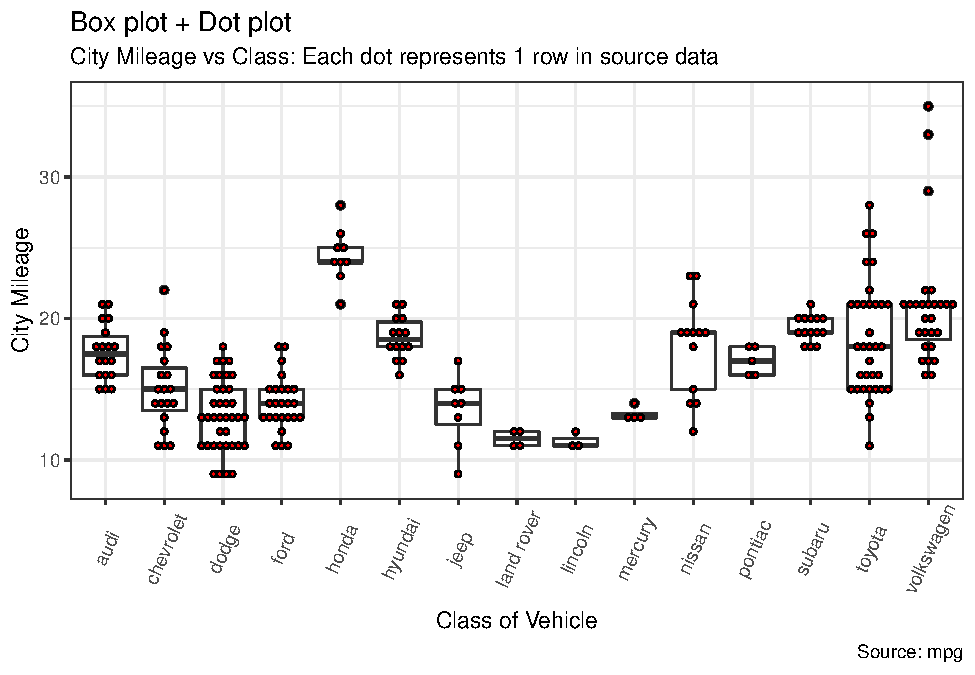
\includegraphics{ggplot2-50examples_files/figure-latex/unnamed-chunk-28-1.pdf}

\newpage

\textbf{Population Pyramid}

Population pyramids offer a unique way of visualizing how much
population or what percentage of population fall under a certain
category. The below pyramid is an excellent example of how many users
are retained at each stage of a email marketing campaign funnel.

\begin{Shaded}
\begin{Highlighting}[]
\KeywordTok{library}\NormalTok{(ggplot2)}
\KeywordTok{library}\NormalTok{(ggthemes)}
\KeywordTok{options}\NormalTok{(}\DataTypeTok{scipen =} \DecValTok{999}\NormalTok{)  }\CommentTok{# turns of scientific notations like 1e+40}

\CommentTok{# Read data}
\NormalTok{email_campaign_funnel <-}
\StringTok{  }\KeywordTok{read.csv}\NormalTok{(}\StringTok{"https://raw.githubusercontent.com/selva86/datasets/master/email_campaign_funnel.csv"}\NormalTok{)}

\CommentTok{# X Axis Breaks and Labels }
\NormalTok{brks <-}\StringTok{ }\KeywordTok{seq}\NormalTok{(}\OperatorTok{-}\DecValTok{15000000}\NormalTok{, }\DecValTok{15000000}\NormalTok{, }\DecValTok{5000000}\NormalTok{)}
\NormalTok{lbls =}\StringTok{ }\KeywordTok{paste0}\NormalTok{(}\KeywordTok{as.character}\NormalTok{(}\KeywordTok{c}\NormalTok{(}\KeywordTok{seq}\NormalTok{(}\DecValTok{15}\NormalTok{, }\DecValTok{0}\NormalTok{, }\OperatorTok{-}\DecValTok{5}\NormalTok{), }\KeywordTok{seq}\NormalTok{(}\DecValTok{5}\NormalTok{, }\DecValTok{15}\NormalTok{, }\DecValTok{5}\NormalTok{))), }\StringTok{"m"}\NormalTok{)}

\CommentTok{# Plot}
\KeywordTok{ggplot}\NormalTok{(email_campaign_funnel, }\KeywordTok{aes}\NormalTok{(}\DataTypeTok{x =}\NormalTok{ Stage, }\DataTypeTok{y =}\NormalTok{ Users, }\DataTypeTok{fill =}\NormalTok{ Gender)) }\OperatorTok{+}\StringTok{   }\CommentTok{# Fill column}
\StringTok{                              }\KeywordTok{geom_bar}\NormalTok{(}\DataTypeTok{stat =} \StringTok{"identity"}\NormalTok{, }\DataTypeTok{width =}\NormalTok{ .}\DecValTok{6}\NormalTok{) }\OperatorTok{+}\StringTok{   }\CommentTok{# draw the bars}
\StringTok{                              }\KeywordTok{scale_y_continuous}\NormalTok{(}\DataTypeTok{breaks =}\NormalTok{ brks,   }\CommentTok{# Breaks}
                                                 \DataTypeTok{labels =}\NormalTok{ lbls) }\OperatorTok{+}\StringTok{ }\CommentTok{# Labels}
\StringTok{                              }\KeywordTok{coord_flip}\NormalTok{() }\OperatorTok{+}\StringTok{  }\CommentTok{# Flip axes}
\StringTok{                              }\KeywordTok{labs}\NormalTok{(}\DataTypeTok{title=}\StringTok{"Email Campaign Funnel"}\NormalTok{) }\OperatorTok{+}
\StringTok{                              }\KeywordTok{theme_tufte}\NormalTok{() }\OperatorTok{+}\StringTok{  }\CommentTok{# Tufte theme from ggfortify}
\StringTok{                              }\KeywordTok{theme}\NormalTok{(}\DataTypeTok{plot.title =} \KeywordTok{element_text}\NormalTok{(}\DataTypeTok{hjust =}\NormalTok{ .}\DecValTok{5}\NormalTok{), }
                                    \DataTypeTok{axis.ticks =} \KeywordTok{element_blank}\NormalTok{()) }\OperatorTok{+}\StringTok{   }\CommentTok{# Centre plot title}
\StringTok{                              }\KeywordTok{scale_fill_brewer}\NormalTok{(}\DataTypeTok{palette =} \StringTok{"Dark2"}\NormalTok{)  }\CommentTok{# Color palette}
\end{Highlighting}
\end{Shaded}

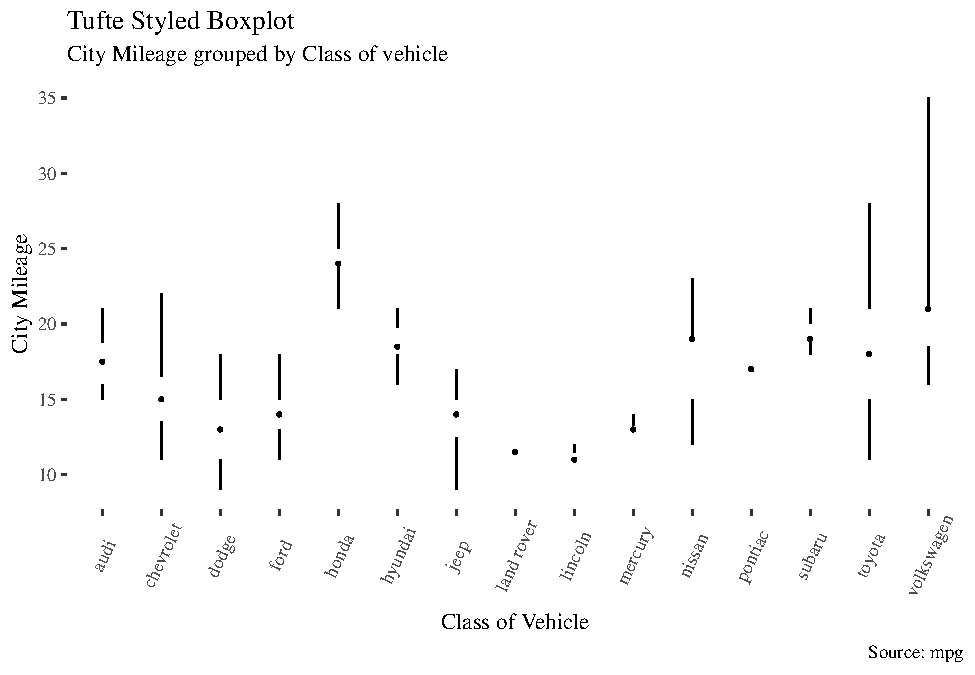
\includegraphics{ggplot2-50examples_files/figure-latex/unnamed-chunk-29-1.pdf}

\newpage

\subsection{5. Composition}\label{composition}

\textbf{Waffle Chart}

Waffle charts is a nice way of showing the categorical composition of
the total population. Though there is no direct function, it can be
articulated by smartly maneuvering the ggplot2 using geom\_tile()
function. The below template should help you create your own waffle.

\begin{Shaded}
\begin{Highlighting}[]
\NormalTok{var <-}\StringTok{ }\NormalTok{mpg}\OperatorTok{$}\NormalTok{class  }\CommentTok{# the categorical data }

\NormalTok{## Prep data (nothing to change here)}
\NormalTok{nrows <-}\StringTok{ }\DecValTok{10}
\NormalTok{df <-}\StringTok{ }\KeywordTok{expand.grid}\NormalTok{(}\DataTypeTok{y =} \DecValTok{1}\OperatorTok{:}\NormalTok{nrows, }\DataTypeTok{x =} \DecValTok{1}\OperatorTok{:}\NormalTok{nrows)}
\NormalTok{categ_table <-}\StringTok{ }\KeywordTok{round}\NormalTok{(}\KeywordTok{table}\NormalTok{(var) }\OperatorTok{*}\StringTok{ }\NormalTok{((nrows}\OperatorTok{*}\NormalTok{nrows)}\OperatorTok{/}\NormalTok{(}\KeywordTok{length}\NormalTok{(var))))}
\NormalTok{categ_table}
\end{Highlighting}
\end{Shaded}

\begin{verbatim}
## var
##    2seater    compact    midsize    minivan     pickup subcompact 
##          2         20         18          5         14         15 
##        suv 
##         26
\end{verbatim}

\begin{Shaded}
\begin{Highlighting}[]
\CommentTok{#>   2seater    compact    midsize    minivan     pickup subcompact        suv }
\CommentTok{#>         2         20         18          5         14         15         26 }

\NormalTok{df}\OperatorTok{$}\NormalTok{category <-}\StringTok{ }\KeywordTok{factor}\NormalTok{(}\KeywordTok{rep}\NormalTok{(}\KeywordTok{names}\NormalTok{(categ_table), categ_table))  }
\CommentTok{# }\AlertTok{NOTE}\CommentTok{: if sum(categ_table) is not 100 (i.e. nrows^2), }
\CommentTok{#       it will need adjustment to make the sum to 100.}

\NormalTok{## Plot}
\KeywordTok{ggplot}\NormalTok{(df, }\KeywordTok{aes}\NormalTok{(}\DataTypeTok{x =}\NormalTok{ x, }\DataTypeTok{y =}\NormalTok{ y, }\DataTypeTok{fill =}\NormalTok{ category)) }\OperatorTok{+}\StringTok{ }
\StringTok{        }\KeywordTok{geom_tile}\NormalTok{(}\DataTypeTok{color =} \StringTok{"black"}\NormalTok{, }\DataTypeTok{size =} \FloatTok{0.5}\NormalTok{) }\OperatorTok{+}
\StringTok{        }\KeywordTok{scale_x_continuous}\NormalTok{(}\DataTypeTok{expand =} \KeywordTok{c}\NormalTok{(}\DecValTok{0}\NormalTok{, }\DecValTok{0}\NormalTok{)) }\OperatorTok{+}
\StringTok{        }\KeywordTok{scale_y_continuous}\NormalTok{(}\DataTypeTok{expand =} \KeywordTok{c}\NormalTok{(}\DecValTok{0}\NormalTok{, }\DecValTok{0}\NormalTok{), }\DataTypeTok{trans =} \StringTok{'reverse'}\NormalTok{) }\OperatorTok{+}
\StringTok{        }\KeywordTok{scale_fill_brewer}\NormalTok{(}\DataTypeTok{palette =} \StringTok{"Set3"}\NormalTok{) }\OperatorTok{+}
\StringTok{        }\KeywordTok{labs}\NormalTok{(}\DataTypeTok{title=}\StringTok{"Waffle Chart"}\NormalTok{, }\DataTypeTok{subtitle=}\StringTok{"'Class' of vehicles"}\NormalTok{,}
             \DataTypeTok{caption=}\StringTok{"Source: mpg"}\NormalTok{) }\OperatorTok{+}\StringTok{ }
\StringTok{        }\KeywordTok{theme}\NormalTok{(}\DataTypeTok{panel.border =} \KeywordTok{element_rect}\NormalTok{(}\DataTypeTok{size =} \DecValTok{2}\NormalTok{),}
              \DataTypeTok{plot.title =} \KeywordTok{element_text}\NormalTok{(}\DataTypeTok{size =} \KeywordTok{rel}\NormalTok{(}\FloatTok{1.2}\NormalTok{)),}
              \DataTypeTok{axis.text =} \KeywordTok{element_blank}\NormalTok{(),}
              \DataTypeTok{axis.title =} \KeywordTok{element_blank}\NormalTok{(),}
              \DataTypeTok{axis.ticks =} \KeywordTok{element_blank}\NormalTok{(),}
              \DataTypeTok{legend.title =} \KeywordTok{element_blank}\NormalTok{(),}
              \DataTypeTok{legend.position =} \StringTok{"right"}\NormalTok{)}
\end{Highlighting}
\end{Shaded}

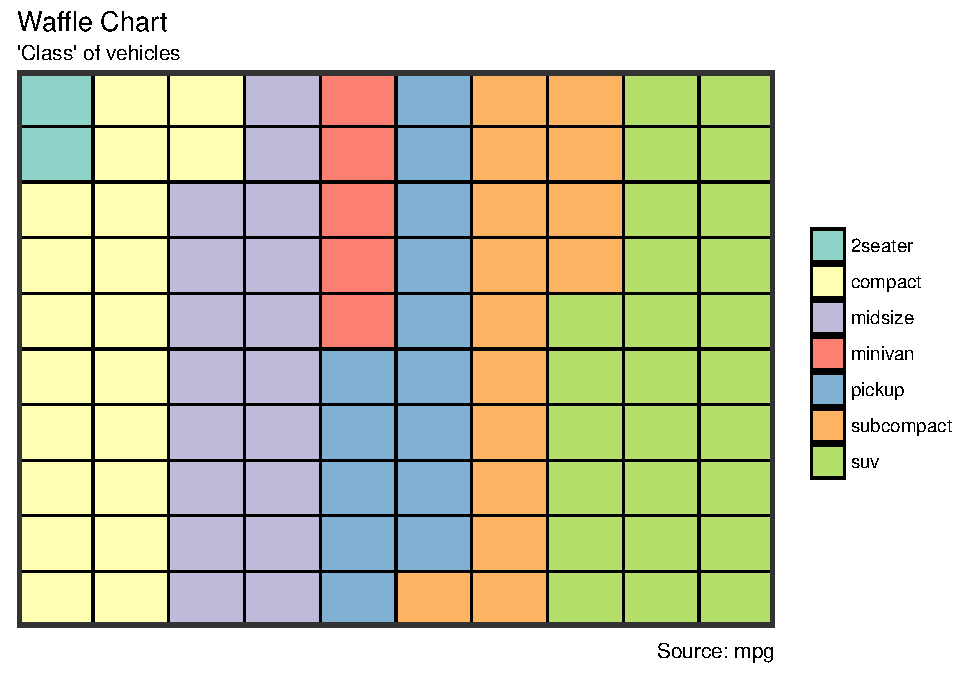
\includegraphics{ggplot2-50examples_files/figure-latex/unnamed-chunk-30-1.pdf}
\newpage

\textbf{Pie Chart}

Pie chart, a classic way of showing the compositions is equivalent to
the waffle chart in terms of the information conveyed. But is a slightly
tricky to implement in ggplot2 using the coord\_polar().

\begin{Shaded}
\begin{Highlighting}[]
\KeywordTok{library}\NormalTok{(ggplot2)}
\KeywordTok{theme_set}\NormalTok{(}\KeywordTok{theme_classic}\NormalTok{())}

\CommentTok{# Source: Frequency table}
\NormalTok{df <-}\StringTok{ }\KeywordTok{as.data.frame}\NormalTok{(}\KeywordTok{table}\NormalTok{(mpg}\OperatorTok{$}\NormalTok{class))}
\KeywordTok{colnames}\NormalTok{(df) <-}\StringTok{ }\KeywordTok{c}\NormalTok{(}\StringTok{"class"}\NormalTok{, }\StringTok{"freq"}\NormalTok{)}
\NormalTok{pie <-}\StringTok{ }\KeywordTok{ggplot}\NormalTok{(df, }\KeywordTok{aes}\NormalTok{(}\DataTypeTok{x =} \StringTok{""}\NormalTok{, }\DataTypeTok{y=}\NormalTok{freq, }\DataTypeTok{fill =} \KeywordTok{factor}\NormalTok{(class))) }\OperatorTok{+}\StringTok{ }
\StringTok{  }\KeywordTok{geom_bar}\NormalTok{(}\DataTypeTok{width =} \DecValTok{1}\NormalTok{, }\DataTypeTok{stat =} \StringTok{"identity"}\NormalTok{) }\OperatorTok{+}
\StringTok{  }\KeywordTok{theme}\NormalTok{(}\DataTypeTok{axis.line =} \KeywordTok{element_blank}\NormalTok{(), }
        \DataTypeTok{plot.title =} \KeywordTok{element_text}\NormalTok{(}\DataTypeTok{hjust=}\FloatTok{0.5}\NormalTok{)) }\OperatorTok{+}\StringTok{ }
\StringTok{  }\KeywordTok{labs}\NormalTok{(}\DataTypeTok{fill=}\StringTok{"class"}\NormalTok{, }
       \DataTypeTok{x=}\OtherTok{NULL}\NormalTok{, }
       \DataTypeTok{y=}\OtherTok{NULL}\NormalTok{, }
       \DataTypeTok{title=}\StringTok{"Pie Chart of class"}\NormalTok{, }
       \DataTypeTok{caption=}\StringTok{"Source: mpg"}\NormalTok{)}

\NormalTok{pie }\OperatorTok{+}\StringTok{ }\KeywordTok{coord_polar}\NormalTok{(}\DataTypeTok{theta =} \StringTok{"y"}\NormalTok{, }\DataTypeTok{start=}\DecValTok{0}\NormalTok{)}
\end{Highlighting}
\end{Shaded}

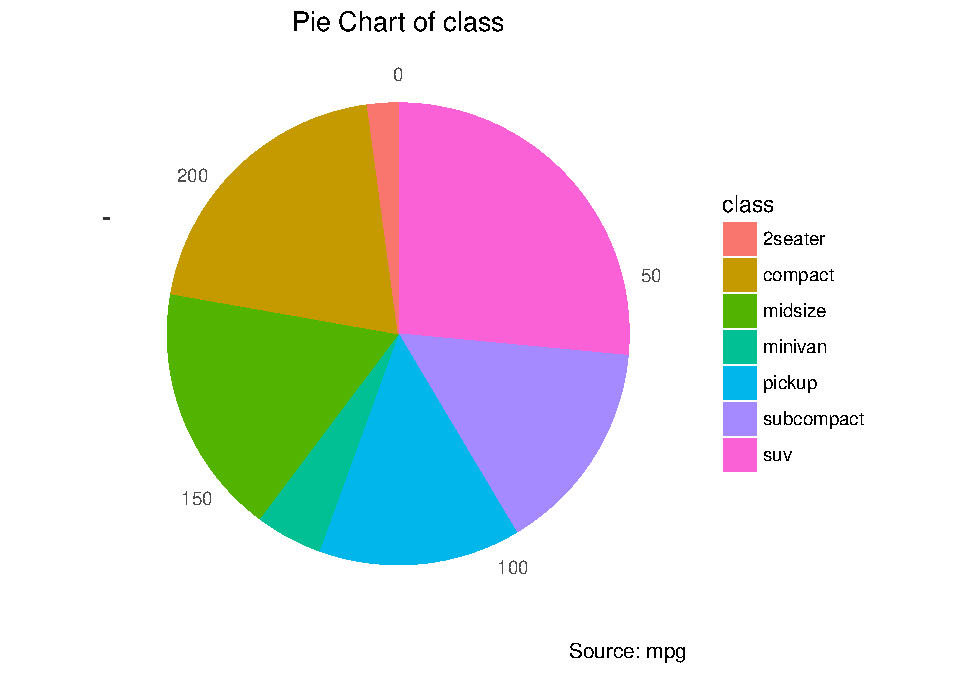
\includegraphics{ggplot2-50examples_files/figure-latex/unnamed-chunk-31-1.pdf}

\begin{Shaded}
\begin{Highlighting}[]
\CommentTok{# Source: Categorical variable.}
\CommentTok{# mpg$class}
\NormalTok{pie <-}\StringTok{ }\KeywordTok{ggplot}\NormalTok{(mpg, }\KeywordTok{aes}\NormalTok{(}\DataTypeTok{x =} \StringTok{""}\NormalTok{, }\DataTypeTok{fill =} \KeywordTok{factor}\NormalTok{(class))) }\OperatorTok{+}\StringTok{ }
\StringTok{  }\KeywordTok{geom_bar}\NormalTok{(}\DataTypeTok{width =} \DecValTok{1}\NormalTok{) }\OperatorTok{+}
\StringTok{  }\KeywordTok{theme}\NormalTok{(}\DataTypeTok{axis.line =} \KeywordTok{element_blank}\NormalTok{(), }
        \DataTypeTok{plot.title =} \KeywordTok{element_text}\NormalTok{(}\DataTypeTok{hjust=}\FloatTok{0.5}\NormalTok{)) }\OperatorTok{+}\StringTok{ }
\StringTok{  }\KeywordTok{labs}\NormalTok{(}\DataTypeTok{fill=}\StringTok{"class"}\NormalTok{, }
       \DataTypeTok{x=}\OtherTok{NULL}\NormalTok{, }
       \DataTypeTok{y=}\OtherTok{NULL}\NormalTok{, }
       \DataTypeTok{title=}\StringTok{"Pie Chart of class"}\NormalTok{, }
       \DataTypeTok{caption=}\StringTok{"Source: mpg"}\NormalTok{)}
  
\NormalTok{pie }\OperatorTok{+}\StringTok{ }\KeywordTok{coord_polar}\NormalTok{(}\DataTypeTok{theta =} \StringTok{"y"}\NormalTok{, }\DataTypeTok{start=}\DecValTok{0}\NormalTok{)}
\end{Highlighting}
\end{Shaded}

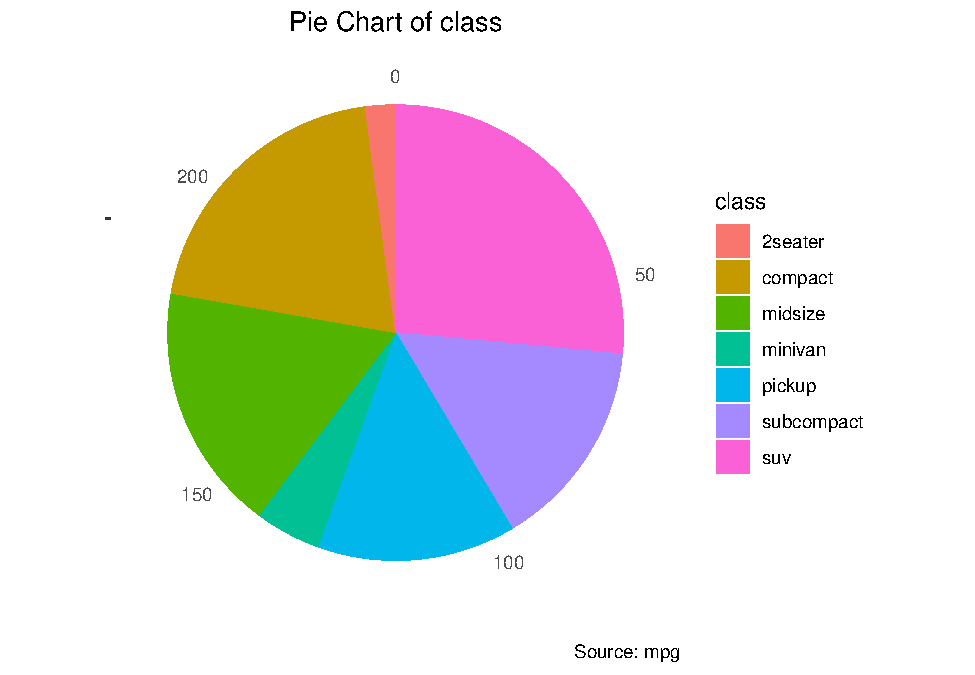
\includegraphics{ggplot2-50examples_files/figure-latex/unnamed-chunk-31-2.pdf}

\begin{Shaded}
\begin{Highlighting}[]
\CommentTok{# http://www.r-graph-gallery.com/128-ring-or-donut-plot/}
\end{Highlighting}
\end{Shaded}

\newpage

\textbf{Bar Chart}

By default, \texttt{geom\_bar()} has the stat set to count. That means,
when you provide just a continuous X variable (and no Y variable), it
tries to make a histogram out of the data.

In order to make a bar chart create bars instead of histogram, you need
to do two things.

\begin{quote}
Set stat=identity Provide both x and y inside \texttt{aes()} where, x is
either character or factor and y is numeric.
\end{quote}

A bar chart can be drawn from a categorical column variable or from a
separate frequency table. By adjusting width, you can adjust the
thickness of the bars. If your data source is a frequency table, that
is, if you don't want ggplot to compute the counts, you need to set the
stat=identity inside the \texttt{geom\_bar()}.

\begin{Shaded}
\begin{Highlighting}[]
\CommentTok{# prep frequency table}
\NormalTok{freqtable <-}\StringTok{ }\KeywordTok{table}\NormalTok{(mpg}\OperatorTok{$}\NormalTok{manufacturer)}
\NormalTok{df <-}\StringTok{ }\KeywordTok{as.data.frame.table}\NormalTok{(freqtable)}
\KeywordTok{head}\NormalTok{(df)}
\end{Highlighting}
\end{Shaded}

\begin{verbatim}
##        Var1 Freq
## 1      audi   18
## 2 chevrolet   19
## 3     dodge   37
## 4      ford   25
## 5     honda    9
## 6   hyundai   14
\end{verbatim}

\begin{Shaded}
\begin{Highlighting}[]
\CommentTok{# plot}
\KeywordTok{library}\NormalTok{(ggplot2)}
\KeywordTok{theme_set}\NormalTok{(}\KeywordTok{theme_classic}\NormalTok{())}

\CommentTok{# Plot}
\NormalTok{g <-}\StringTok{ }\KeywordTok{ggplot}\NormalTok{(df, }\KeywordTok{aes}\NormalTok{(Var1, Freq))}
\NormalTok{g }\OperatorTok{+}\StringTok{ }\KeywordTok{geom_bar}\NormalTok{(}\DataTypeTok{stat=}\StringTok{"identity"}\NormalTok{, }\DataTypeTok{width =} \FloatTok{0.5}\NormalTok{, }\DataTypeTok{fill=}\StringTok{"tomato2"}\NormalTok{) }\OperatorTok{+}\StringTok{ }
\StringTok{      }\KeywordTok{labs}\NormalTok{(}\DataTypeTok{title=}\StringTok{"Bar Chart"}\NormalTok{, }
           \DataTypeTok{subtitle=}\StringTok{"Manufacturer of vehicles"}\NormalTok{, }
           \DataTypeTok{caption=}\StringTok{"Source: Frequency of Manufacturers from 'mpg' dataset"}\NormalTok{) }\OperatorTok{+}
\StringTok{      }\KeywordTok{theme}\NormalTok{(}\DataTypeTok{axis.text.x =} \KeywordTok{element_text}\NormalTok{(}\DataTypeTok{angle=}\DecValTok{65}\NormalTok{, }\DataTypeTok{vjust=}\FloatTok{0.6}\NormalTok{))}
\end{Highlighting}
\end{Shaded}

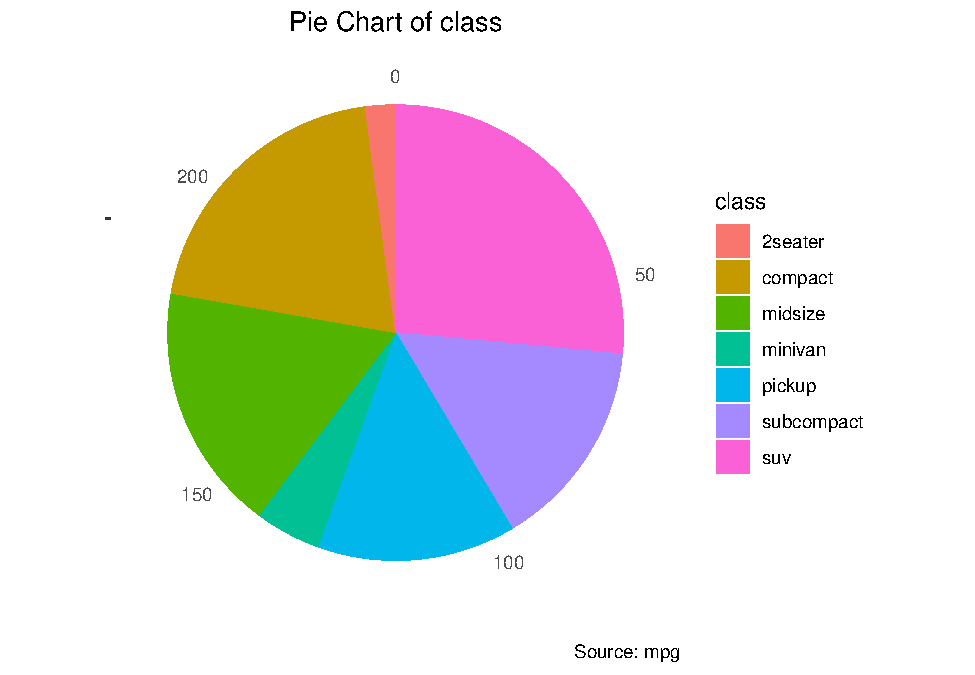
\includegraphics{ggplot2-50examples_files/figure-latex/unnamed-chunk-34-1.pdf}

It can be computed directly from a column variable as well. In this
case, only X is provided and \texttt{stat=identity} is not set.

\begin{Shaded}
\begin{Highlighting}[]
\CommentTok{# From on a categorical column variable}
\NormalTok{g <-}\StringTok{ }\KeywordTok{ggplot}\NormalTok{(mpg, }\KeywordTok{aes}\NormalTok{(manufacturer))}
\NormalTok{g }\OperatorTok{+}\StringTok{ }\KeywordTok{geom_bar}\NormalTok{(}\KeywordTok{aes}\NormalTok{(}\DataTypeTok{fill=}\NormalTok{class), }\DataTypeTok{width =} \FloatTok{0.5}\NormalTok{) }\OperatorTok{+}\StringTok{ }
\StringTok{  }\KeywordTok{theme}\NormalTok{(}\DataTypeTok{axis.text.x =} \KeywordTok{element_text}\NormalTok{(}\DataTypeTok{angle=}\DecValTok{65}\NormalTok{, }\DataTypeTok{vjust=}\FloatTok{0.6}\NormalTok{)) }\OperatorTok{+}
\StringTok{  }\KeywordTok{labs}\NormalTok{(}\DataTypeTok{title=}\StringTok{"Categorywise Bar Chart"}\NormalTok{, }
       \DataTypeTok{subtitle=}\StringTok{"Manufacturer of vehicles"}\NormalTok{, }
       \DataTypeTok{caption=}\StringTok{"Source: Manufacturers from 'mpg' dataset"}\NormalTok{)}
\end{Highlighting}
\end{Shaded}

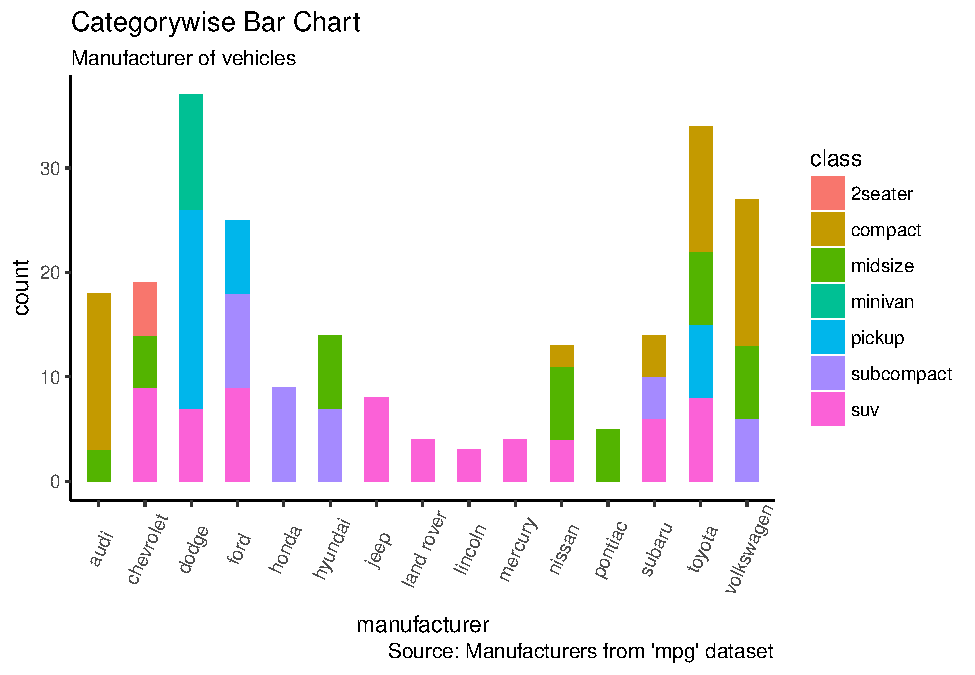
\includegraphics{ggplot2-50examples_files/figure-latex/unnamed-chunk-35-1.pdf}

\newpage

blank

\newpage

\subsection{6. Change}\label{change}

\textbf{Time Series Plot From a Time Series Object (ts)}

The ggfortify package allows autoplot to automatically plot directly
from a time series object (ts).

\begin{Shaded}
\begin{Highlighting}[]
\NormalTok{## From Timeseries object (ts)}
\KeywordTok{library}\NormalTok{(ggplot2)}
\KeywordTok{library}\NormalTok{(ggfortify)}
\KeywordTok{theme_set}\NormalTok{(}\KeywordTok{theme_classic}\NormalTok{())}

\CommentTok{# Plot }
\KeywordTok{autoplot}\NormalTok{(AirPassengers) }\OperatorTok{+}\StringTok{ }
\StringTok{  }\KeywordTok{labs}\NormalTok{(}\DataTypeTok{title=}\StringTok{"AirPassengers"}\NormalTok{) }\OperatorTok{+}\StringTok{ }
\StringTok{  }\KeywordTok{theme}\NormalTok{(}\DataTypeTok{plot.title =} \KeywordTok{element_text}\NormalTok{(}\DataTypeTok{hjust=}\FloatTok{0.5}\NormalTok{))}
\end{Highlighting}
\end{Shaded}

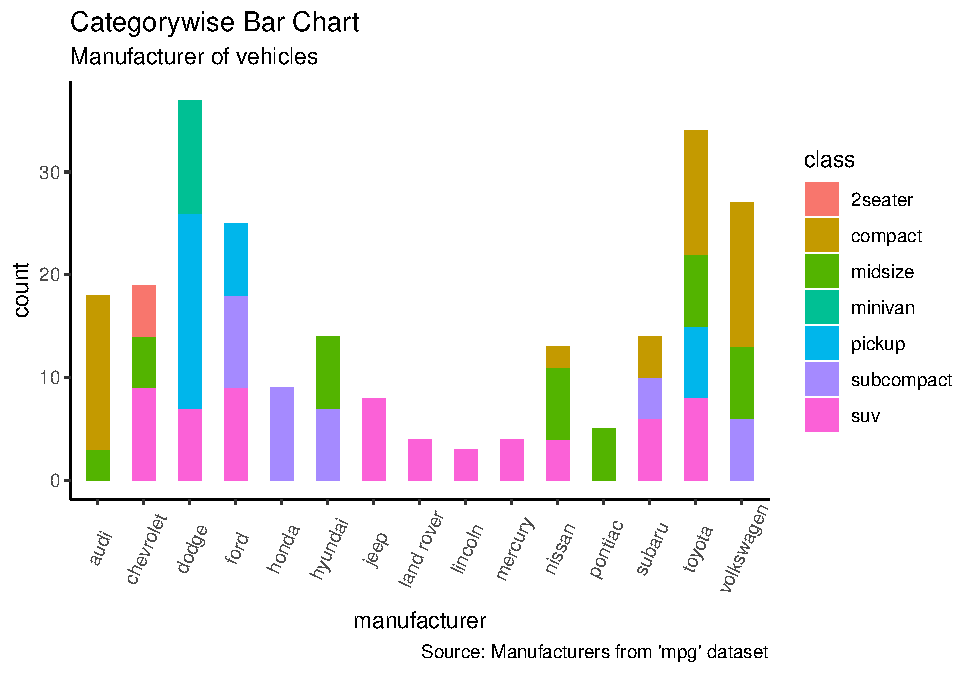
\includegraphics{ggplot2-50examples_files/figure-latex/unnamed-chunk-36-1.pdf}

\newpage

\textbf{Time Series Plot From a Data Frame}

Using \texttt{geom\_line()}, a time series (or line chart) can be drawn
from a data.frame as well. The X axis breaks are generated by default.
In below example, the breaks are formed once every 10 years.

\emph{Default X Axis Labels}

\begin{Shaded}
\begin{Highlighting}[]
\KeywordTok{library}\NormalTok{(ggplot2)}
\KeywordTok{theme_set}\NormalTok{(}\KeywordTok{theme_classic}\NormalTok{())}

\CommentTok{# Allow Default X Axis Labels}
\KeywordTok{ggplot}\NormalTok{(economics, }\KeywordTok{aes}\NormalTok{(}\DataTypeTok{x=}\NormalTok{date)) }\OperatorTok{+}\StringTok{ }
\StringTok{  }\KeywordTok{geom_line}\NormalTok{(}\KeywordTok{aes}\NormalTok{(}\DataTypeTok{y=}\NormalTok{returns_perc)) }\OperatorTok{+}\StringTok{ }
\StringTok{  }\KeywordTok{labs}\NormalTok{(}\DataTypeTok{title=}\StringTok{"Time Series Chart"}\NormalTok{, }
       \DataTypeTok{subtitle=}\StringTok{"Returns Percentage from 'Economics' Dataset"}\NormalTok{, }
       \DataTypeTok{caption=}\StringTok{"Source: Economics"}\NormalTok{, }
       \DataTypeTok{y=}\StringTok{"Returns %"}\NormalTok{)}
\end{Highlighting}
\end{Shaded}

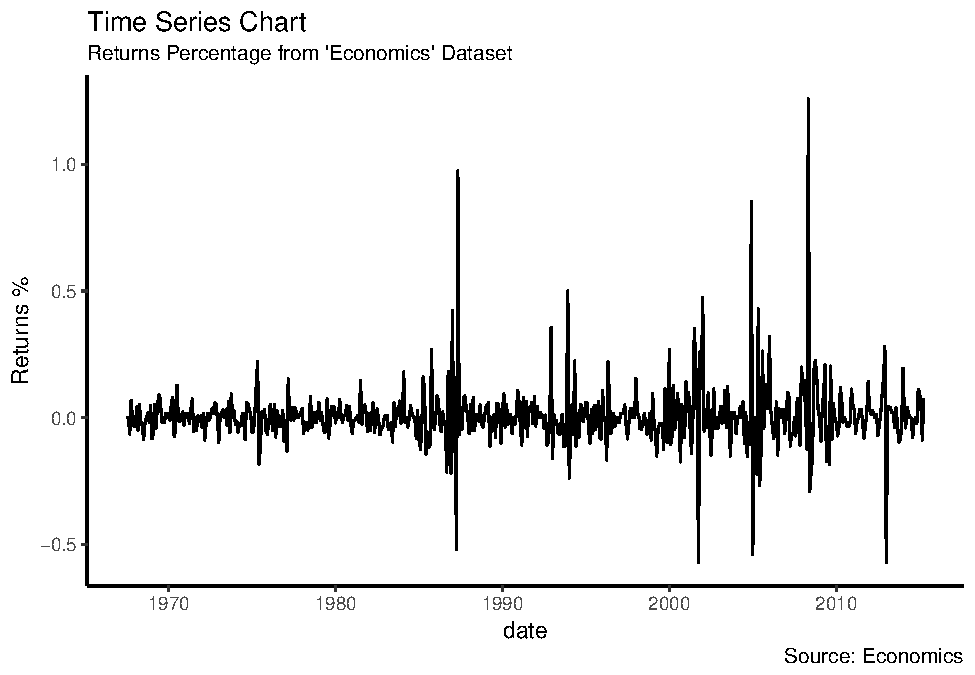
\includegraphics{ggplot2-50examples_files/figure-latex/unnamed-chunk-37-1.pdf}

\newpage

\textbf{Time Series Plot For a Monthly Time Series}

If you want to set your own time intervals (breaks) in X axis, you need
to set the breaks and labels using \texttt{scale\_x\_date()}.

\begin{Shaded}
\begin{Highlighting}[]
\KeywordTok{library}\NormalTok{(ggplot2)}
\KeywordTok{library}\NormalTok{(lubridate)}
\end{Highlighting}
\end{Shaded}

\begin{verbatim}
## 
## Attaching package: 'lubridate'
\end{verbatim}

\begin{verbatim}
## The following object is masked from 'package:base':
## 
##     date
\end{verbatim}

\begin{Shaded}
\begin{Highlighting}[]
\KeywordTok{theme_set}\NormalTok{(}\KeywordTok{theme_bw}\NormalTok{())}

\NormalTok{economics_m <-}\StringTok{ }\NormalTok{economics[}\DecValTok{1}\OperatorTok{:}\DecValTok{24}\NormalTok{, ]}

\CommentTok{# labels and breaks for X axis text}
\NormalTok{lbls <-}\StringTok{ }\KeywordTok{paste0}\NormalTok{(month.abb[}\KeywordTok{month}\NormalTok{(economics_m}\OperatorTok{$}\NormalTok{date)], }\StringTok{" "}\NormalTok{, lubridate}\OperatorTok{::}\KeywordTok{year}\NormalTok{(economics_m}\OperatorTok{$}\NormalTok{date))}
\NormalTok{brks <-}\StringTok{ }\NormalTok{economics_m}\OperatorTok{$}\NormalTok{date}

\CommentTok{# plot}
\KeywordTok{ggplot}\NormalTok{(economics_m, }\KeywordTok{aes}\NormalTok{(}\DataTypeTok{x=}\NormalTok{date)) }\OperatorTok{+}\StringTok{ }
\StringTok{  }\KeywordTok{geom_line}\NormalTok{(}\KeywordTok{aes}\NormalTok{(}\DataTypeTok{y=}\NormalTok{returns_perc)) }\OperatorTok{+}\StringTok{ }
\StringTok{  }\KeywordTok{labs}\NormalTok{(}\DataTypeTok{title=}\StringTok{"Monthly Time Series"}\NormalTok{, }
       \DataTypeTok{subtitle=}\StringTok{"Returns Percentage from Economics Dataset"}\NormalTok{, }
       \DataTypeTok{caption=}\StringTok{"Source: Economics"}\NormalTok{, }
       \DataTypeTok{y=}\StringTok{"Returns %"}\NormalTok{) }\OperatorTok{+}\StringTok{  }\CommentTok{# title and caption}
\StringTok{  }\KeywordTok{scale_x_date}\NormalTok{(}\DataTypeTok{labels =}\NormalTok{ lbls, }
               \DataTypeTok{breaks =}\NormalTok{ brks) }\OperatorTok{+}\StringTok{  }\CommentTok{# change to monthly ticks and labels}
\StringTok{  }\KeywordTok{theme}\NormalTok{(}\DataTypeTok{axis.text.x =} \KeywordTok{element_text}\NormalTok{(}\DataTypeTok{angle =} \DecValTok{90}\NormalTok{, }\DataTypeTok{vjust=}\FloatTok{0.5}\NormalTok{),  }\CommentTok{# rotate x axis text}
        \DataTypeTok{panel.grid.minor =} \KeywordTok{element_blank}\NormalTok{())  }\CommentTok{# turn off minor grid}
\end{Highlighting}
\end{Shaded}

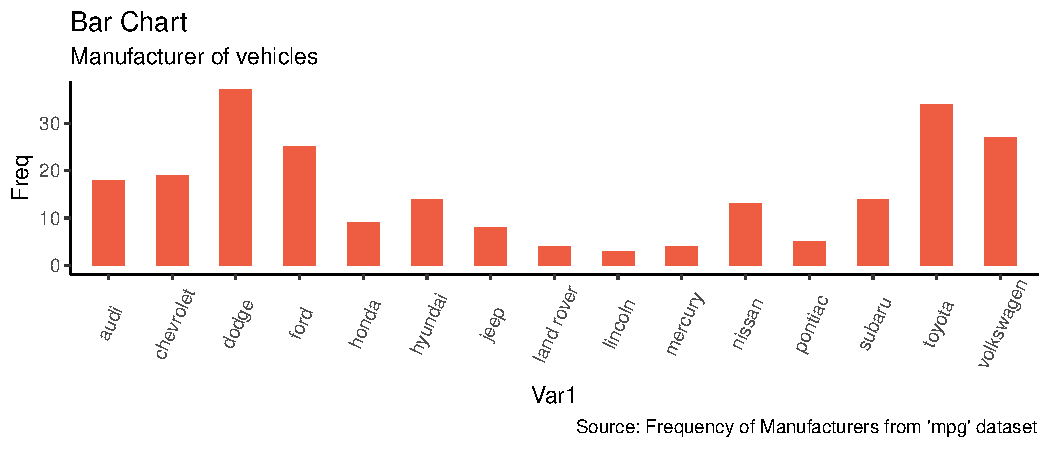
\includegraphics{ggplot2-50examples_files/figure-latex/unnamed-chunk-38-1.pdf}
\newpage

\textbf{Time Series Plot For a Yearly Time Series}

\begin{Shaded}
\begin{Highlighting}[]
\KeywordTok{library}\NormalTok{(ggplot2)}
\KeywordTok{library}\NormalTok{(lubridate)}
\KeywordTok{theme_set}\NormalTok{(}\KeywordTok{theme_bw}\NormalTok{())}

\NormalTok{economics_y <-}\StringTok{ }\NormalTok{economics[}\DecValTok{1}\OperatorTok{:}\DecValTok{90}\NormalTok{, ]}

\CommentTok{# labels and breaks for X axis text}
\NormalTok{brks <-}\StringTok{ }\NormalTok{economics_y}\OperatorTok{$}\NormalTok{date[}\KeywordTok{seq}\NormalTok{(}\DecValTok{1}\NormalTok{, }\KeywordTok{length}\NormalTok{(economics_y}\OperatorTok{$}\NormalTok{date), }\DecValTok{12}\NormalTok{)]}
\NormalTok{lbls <-}\StringTok{ }\NormalTok{lubridate}\OperatorTok{::}\KeywordTok{year}\NormalTok{(brks)}

\CommentTok{# plot}
\KeywordTok{ggplot}\NormalTok{(economics_y, }\KeywordTok{aes}\NormalTok{(}\DataTypeTok{x=}\NormalTok{date)) }\OperatorTok{+}\StringTok{ }
\StringTok{  }\KeywordTok{geom_line}\NormalTok{(}\KeywordTok{aes}\NormalTok{(}\DataTypeTok{y=}\NormalTok{returns_perc)) }\OperatorTok{+}\StringTok{ }
\StringTok{  }\KeywordTok{labs}\NormalTok{(}\DataTypeTok{title=}\StringTok{"Yearly Time Series"}\NormalTok{, }
       \DataTypeTok{subtitle=}\StringTok{"Returns Percentage from Economics Dataset"}\NormalTok{, }
       \DataTypeTok{caption=}\StringTok{"Source: Economics"}\NormalTok{, }
       \DataTypeTok{y=}\StringTok{"Returns %"}\NormalTok{) }\OperatorTok{+}\StringTok{  }\CommentTok{# title and caption}
\StringTok{  }\KeywordTok{scale_x_date}\NormalTok{(}\DataTypeTok{labels =}\NormalTok{ lbls, }
               \DataTypeTok{breaks =}\NormalTok{ brks) }\OperatorTok{+}\StringTok{  }\CommentTok{# change to monthly ticks and labels}
\StringTok{  }\KeywordTok{theme}\NormalTok{(}\DataTypeTok{axis.text.x =} \KeywordTok{element_text}\NormalTok{(}\DataTypeTok{angle =} \DecValTok{90}\NormalTok{, }\DataTypeTok{vjust=}\FloatTok{0.5}\NormalTok{),  }\CommentTok{# rotate x axis text}
        \DataTypeTok{panel.grid.minor =} \KeywordTok{element_blank}\NormalTok{())  }\CommentTok{# turn off minor grid}
\end{Highlighting}
\end{Shaded}

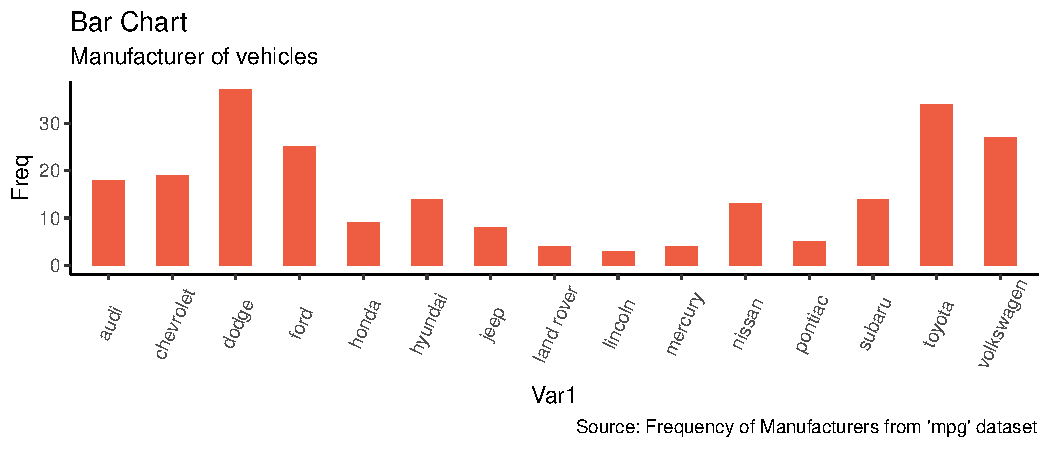
\includegraphics{ggplot2-50examples_files/figure-latex/unnamed-chunk-39-1.pdf}

\newpage

blank

\newpage

\textbf{Time Series Plot From Long Data Format: Multiple Time Series in
Same Dataframe Column}

In this example, I construct the ggplot from a long data format. That
means, the column names and respective values of all the columns are
stacked in just 2 variables (variable and value respectively). If you
were to convert this data to wide format, it would look like the
economics dataset.

In below example, the geom\_line is drawn for value column and the
aes(col) is set to variable. This way, with just one call to geom\_line,
multiple colored lines are drawn, one each for each unique value in
variable column. The \texttt{scale\_x\_date()} changes the X axis breaks
and labels, and scale\_color\_manual changes the color of the lines.

\begin{Shaded}
\begin{Highlighting}[]
\KeywordTok{data}\NormalTok{(economics_long, }\DataTypeTok{package =} \StringTok{"ggplot2"}\NormalTok{)}
\KeywordTok{head}\NormalTok{(economics_long)}
\end{Highlighting}
\end{Shaded}

\begin{verbatim}
## # A tibble: 6 x 4
## # Groups:   variable [1]
##   date       variable value  value01
##   <date>     <fct>    <dbl>    <dbl>
## 1 1967-07-01 pce       507. 0       
## 2 1967-08-01 pce       510. 0.000266
## 3 1967-09-01 pce       516. 0.000764
## 4 1967-10-01 pce       513. 0.000472
## 5 1967-11-01 pce       518. 0.000918
## 6 1967-12-01 pce       526. 0.00158
\end{verbatim}

\begin{Shaded}
\begin{Highlighting}[]
\KeywordTok{library}\NormalTok{(ggplot2)}
\KeywordTok{library}\NormalTok{(lubridate)}
\KeywordTok{theme_set}\NormalTok{(}\KeywordTok{theme_bw}\NormalTok{())}

\NormalTok{df <-}\StringTok{ }\NormalTok{economics_long[economics_long}\OperatorTok{$}\NormalTok{variable }\OperatorTok\StringTok{ }\KeywordTok{c}\NormalTok{(}\StringTok{"psavert"}\NormalTok{, }\StringTok{"uempmed"}\NormalTok{), ]}
\NormalTok{df <-}\StringTok{ }\NormalTok{df[lubridate}\OperatorTok{::}\KeywordTok{year}\NormalTok{(df}\OperatorTok{$}\NormalTok{date) }\OperatorTok\StringTok{ }\KeywordTok{c}\NormalTok{(}\DecValTok{1967}\OperatorTok{:}\DecValTok{1981}\NormalTok{), ]}

\CommentTok{# labels and breaks for X axis text}
\NormalTok{brks <-}\StringTok{ }\NormalTok{df}\OperatorTok{$}\NormalTok{date[}\KeywordTok{seq}\NormalTok{(}\DecValTok{1}\NormalTok{, }\KeywordTok{length}\NormalTok{(df}\OperatorTok{$}\NormalTok{date), }\DecValTok{12}\NormalTok{)]}
\NormalTok{lbls <-}\StringTok{ }\NormalTok{lubridate}\OperatorTok{::}\KeywordTok{year}\NormalTok{(brks)}

\CommentTok{# plot}
\KeywordTok{ggplot}\NormalTok{(df, }\KeywordTok{aes}\NormalTok{(}\DataTypeTok{x=}\NormalTok{date)) }\OperatorTok{+}\StringTok{ }
\StringTok{  }\KeywordTok{geom_line}\NormalTok{(}\KeywordTok{aes}\NormalTok{(}\DataTypeTok{y=}\NormalTok{value, }\DataTypeTok{col=}\NormalTok{variable)) }\OperatorTok{+}\StringTok{ }
\StringTok{  }\KeywordTok{labs}\NormalTok{(}\DataTypeTok{title=}\StringTok{"Time Series of Returns Percentage"}\NormalTok{, }
       \DataTypeTok{subtitle=}\StringTok{"Drawn from Long Data format"}\NormalTok{, }
       \DataTypeTok{caption=}\StringTok{"Source: Economics"}\NormalTok{, }
       \DataTypeTok{y=}\StringTok{"Returns %"}\NormalTok{, }
       \DataTypeTok{color=}\OtherTok{NULL}\NormalTok{) }\OperatorTok{+}\StringTok{  }\CommentTok{# title and caption}
\StringTok{  }\KeywordTok{scale_x_date}\NormalTok{(}\DataTypeTok{labels =}\NormalTok{ lbls, }\DataTypeTok{breaks =}\NormalTok{ brks) }\OperatorTok{+}\StringTok{  }\CommentTok{# change to monthly ticks and labels}
\StringTok{  }\KeywordTok{scale_color_manual}\NormalTok{(}\DataTypeTok{labels =} \KeywordTok{c}\NormalTok{(}\StringTok{"psavert"}\NormalTok{, }\StringTok{"uempmed"}\NormalTok{), }
                     \DataTypeTok{values =} \KeywordTok{c}\NormalTok{(}\StringTok{"psavert"}\NormalTok{=}\StringTok{"#00ba38"}\NormalTok{, }\StringTok{"uempmed"}\NormalTok{=}\StringTok{"#f8766d"}\NormalTok{)) }\OperatorTok{+}\StringTok{  }\CommentTok{# line color}
\StringTok{  }\KeywordTok{theme}\NormalTok{(}\DataTypeTok{axis.text.x =} \KeywordTok{element_text}\NormalTok{(}\DataTypeTok{angle =} \DecValTok{90}\NormalTok{, }\DataTypeTok{vjust=}\FloatTok{0.5}\NormalTok{, }\DataTypeTok{size =} \DecValTok{8}\NormalTok{),  }\CommentTok{# rotate x axis text}
        \DataTypeTok{panel.grid.minor =} \KeywordTok{element_blank}\NormalTok{())  }\CommentTok{# turn off minor grid}
\end{Highlighting}
\end{Shaded}

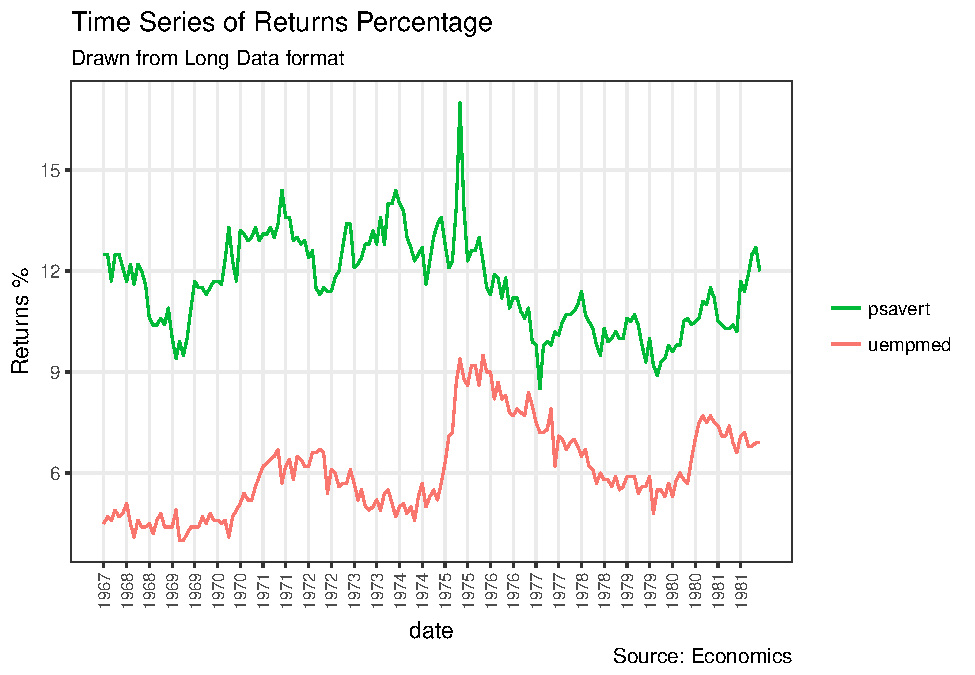
\includegraphics{ggplot2-50examples_files/figure-latex/unnamed-chunk-40-1.pdf}
\newpage

\textbf{Time Series Plot From Wide Data Format: Data in Multiple Columns
of Dataframe}

As noted in the part 2 of this tutorial, whenever your plot's geom (like
points, lines, bars, etc) changes the fill, size, col, shape or stroke
based on another column, a legend is automatically drawn.

But if you are creating a time series (or even other types of plots)
from a wide data format, you have to draw each line manually by calling
\texttt{geom\_line()} once for every line. So, a legend will not be
drawn by default.

However, having a legend would still be nice. This can be done using the
\texttt{scale\_aesthetic\_manual()} format of functions (like,
\texttt{scale\_color\_manual()} if only the color of your lines change).
Using this function, you can give a legend title with the name argument,
tell what color the legend should take with the values argument and also
set the legend labels.

Even though the below plot looks exactly like the previous one, the
approach to construct this is different.

You might wonder why I used this function in previous example for long
data format as well. Note that, in previous example, it was used to
change the color of the line only. Without scale\_color\_manual(), you
would still have got a legend, but the lines would be of a different
(default) color. But in current example, without scale\_color\_manual(),
you wouldn't even have a legend. Try it out!

\begin{Shaded}
\begin{Highlighting}[]
\KeywordTok{library}\NormalTok{(ggplot2)}
\KeywordTok{library}\NormalTok{(lubridate)}
\KeywordTok{theme_set}\NormalTok{(}\KeywordTok{theme_bw}\NormalTok{())}

\NormalTok{df <-}\StringTok{ }\NormalTok{economics[, }\KeywordTok{c}\NormalTok{(}\StringTok{"date"}\NormalTok{, }\StringTok{"psavert"}\NormalTok{, }\StringTok{"uempmed"}\NormalTok{)]}
\NormalTok{df <-}\StringTok{ }\NormalTok{df[lubridate}\OperatorTok{::}\KeywordTok{year}\NormalTok{(df}\OperatorTok{$}\NormalTok{date) }\OperatorTok\StringTok{ }\KeywordTok{c}\NormalTok{(}\DecValTok{1967}\OperatorTok{:}\DecValTok{1981}\NormalTok{), ]}

\CommentTok{# labels and breaks for X axis text}
\NormalTok{brks <-}\StringTok{ }\NormalTok{df}\OperatorTok{$}\NormalTok{date[}\KeywordTok{seq}\NormalTok{(}\DecValTok{1}\NormalTok{, }\KeywordTok{length}\NormalTok{(df}\OperatorTok{$}\NormalTok{date), }\DecValTok{12}\NormalTok{)]}
\NormalTok{lbls <-}\StringTok{ }\NormalTok{lubridate}\OperatorTok{::}\KeywordTok{year}\NormalTok{(brks)}

\CommentTok{# plot}
\KeywordTok{ggplot}\NormalTok{(df, }\KeywordTok{aes}\NormalTok{(}\DataTypeTok{x=}\NormalTok{date)) }\OperatorTok{+}\StringTok{ }
\StringTok{  }\KeywordTok{geom_line}\NormalTok{(}\KeywordTok{aes}\NormalTok{(}\DataTypeTok{y=}\NormalTok{psavert, }\DataTypeTok{col=}\StringTok{"psavert"}\NormalTok{)) }\OperatorTok{+}\StringTok{ }
\StringTok{  }\KeywordTok{geom_line}\NormalTok{(}\KeywordTok{aes}\NormalTok{(}\DataTypeTok{y=}\NormalTok{uempmed, }\DataTypeTok{col=}\StringTok{"uempmed"}\NormalTok{)) }\OperatorTok{+}\StringTok{ }
\StringTok{  }\KeywordTok{labs}\NormalTok{(}\DataTypeTok{title=}\StringTok{"Time Series of Returns Percentage"}\NormalTok{, }
       \DataTypeTok{subtitle=}\StringTok{"Drawn From Wide Data format"}\NormalTok{, }
       \DataTypeTok{caption=}\StringTok{"Source: Economics"}\NormalTok{, }\DataTypeTok{y=}\StringTok{"Returns %"}\NormalTok{) }\OperatorTok{+}\StringTok{  }\CommentTok{# title and caption}
\StringTok{  }\KeywordTok{scale_x_date}\NormalTok{(}\DataTypeTok{labels =}\NormalTok{ lbls, }\DataTypeTok{breaks =}\NormalTok{ brks) }\OperatorTok{+}\StringTok{  }\CommentTok{# change to monthly ticks and labels}
\StringTok{  }\KeywordTok{scale_color_manual}\NormalTok{(}\DataTypeTok{name=}\StringTok{""}\NormalTok{, }
                     \DataTypeTok{values =} \KeywordTok{c}\NormalTok{(}\StringTok{"psavert"}\NormalTok{=}\StringTok{"#00ba38"}\NormalTok{, }\StringTok{"uempmed"}\NormalTok{=}\StringTok{"#f8766d"}\NormalTok{)) }\OperatorTok{+}\StringTok{  }\CommentTok{# line color}
\StringTok{  }\KeywordTok{theme}\NormalTok{(}\DataTypeTok{panel.grid.minor =} \KeywordTok{element_blank}\NormalTok{())  }\CommentTok{# turn off minor grid}
\end{Highlighting}
\end{Shaded}

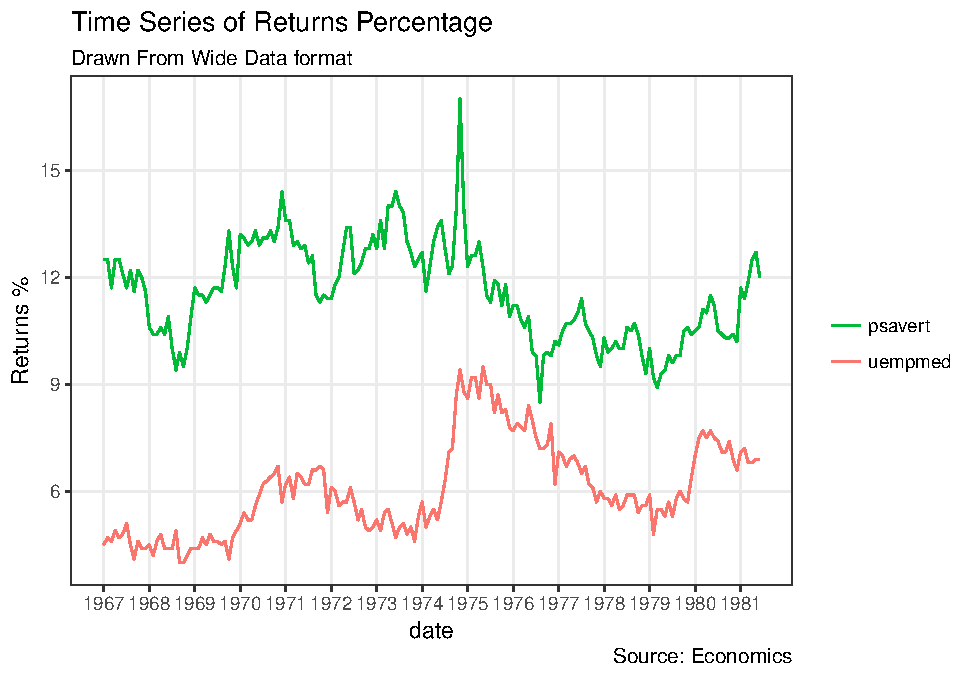
\includegraphics{ggplot2-50examples_files/figure-latex/unnamed-chunk-41-1.pdf}
\newpage

\textbf{Stacked Area Chart}

Stacked area chart is just like a line chart, except that the region
below the plot is all colored. This is typically used when:

\begin{quote}
You want to describe how a quantity or volume (rather than something
like price) changed over time You have many data points. For very few
data points, consider plotting a bar chart. You want to show the
contribution from individual components. This can be plotted using
geom\_area which works very much like geom\_line. But there is an
important point to note. By default, each \texttt{geom\_area()} starts
from the bottom of Y axis (which is typically 0), but, if you want to
show the contribution from individual components, you want the
geom\_area to be stacked over the top of previous component, rather than
the floor of the plot itself. So, you have to add all the bottom layers
while setting the y of geom\_area.
\end{quote}

In below example, I have set it as y=psavert+uempmed for the topmost
\texttt{geom\_area()}.

However nice the plot looks, the caveat is that, it can easily become
complicated and uninterprettable if there are too many components.

\begin{Shaded}
\begin{Highlighting}[]
\KeywordTok{library}\NormalTok{(ggplot2)}
\KeywordTok{library}\NormalTok{(lubridate)}
\KeywordTok{theme_set}\NormalTok{(}\KeywordTok{theme_bw}\NormalTok{())}

\NormalTok{df <-}\StringTok{ }\NormalTok{economics[, }\KeywordTok{c}\NormalTok{(}\StringTok{"date"}\NormalTok{, }\StringTok{"psavert"}\NormalTok{, }\StringTok{"uempmed"}\NormalTok{)]}
\NormalTok{df <-}\StringTok{ }\NormalTok{df[lubridate}\OperatorTok{::}\KeywordTok{year}\NormalTok{(df}\OperatorTok{$}\NormalTok{date) }\OperatorTok\StringTok{ }\KeywordTok{c}\NormalTok{(}\DecValTok{1967}\OperatorTok{:}\DecValTok{1981}\NormalTok{), ]}

\CommentTok{# labels and breaks for X axis text}
\NormalTok{brks <-}\StringTok{ }\NormalTok{df}\OperatorTok{$}\NormalTok{date[}\KeywordTok{seq}\NormalTok{(}\DecValTok{1}\NormalTok{, }\KeywordTok{length}\NormalTok{(df}\OperatorTok{$}\NormalTok{date), }\DecValTok{12}\NormalTok{)]}
\NormalTok{lbls <-}\StringTok{ }\NormalTok{lubridate}\OperatorTok{::}\KeywordTok{year}\NormalTok{(brks)}

\CommentTok{# plot}
\KeywordTok{ggplot}\NormalTok{(df, }\KeywordTok{aes}\NormalTok{(}\DataTypeTok{x=}\NormalTok{date)) }\OperatorTok{+}\StringTok{ }
\StringTok{  }\KeywordTok{geom_area}\NormalTok{(}\KeywordTok{aes}\NormalTok{(}\DataTypeTok{y=}\NormalTok{psavert}\OperatorTok{+}\NormalTok{uempmed, }\DataTypeTok{fill=}\StringTok{"psavert"}\NormalTok{)) }\OperatorTok{+}\StringTok{ }
\StringTok{  }\KeywordTok{geom_area}\NormalTok{(}\KeywordTok{aes}\NormalTok{(}\DataTypeTok{y=}\NormalTok{uempmed, }\DataTypeTok{fill=}\StringTok{"uempmed"}\NormalTok{)) }\OperatorTok{+}\StringTok{ }
\StringTok{  }\KeywordTok{labs}\NormalTok{(}\DataTypeTok{title=}\StringTok{"Area Chart of Returns Percentage"}\NormalTok{, }
       \DataTypeTok{subtitle=}\StringTok{"From Wide Data format"}\NormalTok{, }
       \DataTypeTok{caption=}\StringTok{"Source: Economics"}\NormalTok{, }
       \DataTypeTok{y=}\StringTok{"Returns %"}\NormalTok{) }\OperatorTok{+}\StringTok{  }\CommentTok{# title and caption}
\StringTok{  }\KeywordTok{scale_x_date}\NormalTok{(}\DataTypeTok{labels =}\NormalTok{ lbls, }\DataTypeTok{breaks =}\NormalTok{ brks) }\OperatorTok{+}\StringTok{  }\CommentTok{# change to monthly ticks and labels}
\StringTok{  }\KeywordTok{scale_fill_manual}\NormalTok{(}\DataTypeTok{name=}\StringTok{""}\NormalTok{, }
                    \DataTypeTok{values =} \KeywordTok{c}\NormalTok{(}\StringTok{"psavert"}\NormalTok{=}\StringTok{"#00ba38"}\NormalTok{, }\StringTok{"uempmed"}\NormalTok{=}\StringTok{"#f8766d"}\NormalTok{)) }\OperatorTok{+}\StringTok{  }\CommentTok{# line color}
\StringTok{  }\KeywordTok{theme}\NormalTok{(}\DataTypeTok{panel.grid.minor =} \KeywordTok{element_blank}\NormalTok{())  }\CommentTok{# turn off minor grid}
\end{Highlighting}
\end{Shaded}

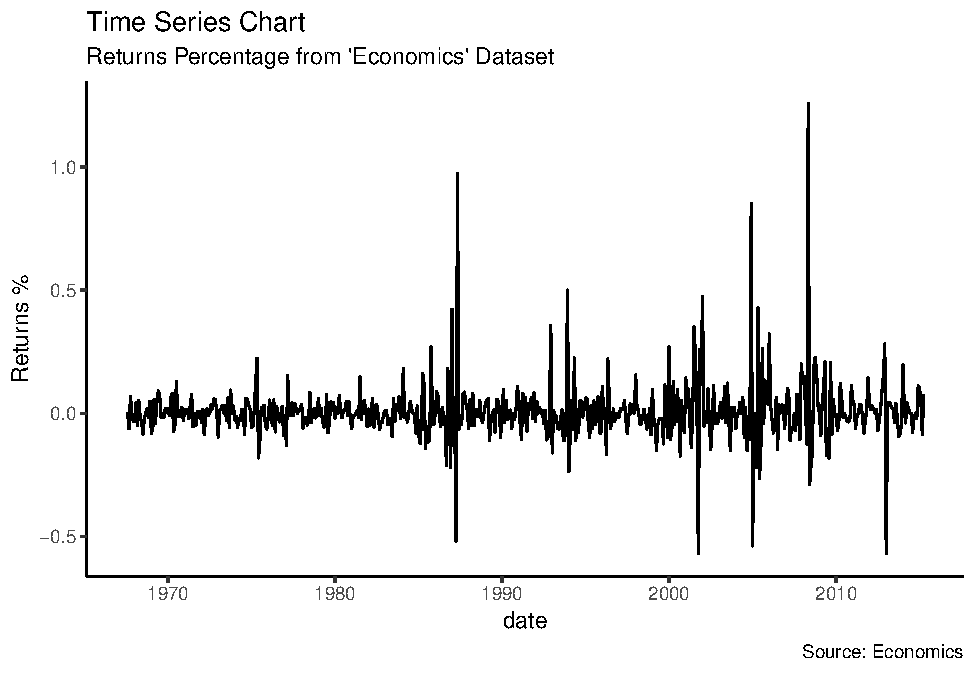
\includegraphics{ggplot2-50examples_files/figure-latex/unnamed-chunk-42-1.pdf}

\newpage

\textbf{Calendar Heatmap}

When you want to see the variation, especially the highs and lows, of a
metric like stock price, on an actual calendar itself, the calendar heat
map is a great tool. It emphasizes the variation visually over time
rather than the actual value itself.

This can be implemented using the geom\_tile. But getting it in the
right format has more to do with the data preparation rather than the
plotting itself.

\begin{Shaded}
\begin{Highlighting}[]
\CommentTok{# http://margintale.blogspot.in/2012/04/ggplot2-time-series-heatmaps.html}
\KeywordTok{library}\NormalTok{(ggplot2)}
\KeywordTok{library}\NormalTok{(plyr)}
\end{Highlighting}
\end{Shaded}

\begin{verbatim}
## 
## Attaching package: 'plyr'
\end{verbatim}

\begin{verbatim}
## The following object is masked from 'package:lubridate':
## 
##     here
\end{verbatim}

\begin{Shaded}
\begin{Highlighting}[]
\KeywordTok{library}\NormalTok{(scales)}
\KeywordTok{library}\NormalTok{(zoo)}

\NormalTok{df <-}\StringTok{ }\KeywordTok{read.csv}\NormalTok{(}\StringTok{"https://raw.githubusercontent.com/selva86/datasets/master/yahoo.csv"}\NormalTok{)}
\NormalTok{df}\OperatorTok{$}\NormalTok{date <-}\StringTok{ }\KeywordTok{as.Date}\NormalTok{(df}\OperatorTok{$}\NormalTok{date)  }\CommentTok{# format date}
\NormalTok{df <-}\StringTok{ }\NormalTok{df[df}\OperatorTok{$}\NormalTok{year }\OperatorTok{>=}\StringTok{ }\DecValTok{2012}\NormalTok{, ]  }\CommentTok{# filter reqd years}

\CommentTok{# Create Month Week}
\NormalTok{df}\OperatorTok{$}\NormalTok{yearmonth <-}\StringTok{ }\KeywordTok{as.yearmon}\NormalTok{(df}\OperatorTok{$}\NormalTok{date)}
\NormalTok{df}\OperatorTok{$}\NormalTok{yearmonthf <-}\StringTok{ }\KeywordTok{factor}\NormalTok{(df}\OperatorTok{$}\NormalTok{yearmonth)}
\NormalTok{df <-}\StringTok{ }\KeywordTok{ddply}\NormalTok{(df,.(yearmonthf), transform, }\DataTypeTok{monthweek=}\DecValTok{1}\OperatorTok{+}\NormalTok{week}\OperatorTok{-}\KeywordTok{min}\NormalTok{(week))  }
\CommentTok{# compute week number of month}
\NormalTok{df <-}\StringTok{ }\NormalTok{df[, }\KeywordTok{c}\NormalTok{(}\StringTok{"year"}\NormalTok{, }\StringTok{"yearmonthf"}\NormalTok{, }\StringTok{"monthf"}\NormalTok{, }\StringTok{"week"}\NormalTok{, }\StringTok{"monthweek"}\NormalTok{, }\StringTok{"weekdayf"}\NormalTok{, }\StringTok{"VIX.Close"}\NormalTok{)]}
\KeywordTok{head}\NormalTok{(df)}
\end{Highlighting}
\end{Shaded}

\begin{verbatim}
##   year yearmonthf monthf week monthweek weekdayf VIX.Close
## 1 2012     1 2012    Jan    1         1      Tue     22.97
## 2 2012     1 2012    Jan    1         1      Wed     22.22
## 3 2012     1 2012    Jan    1         1      Thu     21.48
## 4 2012     1 2012    Jan    1         1      Fri     20.63
## 5 2012     1 2012    Jan    2         2      Mon     21.07
## 6 2012     1 2012    Jan    2         2      Tue     20.69
\end{verbatim}

\begin{Shaded}
\begin{Highlighting}[]
\CommentTok{# Plot}
\KeywordTok{ggplot}\NormalTok{(df, }\KeywordTok{aes}\NormalTok{(monthweek, weekdayf, }\DataTypeTok{fill =}\NormalTok{ VIX.Close)) }\OperatorTok{+}\StringTok{ }
\StringTok{  }\KeywordTok{geom_tile}\NormalTok{(}\DataTypeTok{colour =} \StringTok{"white"}\NormalTok{) }\OperatorTok{+}\StringTok{ }
\StringTok{  }\KeywordTok{facet_grid}\NormalTok{(year}\OperatorTok{~}\NormalTok{monthf) }\OperatorTok{+}\StringTok{ }
\StringTok{  }\KeywordTok{scale_fill_gradient}\NormalTok{(}\DataTypeTok{low=}\StringTok{"red"}\NormalTok{, }\DataTypeTok{high=}\StringTok{"green"}\NormalTok{) }\OperatorTok{+}
\StringTok{  }\KeywordTok{labs}\NormalTok{(}\DataTypeTok{x=}\StringTok{"Week of Month"}\NormalTok{,}
       \DataTypeTok{y=}\StringTok{""}\NormalTok{,}
       \DataTypeTok{title =} \StringTok{"Time-Series Calendar Heatmap"}\NormalTok{, }
       \DataTypeTok{subtitle=}\StringTok{"Yahoo Closing Price"}\NormalTok{, }
       \DataTypeTok{fill=}\StringTok{"Close"}\NormalTok{)}
\end{Highlighting}
\end{Shaded}

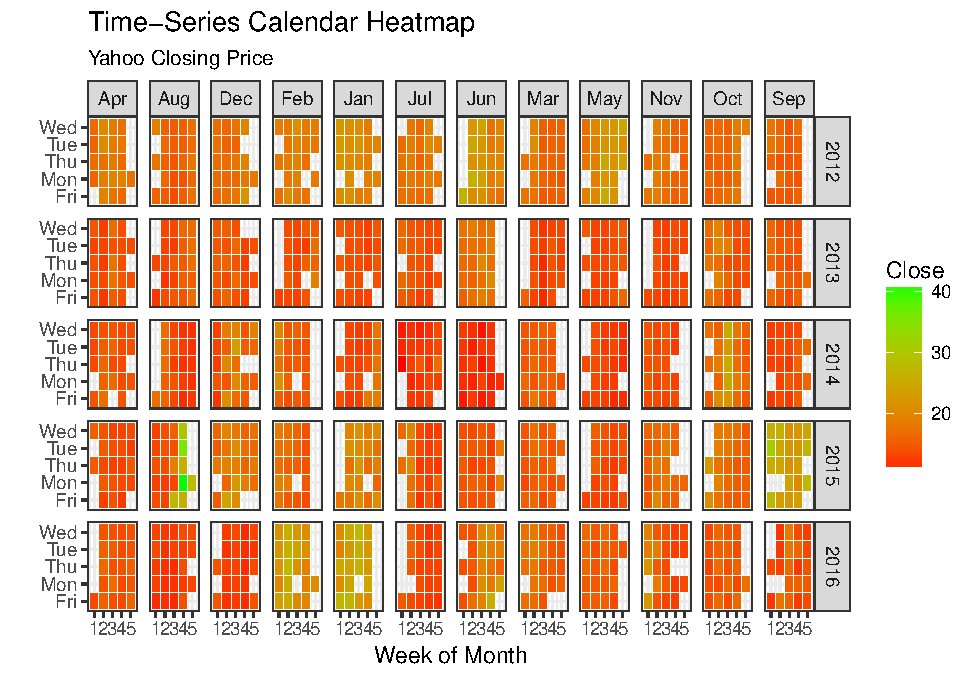
\includegraphics{ggplot2-50examples_files/figure-latex/unnamed-chunk-43-1.pdf}

\newpage

\newpage

\textbf{Seasonal Plot}

If you are working with a time series object of class ts or xts, you can
view the seasonal fluctuations through a seasonal plot drawn using
\texttt{forecast::ggseasonplot}. Below is an example using the native
AirPassengers and nottem time series.

You can see the traffic increase in air passengers over the years along
with the repetitive seasonal patterns in traffic. Whereas Nottingham
does not show an increase in overal temperatures over the years, but
they definitely follow a seasonal pattern.

\begin{Shaded}
\begin{Highlighting}[]
\KeywordTok{library}\NormalTok{(ggplot2)}
\KeywordTok{library}\NormalTok{(forecast)}
\KeywordTok{theme_set}\NormalTok{(}\KeywordTok{theme_classic}\NormalTok{())}

\CommentTok{# Subset data}
\NormalTok{nottem_small <-}\StringTok{ }\KeywordTok{window}\NormalTok{(nottem, }\DataTypeTok{start=}\KeywordTok{c}\NormalTok{(}\DecValTok{1920}\NormalTok{, }\DecValTok{1}\NormalTok{), }\DataTypeTok{end=}\KeywordTok{c}\NormalTok{(}\DecValTok{1925}\NormalTok{, }\DecValTok{12}\NormalTok{))  }
\CommentTok{# subset a smaller timewindow}

\CommentTok{# Plot}
\KeywordTok{ggseasonplot}\NormalTok{(AirPassengers) }\OperatorTok{+}\StringTok{ }\KeywordTok{labs}\NormalTok{(}\DataTypeTok{title=}\StringTok{"Seasonal plot: International Airline Passengers"}\NormalTok{)}
\end{Highlighting}
\end{Shaded}

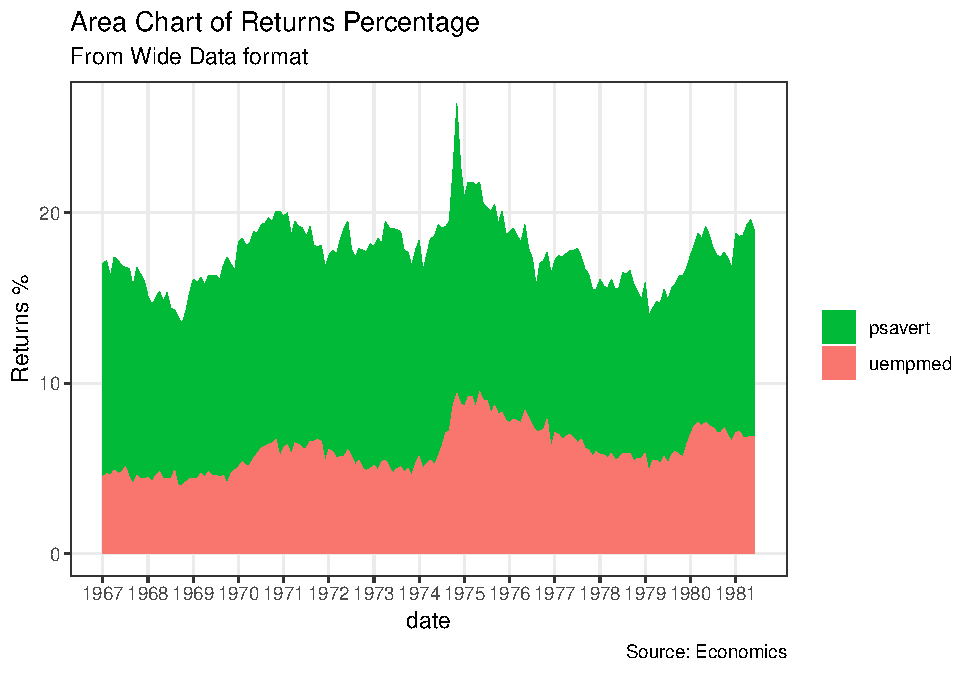
\includegraphics{ggplot2-50examples_files/figure-latex/unnamed-chunk-47-1.pdf}

\begin{Shaded}
\begin{Highlighting}[]
\KeywordTok{ggseasonplot}\NormalTok{(nottem_small) }\OperatorTok{+}\StringTok{ }\KeywordTok{labs}\NormalTok{(}\DataTypeTok{title=}\StringTok{"Seasonal plot: Air temperatures at Nottingham Castle"}\NormalTok{)}
\end{Highlighting}
\end{Shaded}

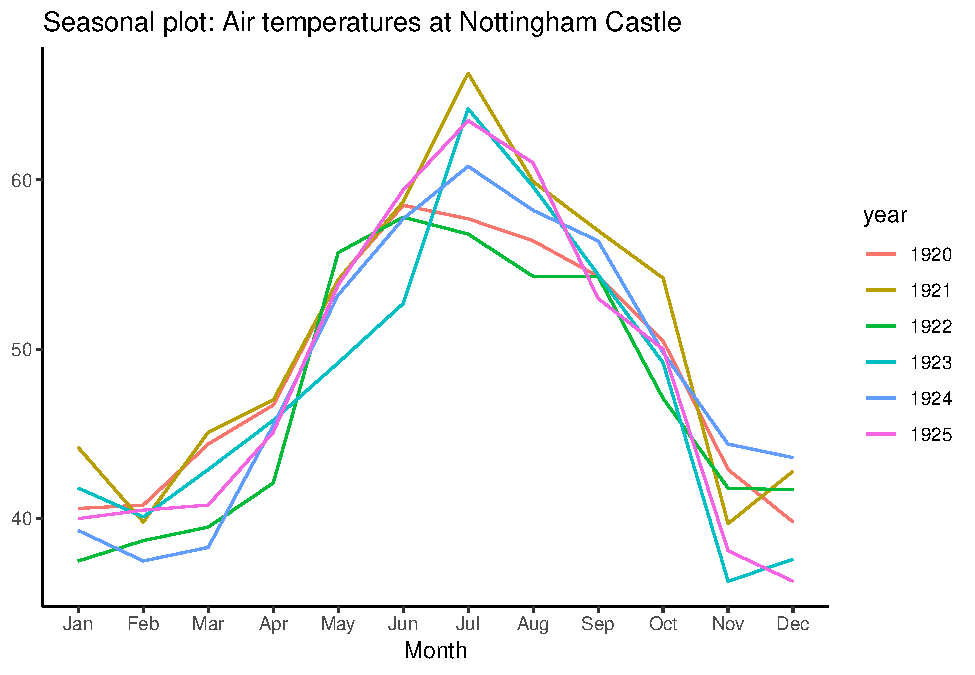
\includegraphics{ggplot2-50examples_files/figure-latex/unnamed-chunk-47-2.pdf}

\newpage

\subsection{7. Groups}\label{groups}

\textbf{Hierarchical Dendrogram}

\begin{Shaded}
\begin{Highlighting}[]
\CommentTok{# install.packages("ggdendro")}
\KeywordTok{library}\NormalTok{(ggplot2)}
\KeywordTok{library}\NormalTok{(ggdendro)}
\KeywordTok{theme_set}\NormalTok{(}\KeywordTok{theme_bw}\NormalTok{())}

\NormalTok{hc <-}\StringTok{ }\KeywordTok{hclust}\NormalTok{(}\KeywordTok{dist}\NormalTok{(USArrests), }\StringTok{"ave"}\NormalTok{)  }\CommentTok{# hierarchical clustering}

\CommentTok{# plot}
\KeywordTok{ggdendrogram}\NormalTok{(hc, }\DataTypeTok{rotate =} \OtherTok{TRUE}\NormalTok{, }\DataTypeTok{size =} \DecValTok{2}\NormalTok{)}
\end{Highlighting}
\end{Shaded}

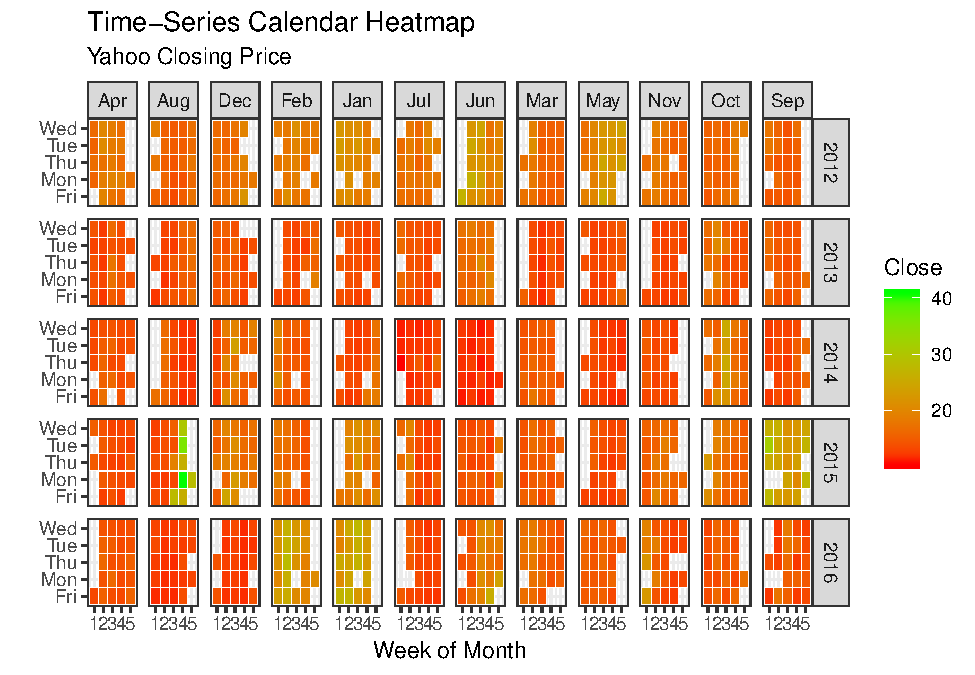
\includegraphics{ggplot2-50examples_files/figure-latex/unnamed-chunk-48-1.pdf}

\newpage

blank

\newpage

\textbf{Clusters}

It is possible to show the distinct clusters or groups using
\texttt{geom\_encircle()}. If the dataset has multiple weak features,
you can compute the principal components and draw a scatterplot using
PC1 and PC2 as X and Y axis.

The \texttt{geom\_encircle()} can be used to encircle the desired
groups. The only thing to note is the data argument to geom\_circle().
You need to provide a subsetted dataframe that contains only the
observations (rows) that belong to the group as the data argument.

\begin{Shaded}
\begin{Highlighting}[]
\CommentTok{# devtools::install_github("hrbrmstr/ggalt")}
\KeywordTok{library}\NormalTok{(ggplot2)}
\KeywordTok{library}\NormalTok{(ggalt)}
\KeywordTok{library}\NormalTok{(ggfortify)}
\KeywordTok{theme_set}\NormalTok{(}\KeywordTok{theme_classic}\NormalTok{())}

\CommentTok{# Compute data with principal components ------------------}
\NormalTok{df <-}\StringTok{ }\NormalTok{iris[}\KeywordTok{c}\NormalTok{(}\DecValTok{1}\NormalTok{, }\DecValTok{2}\NormalTok{, }\DecValTok{3}\NormalTok{, }\DecValTok{4}\NormalTok{)]}
\NormalTok{pca_mod <-}\StringTok{ }\KeywordTok{prcomp}\NormalTok{(df)  }\CommentTok{# compute principal components}

\CommentTok{# Data frame of principal components ----------------------}
\NormalTok{df_pc <-}\StringTok{ }\KeywordTok{data.frame}\NormalTok{(pca_mod}\OperatorTok{$}\NormalTok{x, }\DataTypeTok{Species=}\NormalTok{iris}\OperatorTok{$}\NormalTok{Species)  }\CommentTok{# dataframe of principal components}
\NormalTok{df_pc_vir <-}\StringTok{ }\NormalTok{df_pc[df_pc}\OperatorTok{$}\NormalTok{Species }\OperatorTok{==}\StringTok{ "virginica"}\NormalTok{, ]  }\CommentTok{# df for 'virginica'}
\NormalTok{df_pc_set <-}\StringTok{ }\NormalTok{df_pc[df_pc}\OperatorTok{$}\NormalTok{Species }\OperatorTok{==}\StringTok{ "setosa"}\NormalTok{, ]  }\CommentTok{# df for 'setosa'}
\NormalTok{df_pc_ver <-}\StringTok{ }\NormalTok{df_pc[df_pc}\OperatorTok{$}\NormalTok{Species }\OperatorTok{==}\StringTok{ "versicolor"}\NormalTok{, ]  }\CommentTok{# df for 'versicolor'}
 
\CommentTok{# Plot ----------------------------------------------------}
\KeywordTok{ggplot}\NormalTok{(df_pc, }\KeywordTok{aes}\NormalTok{(PC1, PC2, }\DataTypeTok{col=}\NormalTok{Species)) }\OperatorTok{+}\StringTok{ }
\StringTok{  }\KeywordTok{geom_point}\NormalTok{(}\KeywordTok{aes}\NormalTok{(}\DataTypeTok{shape=}\NormalTok{Species), }\DataTypeTok{size=}\DecValTok{2}\NormalTok{) }\OperatorTok{+}\StringTok{   }\CommentTok{# draw points}
\StringTok{  }\KeywordTok{labs}\NormalTok{(}\DataTypeTok{title=}\StringTok{"Iris Clustering"}\NormalTok{, }
       \DataTypeTok{subtitle=}\StringTok{"With principal components PC1 and PC2 as X and Y axis"}\NormalTok{,}
       \DataTypeTok{caption=}\StringTok{"Source: Iris"}\NormalTok{) }\OperatorTok{+}\StringTok{ }
\StringTok{  }\KeywordTok{coord_cartesian}\NormalTok{(}\DataTypeTok{xlim =} \FloatTok{1.2} \OperatorTok{*}\StringTok{ }\KeywordTok{c}\NormalTok{(}\KeywordTok{min}\NormalTok{(df_pc}\OperatorTok{$}\NormalTok{PC1), }\KeywordTok{max}\NormalTok{(df_pc}\OperatorTok{$}\NormalTok{PC1)), }
                  \DataTypeTok{ylim =} \FloatTok{1.2} \OperatorTok{*}\StringTok{ }\KeywordTok{c}\NormalTok{(}\KeywordTok{min}\NormalTok{(df_pc}\OperatorTok{$}\NormalTok{PC2), }\KeywordTok{max}\NormalTok{(df_pc}\OperatorTok{$}\NormalTok{PC2))) }\OperatorTok{+}\StringTok{   }\CommentTok{# change axis limits}
\StringTok{  }\KeywordTok{geom_encircle}\NormalTok{(}\DataTypeTok{data =}\NormalTok{ df_pc_vir, }\KeywordTok{aes}\NormalTok{(}\DataTypeTok{x=}\NormalTok{PC1, }\DataTypeTok{y=}\NormalTok{PC2)) }\OperatorTok{+}\StringTok{   }\CommentTok{# draw circles}
\StringTok{  }\KeywordTok{geom_encircle}\NormalTok{(}\DataTypeTok{data =}\NormalTok{ df_pc_set, }\KeywordTok{aes}\NormalTok{(}\DataTypeTok{x=}\NormalTok{PC1, }\DataTypeTok{y=}\NormalTok{PC2)) }\OperatorTok{+}\StringTok{ }
\StringTok{  }\KeywordTok{geom_encircle}\NormalTok{(}\DataTypeTok{data =}\NormalTok{ df_pc_ver, }\KeywordTok{aes}\NormalTok{(}\DataTypeTok{x=}\NormalTok{PC1, }\DataTypeTok{y=}\NormalTok{PC2))}
\end{Highlighting}
\end{Shaded}

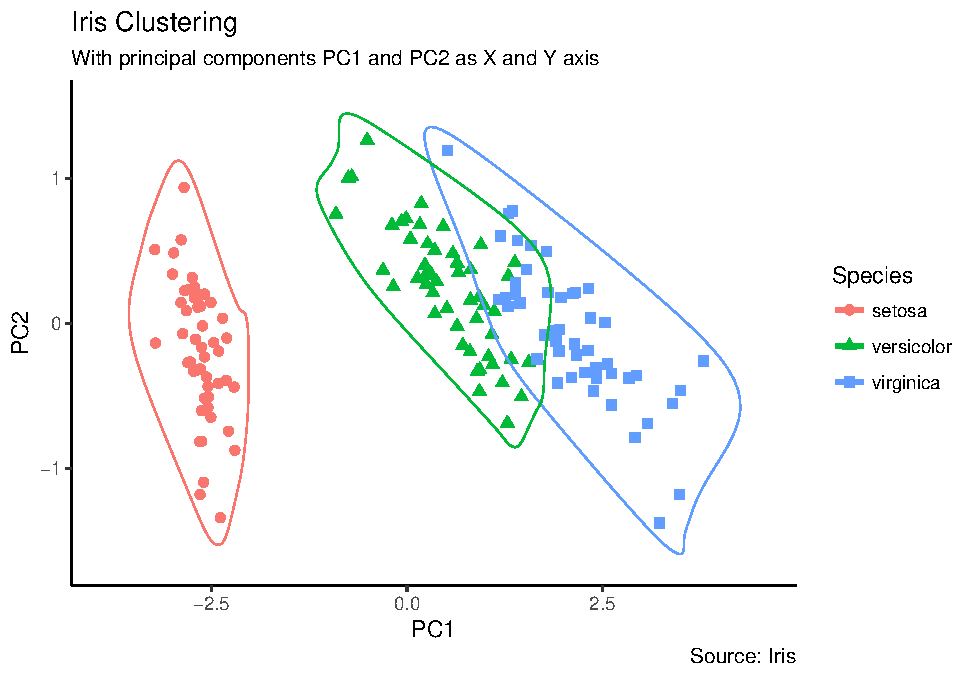
\includegraphics{ggplot2-50examples_files/figure-latex/unnamed-chunk-49-1.pdf}

REFERENCE:
\url{http://r-statistics.co/Top50-Ggplot2-Visualizations-MasterList-R-Code.html}


\end{document}
